% ====================================================================
%  徐森林、薛春华《数学分析》（第一册）
%  第 2 章  函数极限与连续
%  源：原书印刷页 81-152（PDF 物理页 = 印刷页 + 6）
% ====================================================================

\chapter{函数极限与连续}\label{ch:2}

数列是一种特殊的函数, 上一章已经详细地讨论了这个特殊函数的极限, 并学会了很多求极限的方法, 这给本章要讨论的一般函数的极限打下了良好的基础, 有时数列极限可化为求函数极限. 本章将介绍函数的极限与函数的连续以及它们的一些性质, 并给出闭区间上连续函数若干重要定理: 零值定理、介值定理、最值定理、一致连续性定理, 这些定理在数学分析与实际问题中都有广泛的应用.

% ====================================================================
%  徐森林、薛春华《数学分析》（第一册）
%  \S2.1  函数极限的概念
%  源：原书印刷页 81-99（PDF 物理页 87-105）
% ====================================================================
\section{函数极限的概念}\label{sec:2.1}

温故而知新, 先复习一下映射和函数的概念.

\begin{definition}\label{def:2.1.1}
设 $X, Y$ 为非空集合, 如果对 $\forall x \in X$, 有惟一的 $y \in Y$ 与之对应, 表示为 $y = f(x)$, 其中 $x$ 称为自变量或原像点, $y$ 称为因变量或像点, $f$ 称为(单值)映射或对应规律, 记作
\[
f\colon X\to Y,\quad x\mapsto y = f(x).
\]
$X$ 称为 $f$ 的\textbf{定义域},
\[
f(X)=\{f(x)\mid x\in X\}
\]
称为 $f$ 的\textbf{值域},
\[
f(A)=\{f(x)\mid x\in A\subset X\}\subset Y
\]
称为 $A$ 在 $f$ 下的\textbf{像}.
\[
f^{-1}(B)=\{x\in X\mid f(x)\in B\}\subset X
\]
为 $B$ 在 $f$ 下的\textbf{原像}.
\end{definition}

$f$ 的表示法有下面几种.

(1) \textbf{解析式法}: 如 $y=x^{2}$, $y=e^{x}$, $y=\sin x$.

(2) \textbf{列表法}: $y=f(x)=x^{2}$ 图表为
\begin{center}
\begin{tabular}{c|ccccc}
\hline
$x$ & $1$ & $2$ & $3$ & $\cdots$ \\
\hline
$y$ & $1$ & $4$ & $9$ & $\cdots$ \\
\hline
\end{tabular}
\end{center}

(3) \textbf{图像法}: $y = f(x) = x^{2}$ 的图像为抛物线. 画图先列表、描点再连成曲线(如图~\ref{fig:2.1.1} 所示).

\begin{figure}[htbp]
\centering
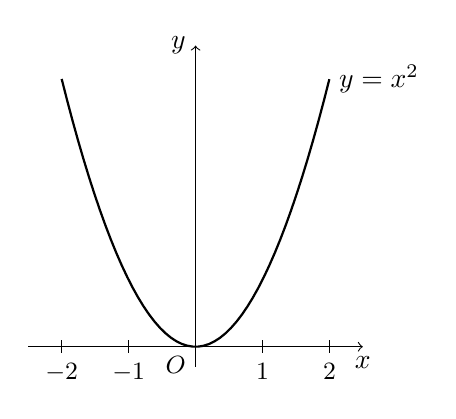
\begin{tikzpicture}[scale=0.85]
  \draw[->] (-2.5,0) -- (2.5,0) node[below] {$x$};
  \draw[->] (0,-0.3) -- (0,4.5) node[left] {$y$};
  \draw[thick, domain=-2:2, samples=50] plot (\x, {\x*\x});
  \node[right] at (2,4) {$y=x^2$};
  \foreach \x in {-2,-1,1,2} {
    \draw (\x,0.1) -- (\x,-0.1) node[below] {\small $\x$};
  }
  \node[below left] at (0,0) {\small $O$};
\end{tikzpicture}
\caption{}\label{fig:2.1.1}
\end{figure}

如果 $\forall x_{1}, x_{2} \in X, x_{1} \neq x_{2}$, 必有 $f(x_{1}) \neq f(x_{2})$, 即若 $f(x_{1})=f(x_{2})$, 必有 $x_{1}=x_{2}$, 则称 $f$ 为\textbf{单射}; 如果 $\forall y\in Y$, 必 $\exists x\in X$, s.t. $f(x)=y$, 则称 $f$ 为\textbf{满射}.

如果 $f$ 既为单射又为满射, 则称 $f$ 为\textbf{双射}或\textbf{一一映射}. 此时, $f$ 有逆映射 $f^{-1}\colon Y \to X$, $x = f^{-1}(y)$ (即 $y = f(x)$). 显然, 当 $f$ 为单射时, $f\colon X \to f(X)$ 就为双射或一一映射.

设 $X$ 为非空集合, $f\colon X \to \mathbb{R}$, $x \mapsto y = f(x)$ 为映射, 则称 $f$ 为\textbf{实(值)函数}, 本书中简称为\textbf{函数}.
\begin{itemize}
  \item 若 $X \subset \mathbb{R}$, 则称 $f$ 为一元(单变量)函数;
  \item 若 $X \subset \mathbb{R}^{2} = \{(x, y) \mid x, y \in \mathbb{R}\}$, 则称 $f$ 为二元函数;
  \item 若 $X \subset \mathbb{R}^{3} = \{(x, y, z) \mid x, y, z \in \mathbb{R}\}$, 则称 $f$ 为三元函数;
  \item 若 $X \subset \mathbb{R}^{n} = \{(x_{1}, x_{2}, \cdots, x_{n}) \mid x_{i} \in \mathbb{R}, i=1,2,\cdots,n\}$, 则称 $f$ 为 $n$ 元函数.
\end{itemize}

设 $f, g\colon X \to \mathbb{R}$, $x \in X$, 令
\begin{align*}
(f\pm g)(x) &= f(x)\pm g(x), \\
(fg)(x) &= f(x)g(x), \\
\frac{f}{g}(x) &= \frac{f(x)}{g(x)}\quad (g(x)\neq 0).
\end{align*}
它们分别定义了 $f$ 与 $g$ 的和函数 $f + g$, 差函数 $f - g$, 积函数 $fg$ 及商函数 $\frac{f}{g}$.

设 $f\colon X \to Y$, $g\colon Y \to Z$, 则称 $g \circ f\colon X \to Z$, $x \mapsto z = g \circ f(x) = g(f(x))$ 为 $f$ 与 $g$ 的复合. 两个函数 $f, g$ 的复合称为 $f$ 与 $g$ 的复合函数(如图~\ref{fig:2.1.2} 所示). 关于复合显然有 $(g \circ f) \circ h = g \circ (f \circ h)$.

\begin{figure}[htbp]
\centering
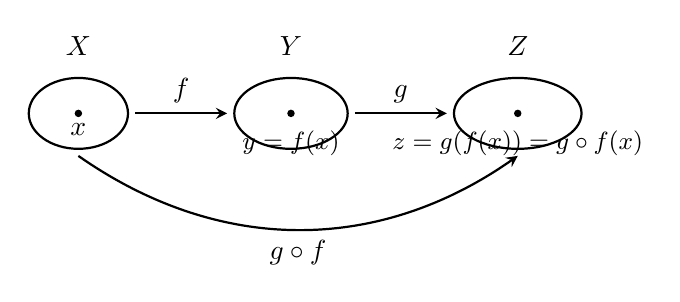
\begin{tikzpicture}[scale=0.9, >=stealth]
  \draw[thick] (0,0) ellipse (0.7cm and 0.5cm) node[above=0.6cm] {$X$};
  \fill (0,0) circle (1.5pt) node[below] {$x$};
  
  \draw[thick] (3.0,0) ellipse (0.8cm and 0.5cm) node[above=0.6cm] {$Y$};
  \fill (3.0,0) circle (1.5pt) node[below=0.1cm] {\small $y=f(x)$};
  
  \draw[thick] (6.2,0) ellipse (0.9cm and 0.5cm) node[above=0.6cm] {$Z$};
  \fill (6.2,0) circle (1.5pt) node[below=0.1cm] {\small $z=g(f(x))=g\circ f(x)$};
  
  \draw[->, thick] (0.8,0) -- (2.1,0) node[midway, above] {$f$};
  \draw[->, thick] (3.9,0) -- (5.2,0) node[midway, above] {$g$};
  \draw[->, thick] (0,-0.6) to[out=-35,in=-145] node[midway, below] {$g\circ f$} (6.2,-0.6);
\end{tikzpicture}
\caption{}\label{fig:2.1.2}
\end{figure}

中学里已学的基本初等函数共有 6 类:

(1) \textbf{常值函数} $y=f(x)=c$, 定义域为 $\mathbb{R}$.

(2) \textbf{幂函数} $y = f(x) = x^{\alpha}$ ($\alpha$ 为实数). 当 $x > 0$ 时, 任何 $\alpha$ 都有意义; $x^{n}\ (n \in \mathbb{N})$ 的定义域为实数集 $\mathbb{R}$; $x^{-n}\ (n \in \mathbb{N})$ 的定义域为 $\mathbb{R} \setminus \{0\}$; $x^{\frac{1}{2}} = \sqrt{x}$ 的定义域为 $[0, +\infty)$; $x^{-\frac{1}{2}}$ 的定义域为 $(0, +\infty)$; $x^{\frac{1}{3}}$ 的定义域为 $\mathbb{R}$; $x^{-\frac{1}{3}}$ 的定义域为 $\mathbb{R} \setminus \{0\}$; 等等.

(3) \textbf{三角函数} $y=\sin x, \cos x$ 定义域都为 $\mathbb{R}$; $y=\tan x$, 定义域为 $\mathbb{R} \setminus \{k\pi + \frac{\pi}{2}, k \in \mathbb{Z}\}$; $y=\cot x$, 定义域为 $\mathbb{R} \setminus \{k\pi, k \in \mathbb{Z}\}$; $y=\sec x$, 定义域为 $\mathbb{R} \setminus \{k\pi + \frac{\pi}{2}, k \in \mathbb{Z}\}$; $y=\csc x$, 定义域为 $\mathbb{R} \setminus \{k\pi, k \in \mathbb{Z}\}$.

(4) \textbf{反三角函数} $y=\arcsin x, \arccos x$ 定义域为 $[-1,1]$; $y=\arctan x, \operatorname{arccot} x$ 定义域为 $\mathbb{R}$.

(5) \textbf{指数函数} $y=a^{x}\ (a>0,a\neq1)$, 定义域为 $\mathbb{R}$.

(6) \textbf{对数函数} $y=\log_{a}x\ (a>0,a\neq1)$, 定义域为 $(0,+\infty)$. 特别地, 常用对数记作 $\lg x = \log_{10}x$, 自然对数记作 $\ln x = \log_{\mathrm{e}}x$.

读者应记住每个基本初等函数的值域, 并画出相应的图形.

\begin{definition}\label{def:2.1.2}
由基本初等函数通过有限次 $+$, $-$, $\cdot$, $\div$ 和复合得到的函数称为\textbf{初等函数}. 这是一类重要的函数.
\end{definition}

再给出几类今后要常用的函数.

\begin{example}\label{ex:2.1.1}
证明:
\begin{enumerate}[label=(\arabic*)]
  \item 双曲函数:
  \begin{align*}
  \sinh x &= \frac{e^{x}-e^{-x}}{2},\quad \cosh x=\frac{e^{x}+e^{-x}}{2}, \\
  \tanh x &= \frac{\sinh x}{\cosh x}=\frac{e^{x}-e^{-x}}{e^{x}+e^{-x}},\quad \coth x=\frac{\cosh x}{\sinh x}=\frac{e^{x}+e^{-x}}{e^{x}-e^{-x}}
\end{align*}
  都是初等函数. 读者经过验算可知双曲函数具有性质:
  \[
  \sinh 2x=2\sinh x\cosh x,\quad \cosh 2x=\cosh^{2}x+\sinh^{2}x,\quad \cosh^{2}x-\sinh^{2}x=1.
\]
  \item $y=\ln(x+\sqrt{x^{2}+1})$ 为初等函数.
  \item $y=|x|=\begin{cases} x, & x\geqslant0, \\ -x, & x<0 \end{cases}$ 为初等函数.
  \item 多项式函数 $y = a_{0}x^{n} + a_{1}x^{n-1} + \cdots + a_{n-1}x + a_{n}\ (a_{0} \neq 0)$ 与有理函数
  \[
  y = \frac{a_{0}x^{n} + a_{1}x^{n-1} + \cdots + a_{n-1}x + a_{n}}{b_{0}x^{m} + b_{1}x^{m-1} + \cdots + b_{m-1}x + b_{m}}\quad (a_{0} \neq 0, b_{0} \neq 0)
\]
  均为初等函数.
\end{enumerate}
\end{example}

\begin{proof}
(1) 以 $y = \tanh x$ 为例证明双曲函数为初等函数. 因为 $y = \tanh x = \frac{e^{x} - e^{-x}}{e^{x} + e^{-x}}$ 为基本初等函数 $e^{x}, e^{-x} = (e^{-1})^{x}$ 通过一次减法、一次加法、一次除法得到, 所以它为初等函数. 或者因为 $y = \tanh x = \frac{e^{x} - \frac{1}{e^{x}}}{e^{x} + \frac{1}{e^{x}}}$ 为基本初等函数 $e^{x}, 1$ 通过一次减法, 一次加法, 三次除法得到, 所以它为初等函数. 其他类似证明.

(2) 因为 $y=\ln(x+\sqrt{x^{2}+1})$ 由基本初等函数 $x, x^{2}, 1, \sqrt{x}, \ln x$ 通过两次加法, 两次复合得到, 所以它为初等函数.

(3) 因为 $y=|x|=\sqrt{x^{2}}$ 为基本初等函数 $x^{2}, \sqrt{x}$ 通过一次复合得到, 所以它为初等函数.

(4) 因为多项式函数 $y=a_{0}x^{n}+\cdots+a_{n}$ 为基本初等函数 $a_{0}, \cdots, a_{n}, x, \cdots, x^{n}$ 通过 $n$ 次乘法与 $n$ 次加法得到, 所以它为初等函数.

而有理函数为基本初等函数通过有限次乘法、加法以及除法得到, 所以它为初等函数.
\end{proof}

\begin{example}\label{ex:2.1.2}
\begin{enumerate}[label=(\arabic*)]
  \item 设 $f_{1}, f_{2}, \cdots, f_{n}$ 都为初等函数, 则由 $f_{1}, f_{2}, \cdots, f_{n}$ 经有限次 $+$, $-$, $\cdot$, $\div$, 复合运算得到的函数 $f$ 仍为初等函数.
  \item 设 $f, g$ 都为初等函数, 则 $\max\{f, g\}$ 与 $\min\{f, g\}$ 均为初等函数.
\end{enumerate}
\end{example}

\begin{proof}
(1) 因为 $f_{1}, f_{2}, \cdots, f_{n}$ 都为初等函数, 所以它们都由基本初等函数通过有限次 $+$, $-$, $\cdot$, $\div$, 复合运算得到. 从而, 由 $f_{1}, f_{2}, \cdots, f_{n}$ 经有限次 $+$, $-$, $\cdot$, $\div$, 复合运算得到的函数 $f$ 也由基本初等函数通过有限次 $+$, $-$, $\cdot$, $\div$, 复合运算得到, 该函数 $f$ 应是初等函数.

(2) 由 $f, g$ 都为初等函数及
\begin{align*}
\max\{f,g\} &= \frac{(f+g)+|f-g|}{2}=\frac{(f+g)+\sqrt{(f-g)^2}}{2}, \\
\min\{f,g\} &= \frac{(f+g)-|f-g|}{2}=\frac{(f+g)-\sqrt{(f-g)^2}}{2}
\end{align*}
或 $\min\{f,g\} = -\max\{-f,-g\}$ 可知 $\max\{f,g\}$ 与 $\min\{f,g\}$ 均为初等函数.
\end{proof}

另一类重要的函数就是\textbf{分段函数}, 即每一段上用不同的式子表达的函数.

\begin{example}\label{ex:2.1.3}
\begin{enumerate}[label=(\arabic*)]
  \item \textbf{符号函数}(如图~\ref{fig:2.1.3} 所示):
  \[
  y=\operatorname{sgn} x=\begin{cases}
  1, & x>0, \\
  0, & x=0, \\
  -1, & x<0.
\end{cases}
\]
  \item \textbf{“取整数”函数}(如图~\ref{fig:2.1.4} 所示):
  \[
  y=\lfloor x\rfloor = [x]
\]
  为不大于 $x$ 的最大整数, 此时有 $x-1<[x]\leqslant x<[x]+1$.
\end{enumerate}
\end{example}

\begin{figure}[htbp]
\centering
\begin{minipage}[t]{0.45\textwidth}
\centering
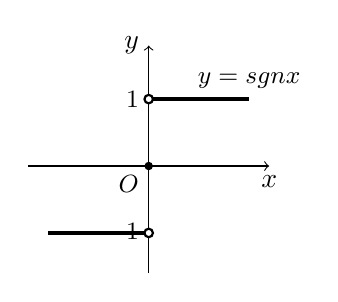
\begin{tikzpicture}[scale=0.85]
  \draw[->] (-1.8,0) -- (1.8,0) node[below] {$x$};
  \draw[->] (0,-1.6) -- (0,1.8) node[left] {$y$};
  \node[below left] at (0,0) {\small $O$};
  \draw[very thick] (0,1) -- (1.5,1) node[above, font=\small] {$y=\operatorname{sgn} x$};
  \draw[very thick] (-1.5,-1) -- (0,-1);
  \filldraw[fill=white, draw=black, thick] (0,1) circle (1.8pt);
  \filldraw[fill=white, draw=black, thick] (0,-1) circle (1.8pt);
  \fill (0,0) circle (1.8pt);
  \node[left] at (0,1) {\small $1$};
  \node[left] at (0,-1) {\small $-1$};
\end{tikzpicture}
\caption{}\label{fig:2.1.3}
\end{minipage}
\hfill
\begin{minipage}[t]{0.45\textwidth}
\centering
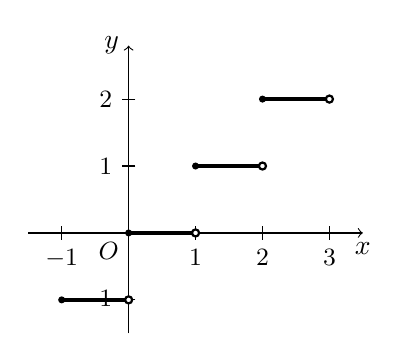
\begin{tikzpicture}[scale=0.85]
  \draw[->] (-1.5,0) -- (3.5,0) node[below] {$x$};
  \draw[->] (0,-1.5) -- (0,2.8) node[left] {$y$};
  \node[below left] at (0,0) {\small $O$};
  \foreach \x in {-1,1,2,3} {
    \draw (\x,0.1) -- (\x,-0.1) node[below] {\small $\x$};
  }
  \foreach \y in {-1,1,2} {
    \draw (0.1,\y) -- (-0.1,\y) node[left] {\small $\y$};
  }
  \draw[very thick] (-1,-1) -- (0,-1);
  \fill (-1,-1) circle (1.5pt);
  \filldraw[fill=white, draw=black, thick] (0,-1) circle (1.5pt);
  
  \draw[very thick] (0,0) -- (1,0);
  \fill (0,0) circle (1.5pt);
  \filldraw[fill=white, draw=black, thick] (1,0) circle (1.5pt);
  
  \draw[very thick] (1,1) -- (2,1);
  \fill (1,1) circle (1.5pt);
  \filldraw[fill=white, draw=black, thick] (2,1) circle (1.5pt);
  
  \draw[very thick] (2,2) -- (3,2);
  \fill (2,2) circle (1.5pt);
  \filldraw[fill=white, draw=black, thick] (3,2) circle (1.5pt);
\end{tikzpicture}
\caption{}\label{fig:2.1.4}
\end{minipage}
\end{figure}

\begin{enumerate}[label=(\arabic*), resume]
  \item \textbf{尾数函数}(如图~\ref{fig:2.1.5} 所示):
  \[
  y=x-[x]\overset{\mathrm{def}}{=}\{x\},
\]
  则 $0\leqslant\{x\}<1$, 且 $\{x\}$ 是以 $1$ 为周期的函数.
  \item \textbf{绝对值函数}(如图~\ref{fig:2.1.6} 所示):
  \[
  y=|x|=\begin{cases}
  x, & x\geqslant0, \\
  -x, & x<0.
\end{cases}
\]
  \item 设 $A \subseteq \mathbb{R}$, $A$ 的\textbf{特征函数} $\chi_{A}\colon \mathbb{R} \to \mathbb{R}$,
  \[
  \chi_{A}(x)=\begin{cases}
  1, & x\in A, \\
  0, & x\in\mathbb{R}\setminus A\ (\text{即 } x\notin A).
\end{cases}
\]
  \item \textbf{Dirichlet 函数}:
  \[
  D(x)=\begin{cases}
  1, & x\in\mathbb{Q}, \\
  0, & x\in\mathbb{R}\setminus\mathbb{Q},
\end{cases}
\]
  它是 $\mathbb{Q}$ 的特征函数.
\end{enumerate}

以上 6 个函数都为分段函数.

\begin{figure}[htbp]
\centering
\begin{minipage}[t]{0.45\textwidth}
\centering
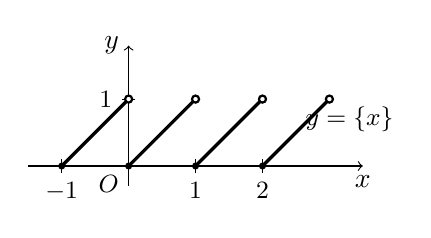
\begin{tikzpicture}[scale=0.85]
  \draw[->] (-1.5,0) -- (3.5,0) node[below] {$x$};
  \draw[->] (0,-0.3) -- (0,1.8) node[left] {$y$};
  \node[below left] at (0,0) {\small $O$};
  \draw (0.1,1) -- (-0.1,1) node[left] {\small $1$};
  \foreach \x in {-1,1,2} {
    \draw (\x,0.1) -- (\x,-0.1) node[below] {\small $\x$};
  }
  \foreach \k in {-1,0,1,2} {
    \draw[very thick] (\k,0) -- (\k+1,1);
    \fill (\k,0) circle (1.5pt);
    \filldraw[fill=white, draw=black, thick] (\k+1,1) circle (1.5pt);
  }
  \node[right, font=\small] at (2.5,0.7) {$y=\{x\}$};
\end{tikzpicture}
\caption{}\label{fig:2.1.5}
\end{minipage}
\hfill
\begin{minipage}[t]{0.45\textwidth}
\centering
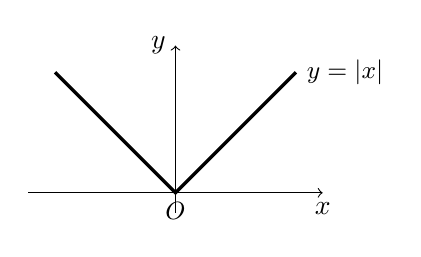
\begin{tikzpicture}[scale=0.85]
  \draw[->] (-2.2,0) -- (2.2,0) node[below] {$x$};
  \draw[->] (0,-0.3) -- (0,2.2) node[left] {$y$};
  \node[below] at (0,0) {\small $O$};
  \draw[very thick] (-1.8,1.8) -- (0,0) -- (1.8,1.8) node[right, font=\small] {$y=|x|$};
\end{tikzpicture}
\caption{}\label{fig:2.1.6}
\end{minipage}
\end{figure}

回想一下数列极限 $\lim\limits_{n\to+\infty}a_n=\lim\limits_{n\to+\infty}f(n)=a\in\mathbb{R}$ (收敛), $+\infty, -\infty, \infty$, 共有 4 种. 用 $N$ 刻画 $n$ 趋于 $+\infty$ 的程度, 用 $\varepsilon>0$ 刻画 $a_n$ 靠近 $a$ 的程度, 用 $A$ 刻画 $a_n$ 趋于 $+\infty, -\infty, \infty$ 的程度. 这里自变量只有一个趋向 $n\to+\infty$, 而一般函数 $f(x)$ 除了 $x\to+\infty$ 外, 还有 $x\to x_0, x_0^+, x_0^-, x\to-\infty, \infty$ 等情况.

我们考虑函数极限 $\lim\limits_{x \to x_{0}} f(x) = a \in \mathbb{R}$ (收敛), $+\infty, -\infty, \infty$ 时, 其中自变量趋向有 $x \to x_{0}, x \to x_{0}^{+}, x_{0}^{-}, +\infty, -\infty, \infty$ 共有 $6 \times 4 = 24$ 种不同情况, 我们用 $\delta > 0$ 刻画 $x$ 与 $x_{0}$ 或 $x$ 与 $x_{0}^{+}$ 或 $x$ 与 $x_{0}^{-}$ 的靠近程度, 用 $\Delta > 0$ 刻画 $x$ 趋于 $+\infty, -\infty, \infty$ 的程度, 用 $\varepsilon > 0$ 刻画 $f(x)$ 与 $a$ 靠近的程度, 用 $A$ 刻画 $f(x)$ 趋于 $+\infty, -\infty, \infty$ 的程度.

\begin{definition}\label{def:2.1.3}
设函数 $y = f(x)$ 在 $x_{0}$ 的一个去心开邻域 $(x_{0} - \delta_{0}, x_{0} + \delta_{0}) \setminus \{x_{0}\}$ 内有定义 ($x_{0}$ 处可以无定义). 如果有一数 $a \in \mathbb{R}$, s.t. $\forall \varepsilon > 0, \exists \delta \in (0, \delta_{0})$, 当 $0 < |x - x_{0}| < \delta$ 时, 有
\[
|f(x)-a|<\varepsilon,
\]
则称函数 $f(x)$ 在 $x_{0}$ 处(当 $x$ 趋于 $x_{0}$ 时)有极限 $a$, 记作 $\lim\limits_{x \to x_{0}} f(x) = a$, 或 $f(x) \to a\ (x \to x_{0})$ (如图~\ref{fig:2.1.7} 所示).

设函数 $y = f(x)$ 在 $x_{0}$ 去心右旁 $(x_{0}, x_{0} + \delta_{0})$ 有定义. 如果 $\forall A > 0, \exists \delta \in (0, \delta_{0})$, 当 $x_{0} < x < x_{0} + \delta$ 时, 有 $f(x) > A$, 则称函数 $f(x)$ 在 $x_{0}$ 的右旁(当 $x$ 趋于 $x_{0}^{+}$ 时)有右极限 $+\infty$, 记作 $f(x_{0} + 0) = f(x_{0}^{+}) = \lim\limits_{x \to x_{0}^{+}} f(x) = +\infty$, 或 $f(x) \to +\infty\ (x \to x_{0}^{+})$ (如图~\ref{fig:2.1.8} 所示).
\end{definition}

\begin{figure}[htbp]
\centering
\begin{minipage}[t]{0.45\textwidth}
\centering
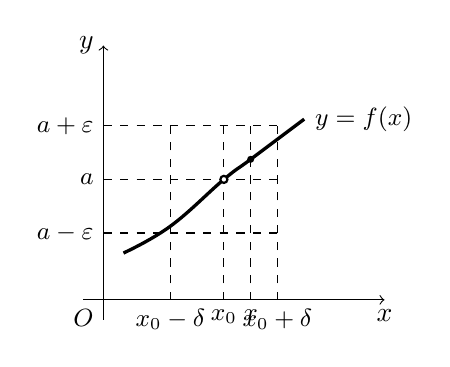
\begin{tikzpicture}[scale=0.85]
  \draw[->] (-0.3,0) -- (4.2,0) node[below] {$x$};
  \draw[->] (0,-0.3) -- (0,3.8) node[left] {$y$};
  \node[below left] at (0,0) {\small $O$};
  
  \draw[dashed] (1.0,0) node[below] {\small $x_0-\delta$} -- (1.0,2.6);
  \draw[dashed] (1.8,0) node[below] {\small $x_0$} -- (1.8,2.6);
  \draw[dashed] (2.2,0) node[below] {\small $x$} -- (2.2,2.6);
  \draw[dashed] (2.6,0) node[below] {\small $x_0+\delta$} -- (2.6,2.6);
  
  \draw[dashed] (0,1.0) node[left] {\small $a-\varepsilon$} -- (2.6,1.0);
  \draw[dashed] (0,1.8) node[left] {\small $a$} -- (2.6,1.8);
  \draw[dashed] (0,2.6) node[left] {\small $a+\varepsilon$} -- (2.6,2.6);
  
  \draw[very thick] plot [smooth, tension=0.7] coordinates {(0.3,0.7) (1.0,1.1) (1.8,1.8) (2.2,2.1) (3.0,2.7)} node[right, font=\small] {$y=f(x)$};
  \fill (2.2,2.1) circle (1.5pt);
  \filldraw[fill=white, draw=black, thick] (1.8,1.8) circle (1.5pt);
\end{tikzpicture}
\caption{}\label{fig:2.1.7}
\end{minipage}
\hfill
\begin{minipage}[t]{0.45\textwidth}
\centering
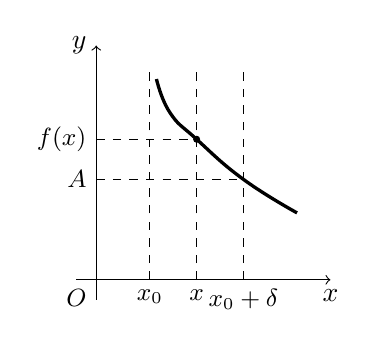
\begin{tikzpicture}[scale=0.85]
  \draw[->] (-0.3,0) -- (3.5,0) node[below] {$x$};
  \draw[->] (0,-0.3) -- (0,3.5) node[left] {$y$};
  \node[below left] at (0,0) {\small $O$};
  
  \draw[dashed] (0.8,0) node[below] {\small $x_0$} -- (0.8,3.2);
  \draw[dashed] (1.5,0) node[below] {\small $x$} -- (1.5,3.2);
  \draw[dashed] (2.2,0) node[below] {\small $x_0+\delta$} -- (2.2,3.2);
  
  \draw[dashed] (0,1.5) node[left] {\small $A$} -- (2.2,1.5);
  \draw[dashed] (0,2.1) node[left] {\small $f(x)$} -- (1.5,2.1);
  
  \draw[very thick] plot [smooth, tension=0.8] coordinates {(0.9,3.0) (1.1,2.5) (1.5,2.1) (2.2,1.5) (3.0,1.0)};
  \fill (1.5,2.1) circle (1.5pt);
\end{tikzpicture}
\caption{}\label{fig:2.1.8}
\end{minipage}
\end{figure}

设函数 $y = f(x)$ 在 $\infty$ 的开邻域 $(-\infty, -\Delta_{0}) \cup (\Delta_{0}, +\infty)$ 内有定义. 如果 $\forall A > 0, \exists \Delta > \Delta_{0} > 0$, 当 $|x| > \Delta$ 时, 有
\[
|f(x)|>A,
\]
则称函数 $y = f(x)$ 在 $\infty$ 处(当 $x \to \infty$ 时)有极限 $\infty$, 记作 $f(\infty) = \lim\limits_{x \to \infty} f(x) = \infty$ 或 $f(x) \to \infty\ (x \to \infty)$ (如图~\ref{fig:2.1.9} 所示).

设函数 $y = f(x)$ 在 $+\infty$ 的开邻域 $(\Delta_{0}, +\infty)$ 内有定义. 如果 $\forall \varepsilon > 0, \exists \Delta > \Delta_{0} > 0$, 当 $x > \Delta$ 时, 有
\[
|f(x)-a|<\varepsilon,
\]
则称函数 $y = f(x)$ 在 $+\infty$ 处(当 $x \to +\infty$ 时)有极限 $a$, 记作 $\lim\limits_{x \to +\infty} f(x) = a$ 或 $f(x) \to a\ (x \to +\infty)$ (如图~\ref{fig:2.1.10} 所示).

\begin{figure}[htbp]
\centering
\begin{minipage}[t]{0.45\textwidth}
\centering
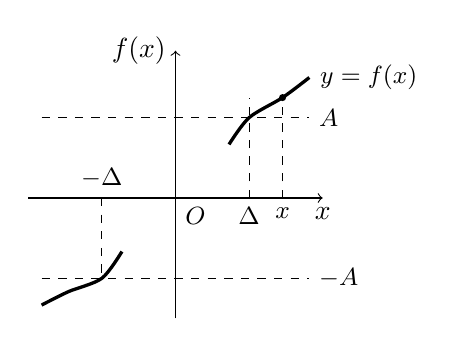
\begin{tikzpicture}[scale=0.85]
  \draw[->] (-2.2,0) -- (2.2,0) node[below] {$x$};
  \draw[->] (0,-1.8) -- (0,2.2) node[left] {$f(x)$};
  \node[below right] at (0,0) {\small $O$};
  
  \draw[dashed] (1.1,0) node[below] {\small $\Delta$} -- (1.1,1.5);
  \draw[dashed] (1.6,0) node[below] {\small $x$} -- (1.6,1.5);
  \draw[dashed] (-1.1,0) node[above] {\small $-\Delta$} -- (-1.1,-1.2);
  
  \draw[dashed] (-2,1.2) -- (2,1.2) node[right] {\small $A$};
  \draw[dashed] (-2,-1.2) -- (2,-1.2) node[right] {\small $-A$};
  
  \draw[very thick] plot [smooth] coordinates {(0.8,0.8) (1.1,1.2) (1.6,1.5) (2.0,1.8)} node[right, font=\small] {$y=f(x)$};
  \draw[very thick] plot [smooth] coordinates {(-2.0,-1.6) (-1.6,-1.4) (-1.1,-1.2) (-0.8,-0.8)};
  \fill (1.6,1.5) circle (1.5pt);
\end{tikzpicture}
\caption{}\label{fig:2.1.9}
\end{minipage}
\hfill
\begin{minipage}[t]{0.45\textwidth}
\centering
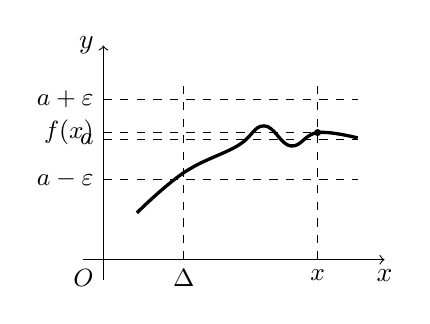
\begin{tikzpicture}[scale=0.85]
  \draw[->] (-0.3,0) -- (4.2,0) node[below] {$x$};
  \draw[->] (0,-0.3) -- (0,3.2) node[left] {$y$};
  \node[below left] at (0,0) {\small $O$};
  
  \draw[dashed] (1.2,0) node[below] {\small $\Delta$} -- (1.2,2.6);
  \draw[dashed] (3.2,0) node[below] {\small $x$} -- (3.2,2.6);
  
  \draw[dashed] (0,1.2) node[left] {\small $a-\varepsilon$} -- (3.8,1.2);
  \draw[dashed] (0,1.8) node[left] {\small $a$} -- (3.8,1.8);
  \draw[dashed] (0,2.4) node[left] {\small $a+\varepsilon$} -- (3.8,2.4);
  \draw[dashed] (0,1.9) node[left] {\small $f(x)$} -- (3.2,1.9);
  
  \draw[very thick] plot [smooth, tension=0.7] coordinates {(0.5,0.7) (1.2,1.3) (2.0,1.7) (2.4,2.0) (2.8,1.7) (3.2,1.9) (3.8,1.82)};
  \fill (3.2,1.9) circle (1.5pt);
\end{tikzpicture}
\caption{}\label{fig:2.1.10}
\end{minipage}
\end{figure}

其余 20 种情形读者自行叙述, 并配出相应的示意图.

\begin{theorem}\label{thm:2.1.1}
$\lim\limits_{x \to x_0} f(x) = a \iff f(x_0^+) = \lim\limits_{x \to x_0^+} f(x) = a = \lim\limits_{x \to x_0^-} f(x) = f(x_0^-)$, 其中 $a$ 为实数, $+\infty, -\infty, \infty$.
\end{theorem}

\begin{proof}
($\Rightarrow$) 显然.

($\Leftarrow$) 对于 $a$ 的任何开邻域 $U(a)$, 因 $\lim\limits_{x\to x_0^+}f(x)=a$, 故 $\exists\delta_1>0$, 当 $x_0<x<x_0+\delta_1$ 时, $f(x)\in U(a)$. 因为 $\lim\limits_{x\to x_0^-}f(x)=a$, 所以 $\exists\delta_2>0$, 当 $x_0-\delta_2<x<x_0$ 时, $f(x)\in U(a)$.

因此, 取 $\delta = \min\{\delta_1, \delta_2\}$, 当 $0 < |x - x_0| < \delta$ 时, 有 $f(x) \in U(a)$. 于是,
\[
\lim_{x\to x_{0}}f(x)=a.
\]
\end{proof}

\begin{theorem}\label{thm:2.1.2}
$\lim\limits_{x\to\infty}f(x)=a \iff \lim\limits_{x\to+\infty}f(x)=a$ 且 $\lim\limits_{x\to-\infty}f(x)=a$, 其中 $a$ 为实数, $+\infty, -\infty, \infty$.
\end{theorem}

\begin{proof}
($\Rightarrow$) 对 $a$ 的任何开邻域 $U(a)$, 因 $\lim\limits_{x\to\infty}f(x)=a$, 故 $\exists\Delta>0$, 当 $|x|>\Delta$ 时, 必有 $f(x)\in U(a)$. 于是, 当 $x>\Delta$ 时, 有 $f(x)\in U(a)$, 从而 $\lim\limits_{x\to+\infty}f(x)=a$; 当 $x < -\Delta$ 时, 有 $f(x) \in U(a)$, 从而 $\lim\limits_{x\to-\infty} f(x) = a$.

($\Leftarrow$) 由 $\lim\limits_{x\to+\infty}f(x)=a$, 故对 $a$ 的任何开邻域 $U(a)$, $\exists\Delta_{1}>0$, 当 $x>\Delta_{1}$ 时, 有 $f(x)\in U(a)$. 再由 $\lim\limits_{x\to-\infty}f(x)=a$, 故对 $a$ 的任何开邻域 $U(a)$, $\exists\Delta_{2}>0$, 当 $x<-\Delta_{2}$ 时, 有 $f(x)\in U(a)$. 因此当 $|x|>\Delta=\max\{\Delta_{1},\Delta_{2}\}$ 时, $f(x)\in U(a)$, 从而 $\lim\limits_{x\to\infty}f(x)=a$.
\end{proof}

\begin{theorem}[归结原则, Heine]\label{thm:2.1.3}
函数 $y = f(x)$, 其定义域为 $x_{0}$ 的去心开邻域 $U^{\circ}(x_{0})$, 则在 $U^{\circ}(x_{0})$ 中有
\[
\lim_{x\to x_0}f(x)=a \iff \forall \{x_n\}\subset U^\circ(x_0),\ x_n\to x_0\ (n\to+\infty),\text{ 必有 } \lim_{n\to+\infty}f(x_n)=a,
\]
其中 $a$ 为实数, $+\infty, -\infty, \infty$; $x_0$ 可换为 $x_0^+, x_0^-, +\infty, -\infty, \infty$.
\end{theorem}

\begin{proof}
先证 $a \in \mathbb{R}, x_0 \in \mathbb{R}$ 的情形.

($\Rightarrow$) $\forall\varepsilon>0$, 因为 $\lim\limits_{x\to x_0}f(x)=a$, 所以 $\exists\delta>0$, 当 $0<|x-x_0|<\delta$ 时, $|f(x)-a|<\varepsilon$. 而由于 $\forall x_n\neq x_0, x_n\to x_0\ (n\to+\infty)$, 所以对取定的 $\delta>0$, $\exists N\in\mathbb{N}$, 当 $n>N$ 时, 有 $0<|x_n-x_0|<\delta$, 所以
\[
|f(x_{n})-a|<\varepsilon,
\]
即 $\lim\limits_{n\to+\infty}f(x_{n})=a$.

($\Leftarrow$) (反证)假设 $\lim\limits_{x \to x_0} f(x) \neq a$, 则 $\exists \varepsilon_0 > 0, \forall n \in \mathbb{N}$, $\exists x_n \neq x_0$, s.t. $0 < |x_n - x_0| < \frac{1}{n}$, 但
\[
|f(x_{n})-a|\geqslant\varepsilon_{0}.
\]
显然, $\lim\limits_{n\to+\infty} x_{n}=x_{0}$, 但由条件知,
\[
0=|a-a|=\lim_{n\to+\infty}|f(x_{n})-a|\geqslant\varepsilon_{0}>0,
\]
矛盾. 所以, $\lim\limits_{x\to x_0}f(x)=a$.

其他情形可类似证明.

统一描述如下:

($\Rightarrow$) 对 $a$ 的任何开邻域 $U(a)$, 因为 $\lim\limits_{x \to x_0} f(x) = a$, 存在 $x_0$ 的去心开邻域 $V^\circ(x_0)$, 当 $x \in V^\circ(x_0)$ 时, $f(x) \in U(a)$. 又因 $x_n \to x_0\ (n \to +\infty), x_n \neq x_0$, 故 $\exists N \in \mathbb{N}$, 当 $n > N$ 时, $x_n \in V^\circ(x_0)$, 从而 $f(x_n) \in U(a)$. 这就证明了 $\lim\limits_{n \to +\infty} f(x_n) = a$.

($\Leftarrow$) (反证)假设 $\lim\limits_{x\to x_0}f(x)\neq a$, 则存在 $a$ 的开邻域 $U_0(a)$, $\forall n\in\mathbb{N}$, $\exists x_n\neq x_0$, s.t. $x_n\in V^\circ_n(x_0)$ (6 种情形分别为 $(x_0-\frac{1}{n},x_0+\frac{1}{n})\setminus\{x_0\}$, $(x_0,x_0+\frac{1}{n})$, $(x_0-\frac{1}{n},x_0)$, $(n,+\infty)$, $(-\infty,-n)$, $(-\infty,-n)\cup(n,+\infty)$), 但是 $f(x_n)\notin U_0(a)$. 显然, $\lim\limits_{n\to+\infty}x_n=x_0$, 但 $\lim\limits_{n\to+\infty}f(x_n)\neq a$, 这与已知条件矛盾.
\end{proof}

\begin{theorem}[函数收敛的 Cauchy 准则]\label{thm:2.1.4}
设 $f$ 在 $x_{0}$ 的去心开邻域 $U^{\circ}(x_{0},\delta_{0})$ 内定义, 则 $\lim\limits_{x\to x_0} f(x)$ 存在有限 $\iff \forall\varepsilon>0,\exists\delta\in(0,\delta_{0})$, s.t. $\forall x^{\prime},x^{\prime\prime}\in U^{\circ}(x_{0},\delta)$, 有
\[
|f(x^{\prime})-f(x^{\prime \prime})|<\varepsilon.
\]
\end{theorem}

\begin{proof}
($\Rightarrow$) 设 $\lim\limits_{x\to x_0}f(x)=a\in\mathbb{R}$, 则 $\forall\varepsilon>0,\exists\delta\in(0,\delta_0)$, s.t. $\forall x\in U^\circ(x_0,\delta)$, 有 $|f(x)-a|<\frac{\varepsilon}{2}$. 于是, 对于 $\forall x',x''\in U^\circ(x_0,\delta)$, 有
\begin{align*}
|f(x^{\prime})-f(x^{\prime \prime})| &= |(f(x^{\prime})-a)-(f(x^{\prime \prime})-a)| \\
&\leqslant |f(x^{\prime})-a|+|f(x^{\prime \prime})-a| < \frac{\varepsilon}{2}+\frac{\varepsilon}{2}=\varepsilon.
\end{align*}

($\Leftarrow$) 设数列 $\{x_n\}\subset U^\circ(x_0,\delta_0)$, 且 $\lim\limits_{n\to+\infty}x_n=x_0$. 按已知条件, $\forall\varepsilon>0$, $\exists\delta\in(0,\delta_0)$, s.t. $\forall x',x''\in U^\circ(x_0,\delta)$, 有 $|f(x')-f(x'')|<\varepsilon$.

对上述的 $\delta$, 由于 $\lim\limits_{n\to+\infty}x_n=x_0$, 故 $\exists N\in\mathbb{N}$, 当 $n,m>N$ 时, 有 $x_n,x_m\in U^\circ(x_0,\delta)$. 从而, $|f(x_n)-f(x_m)|<\varepsilon$. 这表明了 $\{f(x_n)\}$ 为 Cauchy 数列. 根据数列的 Cauchy 准则知, $\{f(x_n)\}$ 收敛.

进一步考虑 $\{x_{n}^{\prime}\}\subset U^{\circ}(x_{0},\delta_{0})$, $\{x_{n}^{\prime\prime}\}\subset U^{\circ}(x_{0},\delta_{0})$, 且 $\lim\limits_{n\to+\infty}x_{n}^{\prime}=x_{0}=\lim\limits_{n\to+\infty}x_{n}^{\prime\prime}$. 构造交错数列 $\{x_n\}\colon x_{1}^{\prime}, x_{1}^{\prime\prime}, x_{2}^{\prime}, x_{2}^{\prime\prime}, \cdots, x_{k}^{\prime}, x_{k}^{\prime\prime}, \cdots$, 显然 $\{x_{n}\}\subset U^{\circ}(x_{0},\delta_{0})$, $\lim\limits_{n\to+\infty}x_{n}=x_{0}$. 由上述证明所得结果, $\{f(x_{n})\}$ 收敛, 从而
\[
\lim_{n\to+\infty}f(x_{n}^{\prime})=\lim_{n\to+\infty}f(x_{n})=\lim_{n\to+\infty}f(x_{n}^{\prime\prime}),
\]
记此公共极限为 $a$. 根据归结原则(定理~\ref{thm:2.1.3}), $\lim\limits_{x\to x_0}f(x)=a$.
\end{proof}

\begin{remark}\label{rem:2.1.1}
定理~\ref{thm:2.1.4} 等价于: $f(x)$ 在 $x_{0}$ 不存在有限极限 $\iff \exists \varepsilon_{0} > 0, \forall \delta > 0$, 总有 $x_{\delta}^{\prime}, x_{\delta}^{\prime\prime} \in U^{\circ}(x_{0}, \delta)$, s.t. $|f(x_{\delta}^{\prime}) - f(x_{\delta}^{\prime\prime})| \geqslant \varepsilon_{0}$.
\end{remark}

\begin{remark}\label{rem:2.1.2}
定理~\ref{thm:2.1.4} 与注~\ref{rem:2.1.1} 中, $x_{0}$ 换为 $x_{0}^{\pm}, \pm\infty, \infty$, 相应结论成立, 证明也类似.
\end{remark}

\begin{example}\label{ex:2.1.4}
设 $f(x) = c$ 为常值函数, 则 $\lim\limits_{x \to x_0} f(x) = c$, 其中 $x_0$ 或 $x_0^+, x_0^-, +\infty, -\infty, \infty$.
\end{example}

\begin{proof}
$\forall\varepsilon>0$, 任取 $\delta>0$, 当 $0<|x-x_{0}|<\delta$ 时, 有
\[
|f(x)-c|=|c-c|=0<\varepsilon,
\]
所以 $\lim\limits_{x\to x_0}f(x)=c$. 其他情形类似证明.
\end{proof}

\begin{example}\label{ex:2.1.5}
证明: $\lim\limits_{x\to+\infty}\frac{1}{x^\alpha}=0\ (\alpha>0)$.
\end{example}

\begin{proof}
$\forall\varepsilon>0$, 取 $\Delta>\left(\frac{1}{\varepsilon}\right)^{\frac{1}{\alpha}}$, 则当 $x>\Delta$ 时, 有
\[
\left|\frac{1}{x^{\alpha}}-0\right|=\frac{1}{x^{\alpha}}<\frac{1}{\Delta^{\alpha}}<\varepsilon,
\]
所以 $\lim\limits_{x\to+\infty}\frac{1}{x^{\alpha}}=0$.
\end{proof}

\begin{example}\label{ex:2.1.6}
证明:
\begin{enumerate}[label=(\arabic*)]
  \item $\lim\limits_{x\to-\infty}\arctan x=-\frac{\pi}{2}$;
  \item $\lim\limits_{x \to +\infty} \arctan x = \frac{\pi}{2}$.
\end{enumerate}
\end{example}

\begin{proof}
(1) $\forall\varepsilon>0$, 取 $\Delta>\tan\left(\frac{\pi}{2}-\varepsilon\right)$, 当 $x<-\Delta$ 时, 有
\[
-\frac{\pi}{2}-\varepsilon<-\frac{\pi}{2}<\arctan x<\arctan(-\Delta)=-\left(\frac{\pi}{2}-\varepsilon\right)<-\frac{\pi}{2}+\varepsilon,
\]
因此 $\lim\limits_{x\to-\infty}\arctan x=-\frac{\pi}{2}$.

(2) $\forall\varepsilon>0$, 取 $\Delta>\tan\left(\frac{\pi}{2}-\varepsilon\right)=\cot\varepsilon$, 当 $x>\Delta$ 时, 有
\[
\frac{\pi}{2}-\varepsilon < \arctan\Delta < \arctan x < \frac{\pi}{2} < \frac{\pi}{2}+\varepsilon,
\]
所以 $\lim\limits_{x\to+\infty}\arctan x=\frac{\pi}{2}$ (如图~\ref{fig:2.1.11} 所示).
\end{proof}

\begin{figure}[htbp]
\centering
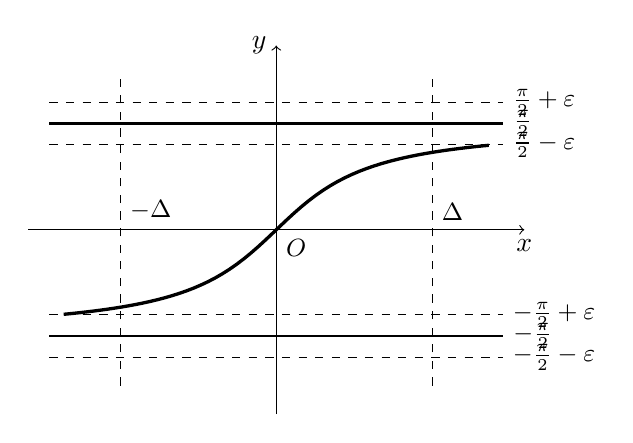
\begin{tikzpicture}[scale=0.9]
  \draw[->] (-3.5,0) -- (3.5,0) node[below] {$x$};
  \draw[->] (0,-2.6) -- (0,2.6) node[left] {$y$};
  \node[below right] at (0,0) {\small $O$};
  
  \draw[thick] (-3.2,1.5) -- (3.2,1.5) node[right] {\small $\frac{\pi}{2}$};
  \draw[thick] (-3.2,-1.5) -- (3.2,-1.5) node[right] {\small $-\frac{\pi}{2}$};
  
  \draw[dashed] (-3.2,1.8) -- (3.2,1.8) node[right] {\small $\frac{\pi}{2}+\varepsilon$};
  \draw[dashed] (-3.2,1.2) -- (3.2,1.2) node[right] {\small $\frac{\pi}{2}-\varepsilon$};
  \draw[dashed] (-3.2,-1.2) -- (3.2,-1.2) node[right] {\small $-\frac{\pi}{2}+\varepsilon$};
  \draw[dashed] (-3.2,-1.8) -- (3.2,-1.8) node[right] {\small $-\frac{\pi}{2}-\varepsilon$};
  
  \draw[dashed] (2.2,-2.2) -- (2.2,2.2);
  \node[above right] at (2.2,0) {\small $\Delta$};
  \draw[dashed] (-2.2,-2.2) -- (-2.2,2.2);
  \node[above right] at (-2.2,0) {\small $-\Delta$};
  
  \draw[very thick, domain=-3:3, samples=60] plot (\x, {1.5*(2/pi)*rad(atan(\x))});
\end{tikzpicture}
\caption{}\label{fig:2.1.11}
\end{figure}

\begin{example}\label{ex:2.1.7}
证明: $\lim\limits_{x\to2}\frac{x^{2}-4}{x-2}=\lim\limits_{x\to2}(x+2)=4$.
\end{example}

\begin{proof}
$\forall\varepsilon>0$, 取 $\delta=\varepsilon$, 当 $0<|x-2|<\delta=\varepsilon$ 时, 有
\[
\left|\frac{x^{2}-4}{x-2}-4\right|=|(x+2)-4|=|x-2|<\delta=\varepsilon,
\]
因此 $\lim\limits_{x\to2}\frac{x^{2}-4}{x-2}=4$.
\end{proof}

函数 $y=\frac{x^{2}-4}{x-2}$ 和 $y=x+2$ 的定义域不同, 前者为 $\mathbb{R}\setminus\{2\}$, 后者为 $\mathbb{R}$, 但它们在 $x\to2$ 时有相同的极限, 这是因为在考虑 $x\to x_{0}$ 的极限时, 并不要求函数在 $x=x_{0}$ 处有定义或函数在 $x_{0}$ 处的值是多少. 下面的例子也是如此.

\begin{example}\label{ex:2.1.8}
证明: $\lim\limits_{x\to1}\frac{x^{2}-1}{2x^{2}-x-1}=\lim\limits_{x\to1}\frac{x+1}{2x+1}=\frac{2}{3}$.
\end{example}

\begin{proof}
$\forall\varepsilon>0$, 取 $\delta=\min\{1,3\varepsilon\}$ (如图~\ref{fig:2.1.12} 所示), 当 $0<|x-1|<\delta$ 时, 有
\[
\left|\frac{x^2-1}{2x^2-x-1}-\frac{2}{3}\right|=\left|\frac{x+1}{2x+1}-\frac{2}{3}\right|=\frac{|x-1|}{3|2x+1|}<\frac{\delta}{3}\leqslant\varepsilon,
\]
所以 $\lim\limits_{x\to1}\frac{x^{2}-1}{2x^{2}-x-1}=\frac{2}{3}$.
\end{proof}

\begin{remark}\label{rem:2.1.3}
为了使得 $|2x+1|\geqslant1$, 我们先限制 $|x-1|<1\iff 0<x<2$. 再由 $\frac{\delta}{3}\leqslant\varepsilon$ 解得 $\delta\leqslant3\varepsilon$, 所以取 $\delta=\min\{1,3\varepsilon\}$.

如果先限制 $|x-1| < \frac{1}{2} \iff -\frac{1}{2} < x-1 < \frac{1}{2} \iff \frac{1}{2} < x < \frac{3}{2}$ (如图~\ref{fig:2.1.13} 所示). 于是, $|2x+1| \geqslant |2 \cdot \frac{1}{2}+1| = 2$, 从而
\[
\left|\frac{x^{2}-1}{2x^{2}-x-1}-\frac{2}{3}\right|=\frac{|x-1|}{3|2x+1|}<\frac{\delta}{3\cdot2}=\frac{\delta}{6}\leqslant\varepsilon,
\]
只需取 $\delta = \min\left\{\frac{1}{2},6\varepsilon\right\}$.
\end{remark}

\begin{figure}[htbp]
\centering
\begin{minipage}[t]{0.45\textwidth}
\centering
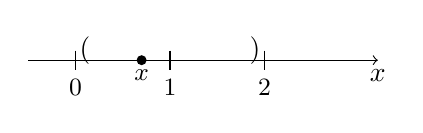
\begin{tikzpicture}[scale=1.2]
  \draw[->] (-0.5,0) -- (3.2,0) node[below] {$x$};
  \draw (0,0.1) -- (0,-0.1) node[below] {\small $0$};
  \draw (1,0.1) -- (1,-0.1) node[below] {\small $1$};
  \draw (2,0.1) -- (2,-0.1) node[below] {\small $2$};
  \node at (0.1,0.1) {$($};
  \node at (1.9,0.1) {$)$};
  \fill (0.7,0) circle (1.5pt) node[below] {\small $x$};
\end{tikzpicture}
\caption{}\label{fig:2.1.12}
\end{minipage}
\hfill
\begin{minipage}[t]{0.45\textwidth}
\centering
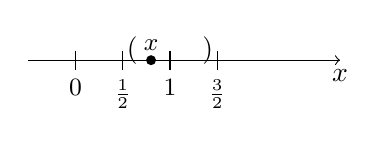
\begin{tikzpicture}[scale=1.2]
  \draw[->] (-0.5,0) -- (2.8,0) node[below] {$x$};
  \draw (0,0.1) -- (0,-0.1) node[below] {\small $0$};
  \draw (0.5,0.1) -- (0.5,-0.1) node[below] {\small $\frac{1}{2}$};
  \draw (1,0.1) -- (1,-0.1) node[below] {\small $1$};
  \draw (1.5,0.1) -- (1.5,-0.1) node[below] {\small $\frac{3}{2}$};
  \node at (0.6,0.1) {$($};
  \node at (1.4,0.1) {$)$};
  \fill (0.8,0) circle (1.5pt) node[above] {\small $x$};
\end{tikzpicture}
\caption{}\label{fig:2.1.13}
\end{minipage}
\end{figure}

\begin{example}\label{ex:2.1.9}
证明:
\begin{enumerate}[label=(\arabic*)]
  \item $\lim\limits_{x\to1^{+}}\frac{x^{2}+1}{x^{2}-1}=+\infty$;
  \item $\lim\limits_{x \to 1^-} \frac{x^2 + 1}{x^2 - 1} = -\infty$.
\end{enumerate}
\end{example}

\begin{proof}
(1) $\forall A>0$, 取 $\delta=\min\left\{1,\frac{1}{3A}\right\}$ (如图~\ref{fig:2.1.14} 所示), 当 $1<x<1+\delta$ 时, 有
\[
\frac{x^{2}+1}{x^{2}-1}=\frac{x^{2}+1}{(x+1)(x-1)}>\frac{1}{(2+1)\delta}=\frac{1}{3\delta}\geqslant A,
\]
所以 $\lim\limits_{x\to1^{+}}\frac{x^{2}+1}{x^{2}-1}=+\infty$.

(2) $\forall A>0$, 取 $\delta=\min\left\{1,\frac{1}{2A}\right\}$ (如图~\ref{fig:2.1.15} 所示), 当 $1-\delta<x<1$ 时, 有
\[
\frac{x^{2}+1}{x^{2}-1}=\frac{x^{2}+1}{(x+1)(x-1)}=-\frac{x^{2}+1}{(x+1)(1-x)}<-\frac{1}{2\delta}<-A,
\]
因此 $\lim\limits_{x\to1^{-}}\frac{x^{2}+1}{x^{2}-1}=-\infty$.
\end{proof}

\begin{figure}[htbp]
\centering
\begin{minipage}[t]{0.45\textwidth}
\centering
\begin{tikzpicture}[scale=1.2]
  \draw[->] (-0.5,0) -- (3.2,0) node[below] {$x$};
  \draw (0,0.1) -- (0,-0.1) node[below] {\small $0$};
  \draw (1,0.1) -- (1,-0.1) node[below] {\small $1$};
  \draw (2,0.1) -- (2,-0.1) node[below] {\small $2$};
  \node at (1.8,0.1) {$)$};
  \fill (1.4,0) circle (1.5pt) node[below] {\small $x$};
\end{tikzpicture}
\caption{}\label{fig:2.1.14}
\end{minipage}
\hfill
\begin{minipage}[t]{0.45\textwidth}
\centering
\begin{tikzpicture}[scale=1.2]
  \draw[->] (-0.5,0) -- (3.2,0) node[below] {$x$};
  \draw (0,0.1) -- (0,-0.1) node[below] {\small $0$};
  \draw (1,0.1) -- (1,-0.1) node[below] {\small $1$};
  \draw (2,0.1) -- (2,-0.1) node[below] {\small $2$};
  \node at (0.2,0.1) {$($};
  \fill (0.7,0) circle (1.5pt) node[below] {\small $x$};
\end{tikzpicture}
\caption{}\label{fig:2.1.15}
\end{minipage}
\end{figure}

\begin{example}\label{ex:2.1.10}
证明 $\lim\limits_{x\to0}x^{\alpha}\sin\frac{1}{x}=0\ (\alpha>0)$ (如图~\ref{fig:2.1.16} 所示).
\end{example}

\begin{proof}
$\forall\varepsilon>0$, 取 $\delta=\varepsilon^{\frac{1}{\alpha}}$, 当 $0<|x-0|<\delta$ 时, 有
\[
\left|x^{\alpha}\sin\frac{1}{x}-0\right|\leqslant|x|^{\alpha}<\delta^{\alpha}=\varepsilon,
\]
这就证明了 $\lim\limits_{x\to0}x^{\alpha}\sin\frac{1}{x}=0$.
\end{proof}

\begin{figure}[htbp]
\centering
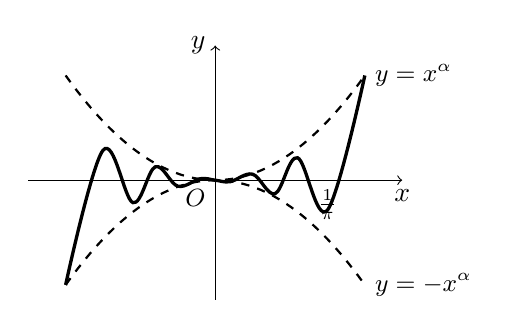
\begin{tikzpicture}[scale=0.95]
  \draw[->] (-2.5,0) -- (2.5,0) node[below] {$x$};
  \draw[->] (0,-1.6) -- (0,1.8) node[left] {$y$};
  \node[below left] at (0,0) {\small $O$};
  
  \draw[dashed, thick, domain=-2:2, samples=50] plot (\x, {0.35*\x*\x}) node[right] {\small $y=x^\alpha$};
  \draw[dashed, thick, domain=-2:2, samples=50] plot (\x, {-0.35*\x*\x}) node[right] {\small $y=-x^\alpha$};
  
  \draw[very thick] plot [smooth, tension=0.6] coordinates {
    (-2.0, -1.4) (-1.5, 0.4) (-1.1, -0.3) (-0.8, 0.18) (-0.5, -0.08) (-0.2, 0.02)
    (0,0)
    (0.2, -0.02) (0.5, 0.08) (0.8, -0.18) (1.1, 0.3) (1.5, -0.4) (2.0, 1.4)
  };
  \node[below] at (1.5,0) {\small $\frac{1}{\pi}$};
\end{tikzpicture}
\caption{}\label{fig:2.1.16}
\end{figure}

\begin{example}\label{ex:2.1.11}
设 $\lim\limits_{x\to x_0}f(x)=0, |g(x)|\leqslant M$, 则 $\lim\limits_{x\to x_0}f(x)g(x)=0$.
\end{example}

\begin{proof}
$\forall\varepsilon>0$, 因 $\lim\limits_{x\to x_0}f(x)=0$, 故 $\exists\delta>0$, 当 $0<|x-x_0|<\delta$ 时, 有 $|f(x)-0|<\frac{\varepsilon}{M+1}$. 于是,
\[
|f(x)g(x)-0|=|f(x)|\cdot|g(x)|\leqslant M|f(x)-0|<M\cdot\frac{\varepsilon}{M+1}<\varepsilon,
\]
这就证明了 $\lim\limits_{x\to x_{0}}f(x)g(x)=0$.
\end{proof}

\begin{example}\label{ex:2.1.12}
设
\[
f(x)=\begin{cases}
1, & x<0, \\
x\sin\frac{1}{x}, & x>0.
\end{cases}
\]
证明: $\lim\limits_{x\to0}f(x)$ 不存在.
\end{example}

\begin{proof}
因为
\begin{align*}
f(0+0) &= f(0^{+})=\lim_{x\to0^{+}}x\sin\frac{1}{x}=0, \\
f(0-0) &= f(0^{-})=\lim_{x\to0^{-}}f(x)=\lim_{x\to0^{-}}1=1,
\end{align*}
$f(0^{+})\neq f(0^{-})$, 所以根据定理~\ref{thm:2.1.1} 知, $\lim\limits_{x\to0}f(x)$ 不存在.
\end{proof}

\begin{example}\label{ex:2.1.13}
证明: 符号函数 $\operatorname{sgn} x$ 在 $x=0$ 处无极限.
\end{example}

\begin{proof}
因为
\[
\operatorname{sgn}(0^{+})=\lim_{x\to0^{+}}\operatorname{sgn} x=\lim_{x\to0^{+}}1=1\neq-1=\lim_{x\to0^{-}}(-1)=\lim_{x\to0^{-}}\operatorname{sgn} x=\operatorname{sgn}(0^{-}),
\]
所以根据定理~\ref{thm:2.1.1} 知, $\operatorname{sgn} x$ 在 $x=0$ 处无极限.
\end{proof}

\begin{example}\label{ex:2.1.14}
证明 $\lim\limits_{x\to0}\sin\frac{1}{x}$ 不存在.
\end{example}

\begin{proof}
取数列 $x_{n}^{\prime}=\frac{1}{2n\pi}\to0\ (n\to+\infty)$, $x_{n}^{\prime\prime}=\frac{1}{2n\pi+\frac{\pi}{2}}\to0\ (n\to+\infty)$. 显然,
\begin{align*}
\lim_{n\to+\infty}\sin\frac{1}{x_{n}^{\prime}} &= \lim_{n\to+\infty}\sin 2n\pi = 0, \\
\lim_{n\to+\infty}\sin\frac{1}{x_{n}^{\prime\prime}} &= \lim_{n\to+\infty}\sin\left(2n\pi+\frac{\pi}{2}\right) = 1,
\end{align*}
$\lim\limits_{n\to+\infty}\sin\frac{1}{x_{n}^{\prime}}\neq\lim\limits_{n\to+\infty}\sin\frac{1}{x_{n}^{\prime\prime}}$. 所以根据定理~\ref{thm:2.1.3} 知, $\lim\limits_{x\to0}\sin\frac{1}{x}$ 不存在(如图~\ref{fig:2.1.17} 所示).
\end{proof}

\begin{figure}[htbp]
\centering
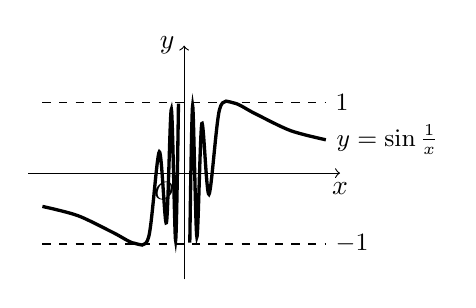
\begin{tikzpicture}[scale=0.9]
  \draw[->] (-2.2,0) -- (2.2,0) node[below] {$x$};
  \draw[->] (0,-1.5) -- (0,1.8) node[left] {$y$};
  \node[below left] at (0,0) {\small $O$};
  
  \draw[dashed] (-2,1) -- (2,1) node[right] {\small $1$};
  \draw[dashed] (-2,-1) -- (2,-1) node[right] {\small $-1$};
  
  \draw[very thick] plot [smooth, tension=0.5] coordinates {
    (-2.0,-0.47) (-1.5,-0.6) (-1.0,-0.84) (-0.7,-0.99) (-0.5,-0.9)
    (-0.35, 0.3) (-0.25, -0.7) (-0.18, 0.9) (-0.12, -0.95) (-0.08, 0.98)
  };
  \draw[very thick] plot [smooth, tension=0.5] coordinates {
    (0.08, -0.98) (0.12, 0.95) (0.18, -0.9) (0.25, 0.7) (0.35, -0.3)
    (0.5, 0.9) (0.7, 0.99) (1.0, 0.84) (1.5, 0.6) (2.0, 0.47)
  } node[right, font=\small] {$y=\sin\frac{1}{x}$};
\end{tikzpicture}
\caption{}\label{fig:2.1.17}
\end{figure}

\begin{example}\label{ex:2.1.15}
证明 Dirichlet 函数
\[
D(x)=\begin{cases}
1, & x\in\mathbb{Q}, \\
0, & x\in\mathbb{R}\setminus\mathbb{Q}
\end{cases}
\]
在任何点处无极限.
\end{example}

\begin{proof}
\textit{证法 1}\quad $\forall x_0 \in \mathbb{R}$, 取 $x'_n \in \mathbb{Q}, x'_n \neq x_0, x'_n \to x_0\ (n \to +\infty)$; 再取 $x''_n \in \mathbb{R} \setminus \mathbb{Q}, x''_n \neq x_0, x''_n \to x_0\ (n \to +\infty)$, 则
\[
\lim_{n\to+\infty}D(x_{n}^{\prime})=\lim_{n\to+\infty}1=1,\quad \lim_{n\to+\infty}D(x_{n}^{\prime \prime})=\lim_{n\to+\infty}0=0.
\]
因为 $\lim\limits_{n\to+\infty}D(x_{n}^{\prime})\neq\lim\limits_{n\to+\infty}D(x_{n}^{\prime\prime})$, 所以根据定理~\ref{thm:2.1.3} 知, $\lim\limits_{x\to x_{0}}D(x)$ 不存在.

\textit{证法 2}\quad (反证)反设在点 $x_{0} \in \mathbb{R}$, $\lim\limits_{x \to x_{0}} D(x) = a$, 则 $0$ 与 $1$ 中至少有一个不为 $a$. 不妨设 $a \neq 1$, 则存在 $a$ 的开邻域 $U(a) \not\ni 1$. 于是, $\exists \delta > 0$, 当 $0 < |x - x_{0}| < \delta$ 时, $D(x) \in U(a)$, 当然 $D(x) \neq 1$. 但因 $\mathbb{Q}$ 在 $\mathbb{R}$ 中是稠密的, 必有 $x' \in \mathbb{Q}$, s.t. $0 < |x' - x_{0}| < \delta$, 所以 $1=D(x^{\prime})\in U(a)$, 这与 $1 \notin U(a)$ 相矛盾.
\end{proof}

\begin{example}\label{ex:2.1.16}
证明:
\[
\lim_{x\to+\infty}a^x=\begin{cases}
+\infty, & a>1, \\
1, & a=1, \\
0, & 0<a<1.
\end{cases}
\]
\end{example}

\begin{proof}
当 $a>1$ 时, $\forall A>0$, 取 $\Delta>\log_{a}A$. 当 $x>\Delta$ 时, 有
\[
a^{x}>a^{\Delta}>A,
\]
所以 $\lim\limits_{x\to+\infty}a^{x}=+\infty$.

当 $0 < a < 1$ 时, $\forall \varepsilon > 0$, 取 $\Delta > \log_{a}\varepsilon$. 当 $x > \Delta$ 时, 有
\[
|a^{x}-0|=a^{x}<a^{\Delta}<\varepsilon,
\]
所以 $\lim\limits_{x\to+\infty}a^{x}=0$.

当 $a=1$ 时, $\lim\limits_{x\to+\infty}a^{x}=\lim\limits_{x\to+\infty}1^{x}=\lim\limits_{x\to+\infty}1=1$.
\end{proof}

\begin{example}\label{ex:2.1.17}
证明:
\begin{enumerate}[label=(\arabic*)]
  \item $\lim\limits_{x\to 0}a^{x}=1\ (a>0)$;
  \item $\lim\limits_{x \to 1} \log_a x = 0\ (a > 0, a \neq 1)$.
\end{enumerate}
\end{example}

\begin{proof}
(1) 设 $a=1$, 显然 $\lim\limits_{x\to0}a^{x}=\lim\limits_{x\to0}1^{x}=1$.

设 $a>1$. $\forall\varepsilon\in(0,1)$, 取 $\delta=\min\{|\log_{a}(1-\varepsilon)|,|\log_{a}(1+\varepsilon)|\}$, 当 $0<|x-0|=|x|<\delta$ 时, 有
\[
\log_{a}(1-\varepsilon)<x<\log_{a}(1+\varepsilon)\implies 1-\varepsilon<a^{x}<1+\varepsilon\implies |a^{x}-1|<\varepsilon,
\]
所以 $\lim\limits_{x\to0} a^x = 1$.

设 $0 < a < 1$. $\forall \varepsilon \in (0,1)$, 取 $\delta = \min\{|\log_{a}(1-\varepsilon)|, |\log_{a}(1+\varepsilon)|\}$, 当 $0 < |x| < \delta$ 时, 有
\[
\log_{a}(1+\varepsilon)<x<\log_{a}(1-\varepsilon)\implies 1-\varepsilon<a^{x}<1+\varepsilon\implies |a^{x}-1|<\varepsilon,
\]
所以 $\lim\limits_{x\to0}a^{x}=1$.

(2) 不失一般性, 设 $a > 1$. $\forall \varepsilon > 0$, 必存在 $\varepsilon_{1} > 0$, 使得 $a^{-\varepsilon} < 1 - \varepsilon_{1} < 1 + \varepsilon_{1} < a^{\varepsilon}$. 当 $a^{-\varepsilon}<1-\varepsilon_{1}<x<1+\varepsilon_{1}<a^{\varepsilon}$ 时, 有
\[
-\varepsilon<\log_{a}x<\varepsilon\implies |\log_{a}x-0|<\varepsilon,
\]
故 $\lim\limits_{x\to1}\log_{a}x=0$.
\end{proof}

\begin{lemma}\label{lem:2.1.1}
证明:
\begin{enumerate}[label=(\arabic*)]
  \item $\sin x < x < \tan x,\ 0 < x < \frac{\pi}{2}$;
  \item $\sin x < x,\ \forall x \in (0, +\infty)$;
  \item $|\sin x|\leqslant|x|,\ \forall x\in\mathbb{R}$.
\end{enumerate}
\end{lemma}

\begin{proof}
(1) 图~\ref{fig:2.1.18} 所示是一单位圆, 用 $S_{\triangle OCD}, S_{\text{扇形}OAD}, S_{\triangle OAB}$ 分别表示 $\triangle OCD$, 扇形 $OAD$ 和 $\triangle OAB$ 的面积. 显然,
\[
S_{\triangle OCD}<S_{\text{扇形}OAD}<S_{\triangle OAB},
\]
从而 $\frac{1}{2}\sin x\cos x < \frac{1}{2}x < \frac{1}{2}\tan x$, 于是 $\sin x<x<\tan x\ (0<x<\frac{\pi}{2})$.

\begin{figure}[htbp]
\centering
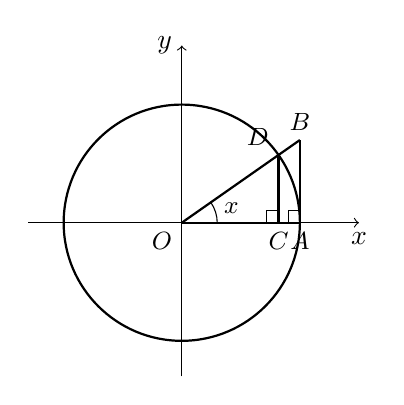
\begin{tikzpicture}[scale=1.5]
  \draw[->] (-1.3,0) -- (1.5,0) node[below] {$x$};
  \draw[->] (0,-1.3) -- (0,1.5) node[left] {$y$};
  \node[below left] at (0,0) {\small $O$};
  
  \draw[thick] (0,0) circle (1cm);
  
  \coordinate (O) at (0,0);
  \coordinate (A) at (1,0);
  \coordinate (D) at ({cos(35)}, {sin(35)});
  \coordinate (C) at ({cos(35)}, 0);
  \coordinate (B) at (1, {tan(35)});
  
  \draw[thick] (O) -- (B);
  \draw[thick] (A) -- (B);
  \draw[thick] (C) -- (D);
  \draw[thick] (O) -- (A);
  
  \node[below] at (A) {\small $A$};
  \node[above] at (B) {\small $B$};
  \node[above left] at (D) {\small $D$};
  \node[below] at (C) {\small $C$};
  
  \draw (0.3,0) arc (0:35:0.3);
  \node at (0.42,0.12) {\small $x$};
  
  \draw (0.9,0) -- (0.9,0.1) -- (1,0.1);
  \draw ({cos(35)},0.1) -- ({cos(35)-0.1},0.1) -- ({cos(35)-0.1},0);
\end{tikzpicture}
\caption{}\label{fig:2.1.18}
\end{figure}

(2) 当 $x \geqslant \frac{\pi}{2}$ 时, $x \geqslant \frac{\pi}{2} > 1 \geqslant \sin x$, 因此 $\sin x<x,\ \forall x\in(0,+\infty)$.

当 $x<0$ 时, $|\sin x|=|\sin(-x)|<-x=|x|$. 结合 $x=0$ 处等号成立, 故 $|\sin x|\leqslant|x|,\ \forall x\in\mathbb{R}$.
\end{proof}

\begin{example}\label{ex:2.1.18}
证明:
\begin{enumerate}[label=(\arabic*)]
  \item $\lim\limits_{x \to x_0} \sin x = \sin x_0$;
  \item $\lim\limits_{x \to x_0} \cos x = \cos x_0\ (x_0 \in \mathbb{R})$.
\end{enumerate}
\end{example}

\begin{proof}
(1) $\forall\varepsilon>0$, 取 $\delta=\varepsilon$, 当 $|x-x_{0}|<\delta$ 时, 由和差化积公式与引理~\ref{lem:2.1.1} 有
\[
|\sin x-\sin x_{0}|=2\left|\cos\frac{x+x_{0}}{2}\right|\left|\sin\frac{x-x_{0}}{2}\right|\leqslant2\left|\frac{x-x_{0}}{2}\right|=|x-x_{0}|<\delta=\varepsilon,
\]
所以 $\lim\limits_{x\to x_0}\sin x=\sin x_0$.

(2) 同理, $\forall\varepsilon>0$, 取 $\delta=\varepsilon$, 当 $|x-x_{0}|<\delta$ 时, 有
\[
|\cos x-\cos x_{0}|=2\left|\sin\frac{x+x_{0}}{2}\right|\left|\sin\frac{x-x_{0}}{2}\right|\leqslant2\left|\frac{x-x_{0}}{2}\right|<\delta=\varepsilon,
\]
所以 $\lim\limits_{x\to x_0}\cos x=\cos x_0$. 或由 $\lim\limits_{x\to x_0}\cos x=\lim\limits_{x\to x_0}\sin\left(\frac{\pi}{2}-x\right)=\sin\left(\frac{\pi}{2}-x_0\right)=\cos x_0$.
\end{proof}

\begin{example}\label{ex:2.1.19}
证明: $\lim\limits_{x\to x_0}\sqrt{x}=\sqrt{x_0}\ (x_0\geqslant0)$.
\end{example}

\begin{proof}
当 $x_{0}=0$ 时, $\forall\varepsilon>0$, 取 $\delta=\varepsilon^{2}$, 当 $0<x<\delta$ 时, 有
\[
|\sqrt{x}-\sqrt{0}|=\sqrt{x}<\sqrt{\delta}=\varepsilon,
\]
故 $\lim\limits_{x\to0^{+}}\sqrt{x}=0$.

当 $x_{0}>0$ 时, 取 $\delta=\min\{x_{0},\sqrt{x_{0}}\varepsilon\}$, 当 $|x-x_{0}|<\delta$ 时, 有
\[
|\sqrt{x}-\sqrt{x_{0}}|=\frac{|x-x_{0}|}{\sqrt{x}+\sqrt{x_{0}}}\leqslant\frac{|x-x_{0}|}{\sqrt{x_{0}}}<\frac{\delta}{\sqrt{x_{0}}}\leqslant\varepsilon,
\]
所以 $\lim\limits_{x\to x_0}\sqrt{x}=\sqrt{x_0}$.
\end{proof}

\begin{example}\label{ex:2.1.20}
证明: $\lim\limits_{x\to\infty}\sqrt{\frac{x^{2}+1}{x^{2}-1}}=1$.
\end{example}

\begin{proof}
\textit{证法 1}\quad $\forall\varepsilon>0$, 取 $\Delta>\max\left\{\sqrt{2},\frac{2}{\varepsilon}\right\}$, 当 $|x|>\Delta$ 时, 有
\begin{align*}
\left|\sqrt{\frac{x^2+1}{x^2-1}}-1\right| &= \left|\frac{\sqrt{x^2+1}-\sqrt{x^2-1}}{\sqrt{x^2-1}}\right|=\frac{2}{\sqrt{x^2-1}(\sqrt{x^2+1}+\sqrt{x^2-1})} \\
&< \frac{2}{x^2-1} \leqslant \frac{2}{\frac{1}{2}x^2} = \frac{4}{x^2} < \varepsilon,
\end{align*}
或放大为 $\frac{2}{|x|} < \frac{2}{\Delta} < \varepsilon$. 所以 $\lim\limits_{x\to\infty}\sqrt{\frac{x^{2}+1}{x^{2}-1}}=1$.

\textit{证法 2}\quad 变形为
\[
\lim_{x\to\infty}\sqrt{\frac{x^{2}+1}{x^{2}-1}}=\lim_{x\to\infty}\sqrt{\frac{1+\frac{1}{x^{2}}}{1-\frac{1}{x^{2}}}}=\sqrt{\frac{1+0}{1-0}}=1.
\]
\end{proof}

\begin{exblock}{练习题 2.1}
  \item 在定义~\ref{def:2.1.3} 中就 24 种情形给出函数极限的定义, 并配出相应的图形.
  \item 按函数极限的定义证明:
  \begin{enumerate}[label=(\arabic*)]
    \item $\lim\limits_{x \to +\infty} \frac{6x + 5}{x} = 6$;
    \item $\lim\limits_{x \to 2} (x^2 - 6x + 10) = 2$;
    \item $\lim\limits_{x \to +\infty} \frac{x^2 - 5}{x^2 - 1} = 1$;
    \item $\lim\limits_{x \to 2^-} \sqrt{4 - x^2} = 0$;
    \item $\lim\limits_{x \to 1} \frac{x^4 - 1}{x - 1} = 4$;
    \item $\lim\limits_{x \to 3} \frac{x - 3}{x^2 - 9} = \frac{1}{6}$;
    \item $\lim\limits_{x\to1^{+}}\frac{x-1}{\sqrt{x^{2}-1}}=0$;
    \item $\lim\limits_{x \to +\infty} (\sqrt{x+1} - \sqrt{x-1}) = 0$;
    \item $\lim\limits_{x \to \infty} \sqrt{\frac{x^2 + 2}{x^2 - 2}} = 1$.
  \end{enumerate}
  \item 设 $\lim\limits_{x \to x_0} f(x) = a$. 用 $\varepsilon - \delta$ 法证明:
  \begin{enumerate}[label=(\arabic*)]
    \item $\lim\limits_{x \to x_0} f^2(x) = a^2$;
    \item $\lim\limits_{x \to x_0} \sqrt{f(x)} = \sqrt{a}\ (a > 0)$;
    \item $\lim\limits_{x \to x_0} \sqrt[3]{f(x)} = \sqrt[3]{a}$.
  \end{enumerate}
  \item 设 $\lim\limits_{x \to x_0} f(x) = a$. 证明: $\lim\limits_{x \to x_0} |f(x)| = |a|$. 举例说明反之不成立. 问: 当且仅当 $a$ 为何值时反之也成立?
  \item 讨论下列函数在点 $0$ 处的极限或左、右极限:
  \begin{enumerate}[label=(\arabic*)]
    \item $f(x)=\frac{|x|}{x}$;
    \item $f(x)=[x]$;
    \item $f(x)=\begin{cases} 2^{x}, & x>0, \\ 0, & x=0, \\ 1+x^{2}, & x<0. \end{cases}$
  \end{enumerate}
  \item 设 $f(x)=\begin{cases} x^{2}, & x\geqslant2, \\ -ax, & x<2. \end{cases}$
  \begin{enumerate}[label=(\arabic*)]
    \item 求 $f(2^{+}), f(2^{-})$;
    \item 若 $\lim\limits_{x\to2}f(x)$ 存在, $a$ 应为何值.
  \end{enumerate}
  \item 设 $f(x_{0}^{-}) < f(x_{0}^{+})$. 证明: $\exists\delta > 0$, s.t. 当 $x_{0} - \delta < x < x_{0} < y < x_{0} + \delta$ 时, 有 $f(x) < f(y)$.
  \item 设 $f$ 在 $(-\infty, x_0)$ 内单调增, 且有一数列 $\{x_n\}$, 适合 $x_n < x_0\ (n \in \mathbb{N})$, $x_n \to x_0^-$ 及 $\lim\limits_{n \to +\infty} f(x_n) = a$. 证明: $f(x_0^-) = a = \sup\limits_{x \in U_-(x_0)} f(x)$.
  \item 用肯定的语气表述 $\lim\limits_{x \to x_{0}} f(x) \neq a$.
  \item $\forall n \in \mathbb{N}, A_n \subset [0,1]$ 为有限集, 且 $A_i \cap A_j = \varnothing\ (i \neq j), i, j \in \mathbb{N}$. 定义函数
  \[
  f(x)=\begin{cases}
  \frac{1}{n}, & x\in A_{n}, \\
  0, & x\in[0,1]\setminus\bigcup\limits_{n=1}^{\infty}A_{n}.
\end{cases}
\]
  对 $\forall x_0\in[0,1]$, 求 $\lim\limits_{x\to x_0}f(x)$.
  \item 叙述函数极限 $\lim\limits_{x \to +\infty} f(x)$ 的归结原则, 并应用它证明: $\lim\limits_{x \to +\infty} \sin x$ 与 $\lim\limits_{x \to +\infty} \cos x$ 都不存在.
  \item \begin{enumerate}[label=(\arabic*)]
    \item 叙述极限 $\lim\limits_{x \to +\infty} f(x)$ 的 Cauchy 准则;
    \item 根据 Cauchy 准则叙述 $\lim\limits_{x \to +\infty} f(x)$ 不存在的充要条件, 并应用它证明 $\lim\limits_{x \to +\infty} \sin x$ 与 $\lim\limits_{x \to +\infty} \cos x$ 不存在.
  \item 设 $f$ 为周期函数, 且 $\lim\limits_{x\to+\infty}f(x)=0$. 证明: $f(x)\equiv0$.
  \item 设 $f$ 在 $U^{\circ}(x_{0})$ 内有定义. 证明: 若对 $\forall \{x_{n}\} \subseteq U^{\circ}(x_{0})$ 且 $\lim\limits_{n\to+\infty}x_{n}=x_{0}$, 极限 $\lim\limits_{n\to+\infty}f(x_{n})$ 都存在(实数, 或 $+\infty$, 或 $-\infty$), 则所有这些极限都相等.
  \item 设 $f$ 为定义在 $[a, +\infty)$ 上的增(减)函数. 证明: $\lim\limits_{x \to +\infty} f(x)$ 存在有限的充要条件是 $f$ 在 $[a, +\infty)$ 上有上(下)界.
  \item 设 $f$ 为 $U^{\circ}(x_{0})$ 上的单调增函数, 证明: $f(x_{0}^{-})$ 与 $f(x_{0}^{+})$ 均存在且有限, 且
  \[
  f(x_{0}^{-})=\sup_{x\in U_{-}^{\circ}(x_{0})}f(x),\quad f(x_{0}^{+})=\inf_{x\in U_{+}^{\circ}(x_{0})}f(x).
\]
\end{enumerate}
\end{exblock}

\begin{exblock}{思考题 2.1}
  \item \begin{enumerate}[label=(\arabic*)]
    \item 设函数 $f$ 在 $(0, +\infty)$ 上满足方程 $f(2x) = f(x)$, 且 $\lim\limits_{x \to +\infty} f(x) = a$. 证明: $f(x) \equiv a$.
    \item 设函数 $f$ 在 $(0, +\infty)$ 上满足方程 $f(x^{2}) = f(x)$, 且
    \[
    \lim_{x\to0^{+}}f(x)=\lim_{x\to+\infty}f(x)=f(1).
\]
    证明: $f(x) \equiv f(1), x \in (0, +\infty)$.
  \item 设函数 $f\colon (a, +\infty) \to \mathbb{R}$ 在任意有限区间 $(a, b)$ 内有界, 且
  \[
  \lim_{x\to+\infty}\left[f(x+1)-f(x)\right]=A.
\]
  证明: $\lim\limits_{x\to+\infty}\frac{f(x)}{x}=A$.
  \item 设 $a > 1, b > 1$ 为两个常数, 函数 $f\colon \mathbb{R} \to \mathbb{R}$ 在 $x = 0$ 的近旁有界, 且 $\forall x \in \mathbb{R}$, 有 $f(ax) = bf(x)$. 证明: $\lim\limits_{x \to 0} f(x) = f(0)$.
\end{enumerate}
\end{exblock}

% ====================================================================
%  徐森林、薛春华《数学分析》（第一册）
%  \S2.2  函数极限的性质
%  源：原书印刷页 99-115（PDF 物理页 105-121）
%  约定：全西文半角标点；单一落盘出口 write_tex；display 数学环境无空行；
%        原生 TikZ 矢量制图；定理/定义/例/练习题/思考题全量高保真收录
% ====================================================================
\section{函数极限的性质}\label{sec:2.2}

与数列极限一样, 函数极限有惟一性定理、局部有界性、局部保号性、保不等式性、夹逼定理、极限的四则运算法则. 此外, 还有复合函数求极限的定理. 这些性质对求函数的极限又有很大的作用.

\begin{theorem}[极限的惟一性]\label{thm:2.2.1}
如果函数 $f(x)$ 在 $x_{0}(x_{0}^{\pm},\allowbreak \pm\infty, \infty)$ 处有极限 $a$ (实数、 $+\infty,\allowbreak -\infty$), 则极限惟一.
\end{theorem}

\begin{proof}
\textit{证法 1}\quad 设 $a, b \in \mathbb{R}$ 都为 $f(x)$ 当 $x \to x_0$ 时的极限, 则 $\forall \varepsilon > 0$,
\[
\exists\,\delta_{1}>0,\text{ s.t. 当 } 0<|x-x_{0}|<\delta_{1} \text{ 时, 有 } |f(x)-a|<\frac{\varepsilon}{2},
\]
\[
\exists\,\delta_{2}>0,\text{ s.t. 当 } 0<|x-x_{0}|<\delta_{2} \text{ 时, 有 } |f(x)-b|<\frac{\varepsilon}{2}.
\]
于是, 当 $0<|x-x_0|<\delta=\min\{\delta_1,\delta_2\}$ 时, 有
\begin{align*}
0\leqslant |a-b| &= |(f(x)-a)-(f(x)-b)| \\
&\leqslant |f(x)-a|+|f(x)-b| < \frac{\varepsilon}{2}+\frac{\varepsilon}{2}=\varepsilon.
\end{align*}
令 $\varepsilon \to 0^{+}$, 得到 $0 \leqslant |a - b| \leqslant 0$, 故 $|a - b| = 0$, 即 $a = b$.

此证法不能推广到其他情形.

\textit{证法 2 (反证法)}\quad 反设 $f(x)$ 在 $x_{0}$ 处有两个不同的极限 $a, b$ ($a \neq b$). 取 $a$ 的开邻域 $V(a)$, $b$ 的开邻域 $V(b)$, 使得 $V(a) \cap V(b) = \varnothing$. 于是, 存在 $x_{0}$ 的去心开邻域 $U_{1}^{\circ}(x_{0})$, 当 $x \in U_{1}^{\circ}(x_{0})$ 时, $f(x) \in V(a)$; 存在 $x_{0}$ 的去心开邻域 $U_{2}^{\circ}(x_{0})$, 当 $x \in U_{2}^{\circ}(x_{0})$ 时, 有 $f(x) \in V(b)$. 因此, 当 $x \in U_{1}^{\circ}(x_{0}) \cap U_{2}^{\circ}(x_{0})$ 时, 有
\[
f(x)\in V(a)\cap V(b)=\varnothing,
\]
矛盾.
\end{proof}

\begin{definition}\label{def:2.2.1}
设 $f: X \to \mathbb{R}$ 为实值函数. 如果存在 $M \geqslant 0$, s.t. $|f(x)| \leqslant M$, $\forall x \in X$, 则称 $f(x)$ 在 $X$ 上有界; 如果存在 $B \in \mathbb{R}$, s.t. $f(x) \leqslant B$, $\forall x \in X$, 则称 $f(x)$ 在 $X$ 上有上界; 如果存在 $A \in \mathbb{R}$, s.t. $f(x) \geqslant A$, $\forall x \in X$, 则称 $f(x)$ 在 $X$ 上有下界 $A$. 显然,
\[
f(x) \text{ 在 } X \text{ 上有界} \iff f(x) \text{ 在 } X \text{ 上既有上界又有下界}.
\]
如: $|\sin x|\leqslant 1$, $\forall x\in\mathbb{R}$, 故 $\sin x$ 在 $\mathbb{R}$ 上有界; $e^{x}>0$, 故有下界 $0$, 但它无上界.
\end{definition}

\begin{theorem}[局部有界性]\label{thm:2.2.2}
如果 $f(x)$ 在 $x_{0}(x_{0}^{\pm}, \pm\infty, \infty)$ 处有有限极限, 则 $f(x)$ 在 $x_{0}(x_{0}^{\pm},\allowbreak \pm\infty,\allowbreak \infty)$ 的某去心开邻域 (附近) 中有界.
\end{theorem}

\begin{proof}
设 $\lim\limits_{x \to x_0} f(x) = a \in \mathbb{R}$, 取 $\varepsilon_0 = 1$, 则有 $x_0$ 的去心开邻域 $U^\circ(x_0)$, 当 $x \in U^\circ(x_0)$ 时, 有
\[
|f(x)-a|<\varepsilon_{0}=1,
\]
所以
\[
|f(x)|=|(f(x)-a)+a|\leqslant|f(x)-a|+|a|<1+|a|.
\]
这就证明了 $f(x)$ 在 $x_{0}$ 的去心开邻域 $U^{\circ}(x_{0})$ 中有界.
\end{proof}

\begin{theorem}[局部保号性]\label{thm:2.2.3}
设 $f(x)$ 在 $x_{0}(x_{0}^{\pm}, \pm\infty, \infty)$ 处有有限极限 $a > 0$ (或 $<0$), 则 $\forall r \in (0, a)$ (或 $r \in (a, 0)$), 存在 $x_{0}$ 的去心开邻域 $U^{\circ}(x_{0})$, s.t. $\forall x \in U^{\circ}(x_{0})$ 有
\[
f(x)>r>0 \quad (\text{或 } f(x)<r<0).
\]
\end{theorem}

\begin{proof}
设 $a > 0$, $\forall r \in (0, a)$, 令 $\varepsilon = a - r > 0$. 由 $\lim\limits_{x \to x_0} f(x) = a$, 故存在 $x_0$ 的去心开邻域 $U^\circ(x_0)$, 当 $x \in U^\circ(x_0)$ 时, 有
\[
f(x)>a-\varepsilon=a-(a-r)=r>0.
\]
$a<0$ 的情形可类似证明, 或用 $-f(x)$ 代替 $f(x)$.
\end{proof}

\begin{theorem}[保不等式性]\label{thm:2.2.4}
设 $f(x), g(x)$ 在 $x_{0}(x_{0}^{\pm}, \pm\infty, \infty)$ 均有极限 (实数, $+\infty, -\infty$), 且在 $x_{0}$ 的去心开邻域 $U^{\circ}(x_{0})$ 内有 $f(x) \leqslant g(x)$, 则
\[
\lim_{x\to x_{0}}f(x)\leqslant\lim_{x\to x_{0}}g(x).
\]
\end{theorem}

\begin{proof}
\textit{证法 1}\quad 设 $\lim\limits_{x \to x_0} f(x) = a \in \mathbb{R}$, $\lim\limits_{x \to x_0} g(x) = b \in \mathbb{R}$, 则 $\forall \varepsilon > 0$, 存在 $x_0$ 的去心开邻域 $U_1^\circ(x_0) \subset U^\circ(x_0)$, 当 $x \in U_1^\circ(x_0)$ 时, 有 $a - \varepsilon < f(x)$; 存在 $x_0$ 的去心开邻域 $U_2^\circ(x_0) \subset U^\circ(x_0)$, 当 $x \in U_2^\circ(x_0)$ 时有 $g(x) < b + \varepsilon$. 因此当 $x \in U_1^\circ(x_0) \cap U_2^\circ(x_0)$ 时, 有
\[
a-\varepsilon<f(x)\leqslant g(x)<b+\varepsilon,
\]
所以 $a < b + 2\varepsilon$. 令 $\varepsilon \to 0^{+}$, 得到 $a \leqslant b$.

其他情形为 $\lim\limits_{x \to x_0} f(x) = -\infty \leqslant \lim\limits_{x \to x_0} g(x)$; $\lim\limits_{x \to x_0} f(x) = +\infty = \lim\limits_{x \to x_0} g(x)$; $\lim\limits_{x \to x_0} f(x) = -\infty = \lim\limits_{x \to x_0} g(x)$; 以及 $\lim\limits_{x \to x_0} f(x) \leqslant +\infty = \lim\limits_{x \to x_0} g(x)$.

\textit{证法 2 (反证法)}\quad 反设 $\lim\limits_{x\to x_{0}}f(x)=a>b=\lim\limits_{x\to x_{0}}g(x)$, 则存在 $a$ 的开邻域 $V(a)$ 以及 $b$ 的开邻域 $V(b)$, s.t. $V(a)\cap V(b)=\varnothing$. 于是, 存在 $x_{0}$ 的去心开邻域 $U_{1}^{\circ}(x_{0})\subset U^{\circ}(x_{0})$, 当 $x\in U_{1}^{\circ}(x_{0})$ 时, 有 $f(x)\in V(a)$; 存在 $x_{0}$ 的去心开邻域 $U_{2}^{\circ}(x_{0})\subset U^{\circ}(x_{0})$, 当 $x\in U_{2}^{\circ}(x_{0})$ 时, 有 $g(x)\in V(b)$. 则当 $x\in U_{1}^{\circ}(x_{0})\cap U_{2}^{\circ}(x_{0})=U_{3}^{\circ}(x_{0})$, 有
\[
g(x)<f(x).
\]
这与已知 $f(x) \leqslant g(x)$ 相矛盾.
\end{proof}

\begin{theorem}[夹逼定理]\label{thm:2.2.5}
设 $f(x), g(x)$ 在 $x_{0}(x_{0}^{\pm}, \pm\infty, \infty)$ 有极限 $a$ (实数, $+\infty, -\infty$), 且在 $x_{0}$ 某去心开邻域 $U^{\circ}(x_{0})$ 内有
\[
f(x)\leqslant h(x)\leqslant g(x),
\]
那么
\[
\lim_{x\to x_{0}}h(x)=a.
\]
\end{theorem}

\begin{proof}
\textit{证法 1}\quad 当 $x_{0}\in\mathbb{R}, a\in\mathbb{R}, U^{\circ}(x_{0})=U^{\circ}(x_{0},\delta_{0})$ 时, $\forall\varepsilon>0$, 由 $\lim\limits_{x\to x_{0}}f(x)=\lim\limits_{x\to x_{0}}g(x)=a$, 可知:
\begin{align*}
\exists\,\delta_1 \in (0, \delta_0),&\text{ 当 } 0 < |x - x_0| < \delta_1 \text{ 时, 有 } a - \varepsilon < f(x); \\
\exists\,\delta_{2}\in(0,\delta_{0}),&\text{ 当 } 0<|x-x_{0}|<\delta_{2} \text{ 时, 有 } g(x)<a+\varepsilon.
\end{align*}
于是, 当 $0<|x-x_0|<\delta=\min\{\delta_1,\delta_2\}$ 时, 有
\[
a-\varepsilon<f(x)\leqslant h(x)\leqslant g(x)<a+\varepsilon,
\]
所以 $\lim\limits_{x\to x_0}h(x)=a$.

其他情形类似证明.

\textit{证法 2 (统一描述)}\quad 对 $a$ 的任何开邻域 $V(a)$, 因为 $\lim\limits_{x\to x_0}f(x)=\lim\limits_{x\to x_0}g(x)=a$, 所以存在 $x_0$ 的去心开邻域 $U_1^\circ(x_0)\subset U^\circ(x_0)$, 当 $x\in U_1^\circ(x_0)$ 时, 有 $f(x)\in V(a)$; 存在 $x_0$ 的去心开邻域 $U_2^\circ(x_0)\subset U^\circ(x_0)$, 当 $x\in U_2^\circ(x_0)$ 时, 有 $g(x)\in V(a)$. 于是, 当 $x\in U_1^\circ(x_0)\cap U_2^\circ(x_0)=U_3^\circ(x_0)$ 时, 由于 $f(x)\leqslant h(x)\leqslant g(x)$, 有
\[
h(x)\in[f(x),g(x)]\subset V(a),
\]
从而 $\lim\limits_{x\to x_{0}}h(x)=a$.
\end{proof}

\begin{remark}\label{rem:2.2.1}
夹逼定理中, 如果 $a=\infty$, 则结论未必成立. 反例: $f(x)=-\frac{1}{(x-x_{0})^{2}}$, $h(x)=0$, $g(x)=\frac{1}{(x-x_{0})^{2}}$.
\end{remark}

\begin{theorem}[极限的四则运算法则]\label{thm:2.2.6}
设 $f(x), g(x)$ 在 $x_{0}(x_{0}^{\pm}, \pm\infty, \infty)$ 处有有限极限, 则 $f \pm g$, $f \cdot g$ 也在 $x_{0}(x_{0}^{\pm}, \pm\infty, \infty)$ 处有有限极限. 又如果 $\lim\limits_{x \to x_{0}} g(x) \neq 0$, 则 $\frac{f}{g}$ 在 $x_{0}(x_{0}^{\pm}, \pm\infty, \infty)$ 处也有有限极限, 且有下列运算公式:
\begin{enumerate}[label=(\arabic*)]
  \item $\lim\limits_{x \to x_0} (f(x) \pm g(x)) = \lim\limits_{x \to x_0} f(x) \pm \lim\limits_{x \to x_0} g(x)$;
  \item $\lim\limits_{x \to x_0} (f(x) \cdot g(x)) = \lim\limits_{x \to x_0} f(x) \cdot \lim\limits_{x \to x_0} g(x)$; 特别地, $\lim\limits_{x \to x_0} c f(x) = c \lim\limits_{x \to x_0} f(x)$;
  \item $\lim\limits_{x \to x_0} \frac{f(x)}{g(x)} = \frac{\lim\limits_{x \to x_0} f(x)}{\lim\limits_{x \to x_0} g(x)} \quad \left(\lim\limits_{x \to x_0} g(x) \neq 0\right)$.
\end{enumerate}
\end{theorem}

\begin{proof}
设 $\lim\limits_{x\to x_0}f(x)=a$, $\lim\limits_{x\to x_0}g(x)=b$.

(1) $\forall \varepsilon > 0$, 存在 $x_0$ 的去心开邻域 $U^\circ(x_0)$, 当 $x \in U^\circ(x_0)$ 时, 有 $|f(x) - a| < \frac{\varepsilon}{2}$, $|g(x) - b| < \frac{\varepsilon}{2}$, 因此
\begin{align*}
|(f(x)\pm g(x))-(a\pm b)| &= |(f(x)-a)\pm(g(x)-b)| \\
&\leqslant |f(x)-a|+|g(x)-b|<\frac{\varepsilon}{2}+\frac{\varepsilon}{2}=\varepsilon,
\end{align*}
于是
\[
\lim_{x\to x_{0}}(f(x)\pm g(x))=a\pm b=\lim_{x\to x_{0}}f(x)\pm\lim_{x\to x_{0}}g(x).
\]

(2) $\forall\varepsilon>0$, 存在 $x_{0}$ 的去心开邻域 $U_{i}^{\circ}(x_{0})\ (i=1,2,3)$, s.t.
\begin{align*}
\text{当 } x \in U_{1}^{\circ}(x_{0}) \text{ 时},&\quad |g(x)| \leqslant M; \\
\text{当 } x \in U_{2}^{\circ}(x_{0}) \text{ 时},&\quad |f(x)-a| < \frac{\varepsilon}{M+|a|+1}; \\
\text{当 } x \in U_3^\circ(x_0) \text{ 时},&\quad |g(x)-b| < \frac{\varepsilon}{M+|a|+1}.
\end{align*}
于是, 当 $x \in U^{\circ}(x_{0}) = U_{1}^{\circ}(x_{0}) \cap U_{2}^{\circ}(x_{0}) \cap U_{3}^{\circ}(x_{0})$ 时, 有
\begin{align*}
|f(x)g(x)-ab| &= |(f(x)-a)g(x)+a(g(x)-b)| \\
&\leqslant |g(x)||f(x)-a|+|a||g(x)-b| \\
&\leqslant M\cdot\frac{\varepsilon}{M+|a|+1}+|a|\frac{\varepsilon}{M+|a|+1} < \varepsilon,
\end{align*}
所以
\[
\lim_{x\to x_{0}}f(x)g(x)=ab=\lim_{x\to x_{0}}f(x)\cdot\lim_{x\to x_{0}}g(x).
\]
特别地, 当 $g(x) \equiv c$ 为常数函数时, 就有 $\lim\limits_{x \to x_0} c f(x) = c \lim\limits_{x \to x_0} f(x)$.

(3) $\forall\varepsilon>0$, 由 $\lim\limits_{x\to x_0}g(x)=b\neq0$ 可知, $\lim\limits_{x\to x_0}|g(x)|=|b|$, 且存在 $x_0$ 的去心开邻域 $U^\circ(x_0)$, 当 $x\in U^\circ(x_0)$ 时, 有 $|g(x)|>\frac{|b|}{2}$, $|g(x)-b|<\frac{b^2}{2}\varepsilon$. 于是
\[
\left|\frac{1}{g(x)}-\frac{1}{b}\right|=\frac{|g(x)-b|}{|b||g(x)|}\leqslant\frac{2}{b^2}\cdot\frac{b^2}{2}\varepsilon=\varepsilon,
\]
所以
\[
\lim_{x\to x_{0}}\frac{1}{g(x)}=\frac{1}{b}.
\]
再根据 (2) 得到
\[
\lim_{x\to x_{0}}\frac{f(x)}{g(x)}=\lim_{x\to x_{0}}\left(f(x)\cdot\frac{1}{g(x)}\right)=a\cdot\frac{1}{b}=\frac{a}{b}=\frac{\lim\limits_{x\to x_{0}}f(x)}{\lim\limits_{x\to x_{0}}g(x)}.
\]
\end{proof}

\begin{remark}\label{rem:2.2.2}
类似定理~\ref{thm:1.2.7}, 读者可给出函数极限的相应定理.
\end{remark}

\begin{theorem}[复合函数的极限]\label{thm:2.2.7}
设函数 $f(u)$ 在 $u_{0}(u_{0}^{\pm}, \pm\infty, \infty)$ 处有极限, 又 $u=\varphi(x)$ 在 $x_{0}(x_{0}^{\pm}, \pm\infty, \infty)$ 处有极限, 且当 $x \to x_{0}, x \neq x_{0}$ 时, $\varphi(x) \to u_{0}, \varphi(x) \neq u_{0}$, 则复合函数 $f\circ\varphi(x) = f(\varphi(x))$ 在 $x_{0}(x_{0}^{\pm}, \pm\infty, \infty)$ 处也有极限, 且
\[
\lim_{x\to x_{0}}f(\varphi(x))=\lim_{u\to u_{0}}f(u).
\]
特别地, 如果 $f(u)$ 在 $u_{0} \in \mathbb{R}$ 处连续, 即 $\lim\limits_{u \to u_0} f(u) = f(u_{0})$, 则
\[
\lim_{x\to x_{0}}f(\varphi(x))=\lim_{u\to u_{0}}f(u)=f(u_{0})=f\left(\lim_{x\to x_{0}}\varphi(x)\right).
\]
这表明 $f$ 与 $\lim$ 可交换, 或极限运算 $\lim$ 可搬到复合函数里.
\end{theorem}

\begin{proof}
设 $x_{0} \in \mathbb{R}$, $u_{0} \in \mathbb{R}$, $\lim\limits_{u \to u_{0}} f(u) = a \in \mathbb{R}$, 则 $\forall \varepsilon > 0$, $\exists\,\delta > 0$, 当 $0 < |u - u_{0}| < \delta$ 时,
\[
|f(u)-a|<\varepsilon.
\]
对同样的 $\delta>0$, 因 $\lim\limits_{x\to x_0}\varphi(x)=u_0,\ \varphi(x)\neq u_0$, 故 $\exists\,\sigma>0$, 当 $0<|x-x_0|<\sigma$ 时,
\[
0<|\varphi(x)-u_{0}|<\delta,
\]
所以
\[
|f(\varphi(x))-a|<\varepsilon,
\]
\[
\lim_{x\to x_{0}}f(\varphi(x))=a=\lim_{u\to u_{0}}f(u).
\]
其他情形类似证明. 请读者用统一描述论证.
\end{proof}

\begin{remark}\label{rem:2.2.3}
定理~\ref{thm:2.2.7} 中, $\varphi(x)\neq u_{0}$ 这一条件不可删去.

反例: 设
\[
f(u)=\begin{cases}
1, & u\neq 0, \\
0, & u=0,
\end{cases}
\]
则 $\lim\limits_{u\to 0}f(u)=1$. 再令 $\varphi(x)=0$, 则 $\lim\limits_{x\to x_0}\varphi(x)=0$. 于是
\[
\lim_{x\to x_{0}}f(\varphi(x))=\lim_{x\to x_{0}}f(0)=\lim_{x\to x_{0}}0=0 \neq 1=\lim_{u\to 0}1=\lim_{u\to 0}f(u).
\]
\end{remark}

\begin{example}\label{ex:2.2.1}
求极限:
\begin{enumerate}[label=(\arabic*)]
  \item $\lim\limits_{x \to \frac{\pi}{4}} (x \cdot \tan x - 1)$;
  \item $\lim\limits_{x\to -1}\left(\frac{1}{x+1}-\frac{3}{x^{3}+1}\right)$.
\end{enumerate}
\end{example}

\begin{solution}
(1) $\lim\limits_{x \to \frac{\pi}{4}} (x \cdot \tan x - 1) = \lim\limits_{x \to \frac{\pi}{4}} \left( x \cdot \frac{\sin x}{\cos x} - 1 \right) = \frac{\pi}{4} \cdot \frac{\sin \frac{\pi}{4}}{\cos \frac{\pi}{4}} - 1 = \frac{\pi}{4} - 1$.

(2) 因为 $\lim\limits_{x\to -1}(x+1)=0$, $\lim\limits_{x\to -1}(x^3+1)=0$, 所以这里不能直接用极限的四则运算法则, 通常称这种类型的极限为 ``$\infty-\infty$'' 型:
\begin{align*}
\lim_{x\to -1}\left(\frac{1}{x+1}-\frac{3}{x^{3}+1}\right)
&=\lim_{x\to -1}\frac{x^{2}-x+1-3}{x^{3}+1} \\
&=\lim_{x\to -1}\frac{(x+1)(x-2)}{(x+1)(x^2-x+1)} \\
&=\lim_{x\to -1}\frac{x-2}{x^2-x+1}=\frac{-1-2}{1+1+1}=-1.
\end{align*}
\end{solution}

\begin{example}\label{ex:2.2.2}
求 $\lim\limits_{x\to 0}x\left[\frac{1}{x}\right]$.
\end{example}

\begin{solution}
当 $x>0$ 时, 有
\[
1-x=x\left(\frac{1}{x}-1\right)<x\left[\frac{1}{x}\right]\leqslant x\cdot\frac{1}{x}=1,
\]
根据 $\lim\limits_{x\to 0^{+}}(1-x)=1-0=1=\lim\limits_{x\to 0^{+}}1$ 及夹逼定理知,
\[
\lim_{x\to 0^{+}}x\left[\frac{1}{x}\right]=1.
\]
当 $x<0$ 时, 有
\[
1=x\cdot\frac{1}{x}\leqslant x\left[\frac{1}{x}\right]<x\left(\frac{1}{x}-1\right)=1-x,
\]
根据 $\lim\limits_{x\to 0^{-}}1=1=1-0=\lim\limits_{x\to 0^{-}}(1-x)$ 及夹逼定理知,
\[
\lim_{x\to 0^{-}}x\left[\frac{1}{x}\right]=1.
\]
综合上述得到 $\lim\limits_{x\to 0}x\left[\frac{1}{x}\right]=1$.
\end{solution}

\begin{example}\label{ex:2.2.3}
证明:
\begin{enumerate}[label=(\arabic*)]
  \item $\lim\limits_{x\to x_0}a^x=a^{x_0}\ (a>0)$;
  \item $\lim\limits_{x \to x_0} \log_a x = \log_a x_0\ (x_0 > 0)$.
\end{enumerate}
\end{example}

\begin{proof}
(1) 上节已证 $\lim\limits_{x\to 0} a^{x}=1=a^{0}$. 于是
\[
\lim_{x\to x_{0}}a^{x}=\lim_{x\to x_{0}}\left(a^{x_{0}}\cdot a^{x-x_{0}}\right)=a^{x_{0}}\lim_{x\to x_{0}}a^{x-x_{0}} \xlongequal{\text{定理~\ref{thm:2.2.7}}} a^{x_{0}}\cdot a^{0}=a^{x_{0}}.
\]

(2) 上节已证 $\lim\limits_{x\to 1}\log_{a}x=0=\log_{a}1$. 于是
\begin{align*}
\lim_{x\to x_{0}}\log_{a}x &= \lim_{x\to x_{0}}\log_{a}\left(x_{0}\cdot\frac{x}{x_{0}}\right)=\lim_{x\to x_{0}}\left(\log_{a}x_{0}+\log_{a}\frac{x}{x_{0}}\right) \\
&= \log_{a}x_{0}+0=\log_{a}x_{0}.
\end{align*}
或应用 (1) 及定理 2.4.4 推得.
\end{proof}

\begin{example}\label{ex:2.2.4}
证明:
\begin{enumerate}[label=(\arabic*)]
  \item $\lim\limits_{x \to x_0} x^n = x_0^n,\ n \in \mathbb{N}$;
  \item $\lim\limits_{x\to+\infty}x^{n}=+\infty,\ \lim\limits_{x\to\infty}x^{n}=\infty,\ \lim\limits_{x\to\infty}x^{2n}=+\infty,\ n\in\mathbb{N}$;
  \item 设 $P(x)=a_{0}x^{n}+a_{1}x^{n-1}+\cdots+a_{n-1}x+a_{n}$, $Q(x)=b_{0}x^{m}+b_{1}x^{m-1}+\cdots+b_{m-1}x+b_{m}$ 都为多项式函数 ($n, m \in \mathbb{N} \cup \{0\}$), 则 $\lim\limits_{x \to x_0} P(x) = P(x_0)$. 当 $Q(x_0) \neq 0$ 时, $\lim\limits_{x \to x_0} \frac{P(x)}{Q(x)} = \frac{P(x_0)}{Q(x_0)}$.
\end{enumerate}
\end{example}

\begin{proof}
(1) $\forall\varepsilon>0$, 取 $0<\delta<\min\left\{1,\frac{\varepsilon}{nM^{n-1}}\right\}$, 其中 $M=\max\{|x_0-1|,|x_0+1|\}$, 当 $|x-x_0|<\delta$ 时, 有
\begin{align*}
|x^{n}-x_{0}^{n}| &= |(x-x_{0})(x^{n-1}+x^{n-2}x_{0}+\cdots+x_{0}^{n-1})| \\
&\leqslant |x-x_{0}|(|x|^{n-1}+|x|^{n-2}|x_{0}|+\cdots+|x_{0}|^{n-1}) \\
&< \delta(M^{n-1}+M^{n-2}\cdot M+\cdots+M^{n-1}) \\
&= nM^{n-1}\delta < nM^{n-1}\cdot\frac{\varepsilon}{nM^{n-1}}=\varepsilon,
\end{align*}
所以 $\lim\limits_{x\to x_{0}}x^{n}=x_{0}^{n}$.

或者先用 $\varepsilon\text{-}\delta$ 法证明 $\lim\limits_{x\to x_0}x=x_0$, 再用定理~\ref{thm:2.2.6} 中极限的乘法定理及数学归纳法得到 $\lim\limits_{x\to x_0}x^n=x_0^n$.

(2) $\forall A>0$, 取 $\Delta>A^{\frac{1}{n}}$, 当 $x>\Delta$ 时, 有
\[
x^{n}>\Delta^{n}>A,
\]
因此 $\lim\limits_{x\to+\infty}x^{n}=+\infty$. 其他类似证明.

(3) 应用定理~\ref{thm:2.2.6} 得到
\begin{align*}
\lim_{x\to x_{0}}\frac{P(x)}{Q(x)} &= \lim_{x\to x_{0}}\frac{a_{0}x^{n}+a_{1}x^{n-1}+\cdots+a_{n-1}x+a_{n}}{b_{0}x^{m}+b_{1}x^{m-1}+\cdots+b_{m-1}x+b_{m}} \\
&= \frac{a_{0}x_{0}^{n}+a_{1}x_{0}^{n-1}+\cdots+a_{n-1}x_{0}+a_{n}}{b_{0}x_{0}^{m}+b_{1}x_{0}^{m-1}+\cdots+b_{m-1}x_{0}+b_{m}} \\
&= \frac{P(x_{0})}{Q(x_{0})} \quad (Q(x_0)\neq 0),
\end{align*}
即有理函数 $\frac{P(x)}{Q(x)}$ 在点 $x_{0}$ ($Q(x_{0})\neq 0$) 处连续.
\end{proof}

\begin{example}\label{ex:2.2.5}
设 $a_{0} \neq 0, b_{0} \neq 0$. 对有理函数证明:
\[
\lim_{x\to\infty}\frac{P(x)}{Q(x)} = \lim_{x\to\infty}\frac{a_0x^n+a_1x^{n-1}+\cdots+a_{n-1}x+a_n}{b_0x^m+b_1x^{m-1}+\cdots+b_{m-1}x+b_m} = \begin{cases}
0, & n<m, \\
\frac{a_0}{b_0}, & n=m, \\
\infty, & n>m.
\end{cases}
\]
\end{example}

\begin{proof}
\begin{align*}
\text{原式} &= \lim_{x\to\infty}x^{n-m}\frac{a_{0}+\frac{a_{1}}{x}+\cdots+\frac{a_{n-1}}{x^{n-1}}+\frac{a_{n}}{x^{n}}}{b_{0}+\frac{b_{1}}{x}+\cdots+\frac{b_{m-1}}{x^{m-1}}+\frac{b_{m}}{x^{m}}} \\
&= \begin{cases}
0, & n<m, \\
\frac{a_{0}}{b_{0}}, & n=m, \\
\infty, & n>m.
\end{cases}
\end{align*}
类似地, 有
\[
\lim_{x\to+\infty}\frac{a_{0}x^{n}+a_{1}x^{n-1}+\cdots+a_{n-1}x+a_{n}}{b_{0}x^{m}+b_{1}x^{m-1}+\cdots+b_{m-1}x+b_{m}} = \begin{cases}
0, & n<m, \\
\frac{a_0}{b_0}, & n=m, \\
+\infty, & n>m \text{ 且 } \frac{a_0}{b_0}>0, \\
-\infty, & n>m \text{ 且 } \frac{a_0}{b_0}<0.
\end{cases}
\]
\end{proof}

\begin{example}\label{ex:2.2.6}
证明:
\begin{align*}
\lim_{x\to x_0} \tan x &= \tan x_0, \quad x_0 \neq k\pi + \frac{\pi}{2},\ k \in \mathbb{Z}; \\
\lim_{x\to x_0} \cot x &= \cot x_0, \quad x_0 \neq k\pi,\ k \in \mathbb{Z}; \\
\lim_{x\to x_0} \sec x &= \sec x_0, \quad x_0 \neq k\pi + \frac{\pi}{2},\ k \in \mathbb{Z}; \\
\lim_{x\to x_0} \csc x &= \csc x_0, \quad x_0 \neq k\pi,\ k \in \mathbb{Z}.
\end{align*}
\end{example}

\begin{proof}
由例~\ref{ex:2.1.19} 知, $\lim\limits_{x\to x_0}\sin x=\sin x_0$, $\lim\limits_{x\to x_0}\cos x=\cos x_0$. 再由极限的四则运算定理~\ref{thm:2.2.6} 得到:
\begin{align*}
\lim_{x\to x_{0}}\tan x &= \lim_{x\to x_{0}}\frac{\sin x}{\cos x}=\frac{\sin x_{0}}{\cos x_{0}}=\tan x_{0}, \\
\lim_{x\to x_{0}}\cot x &= \lim_{x\to x_{0}}\frac{\cos x}{\sin x}=\frac{\cos x_{0}}{\sin x_{0}}=\cot x_{0}, \\
\lim_{x\to x_{0}}\sec x &= \lim_{x\to x_{0}}\frac{1}{\cos x}=\frac{1}{\cos x_{0}}=\sec x_{0}, \\
\lim_{x\to x_{0}}\csc x &= \lim_{x\to x_{0}}\frac{1}{\sin x}=\frac{1}{\sin x_{0}}=\csc x_{0}.
\end{align*}
\end{proof}

\begin{example}[两个重要极限之一]\label{ex:2.2.7}
\[
\lim_{x\to 0}\frac{\sin x}{x}=1.
\]
\end{example}

\begin{proof}
由引理~\ref{lem:2.1.1}(1) 可知,
\[
\sin x < x < \tan x, \quad x \in \left(0, \frac{\pi}{2}\right),
\]
故
\[
1 < \frac{x}{\sin x} < \frac{1}{\cos x},
\]
\[
1 > \frac{\sin x}{x} > \cos x, \quad x \in \left(0, \frac{\pi}{2}\right).
\]
显然, 当 $x \in \left(-\frac{\pi}{2}, 0\right)$ 时, 也有
\[
1 > \frac{\sin x}{x} > \cos x.
\]
于是, $\forall\varepsilon>0$, 取 $0<\delta\leqslant\min\left\{\frac{\pi}{2}, \sqrt{2\varepsilon}\right\}$, 当 $0<|x-0|<\delta$ 时, 有
\[
\left|\frac{\sin x}{x}-1\right| < 1-\cos x=2\sin^{2}\frac{x}{2}\leqslant 2\left(\frac{x}{2}\right)^{2}=\frac{x^{2}}{2}<\frac{\delta^{2}}{2}\leqslant\varepsilon.
\]
根据函数极限的定义推得
\[
\lim_{x\to 0}\frac{\sin x}{x}=1.
\]
由此还可看出,
\[
|\cos x-1|=2\sin^{2}\frac{x}{2}\leqslant 2\cdot\left(\frac{x}{2}\right)^{2}=\frac{x^{2}}{2}<\frac{\delta^{2}}{2}\leqslant\varepsilon,
\]
因此 $\lim\limits_{x\to 0}\cos x=1=\cos 0$.
\end{proof}

\begin{example}\label{ex:2.2.8}
半径为 $r$ 的圆的面积 $S$ 视作该圆内接正 $n$ 边形的面积 $S_{n}$ 的极限, 即
\begin{align*}
S &= \lim_{n\to+\infty}S_n = \lim_{n\to+\infty}n\cdot\frac{1}{2}\cdot r\cos\frac{\pi}{n}\cdot 2r\sin\frac{\pi}{n} \\
&= \lim_{n\to+\infty}\pi r^2\frac{\sin\frac{2\pi}{n}}{\frac{2\pi}{n}}=\pi r^2.
\end{align*}
\end{example}

\begin{definition}\label{def:2.2.2}
如果 $\lim\limits_{x\to x_0}\alpha(x)=0$, 则称 $\alpha(x)$ 为 $x \to x_{0}$ 时的无穷小量.
$\sin x, x^{\alpha}\ (\alpha > 0), 1-\cos x, \tan x-\sin x$ 均为 $x\to 0$ 时的无穷小量. 如果两个无穷小量 $\alpha(x)$ 与 $\beta(x)$ ($x\to x_{0}$) 满足 $\lim\limits_{x\to x_{0}}\frac{\alpha(x)}{\beta(x)}=1$, 则称 $\alpha(x)$ 与 $\beta(x)$ 为 $x\to x_{0}$ 时的等价无穷小量, 并记作 $\alpha(x)\sim\beta(x)$ ($x\to x_{0}$). 显然, $\sin x\sim x$ ($x\to 0$).
\end{definition}

\begin{example}\label{ex:2.2.9}
\begin{enumerate}[label=(\arabic*)]
  \item $\lim\limits_{x\to 0}\frac{\tan x}{x}=\lim\limits_{x\to 0}\frac{\sin x}{x}\cdot\frac{1}{\cos x}=1$, 即 $\tan x\sim x\ (x\to 0)$;
  \item $\lim\limits_{x\to 0}\frac{1-\cos x}{\frac{x^{2}}{2}}=1$, 即 $1-\cos x \sim \frac{x^2}{2}\ (x\to 0)$;
  \item $\lim\limits_{x\to 0}\frac{\tan x-\sin x}{\frac{x^{3}}{2}}=\lim\limits_{x\to 0}\frac{\sin x}{x}\cdot\frac{1-\cos x}{\frac{x^{2}}{2}}\cdot\frac{1}{\cos x}=1$, 即 $\tan x-\sin x\sim\frac{x^{3}}{2}\ (x\to 0)$;
  \item $\lim\limits_{x \to \pi} \frac{\sin x}{\pi - x} = \lim\limits_{x \to \pi} \frac{\sin(\pi - x)}{\pi - x} = 1$, 即 $\sin x \sim \pi - x\ (x \to \pi)$.
\end{enumerate}
\end{example}

\begin{example}[两个重要极限之二]\label{ex:2.2.10}
\[
\lim_{x\to\infty}\left(1+\frac{1}{x}\right)^{x}=e.
\]
\end{example}

\begin{proof}
当 $x>0$ 时,
\begin{align*}
\frac{\left(1+\frac{1}{[x]+1}\right)^{[x]+1}}{1+\frac{1}{[x]+1}} &= \left(1+\frac{1}{[x]+1}\right)^{[x]} \leqslant \left(1+\frac{1}{x}\right)^{x} \\
&\leqslant \left(1+\frac{1}{[x]}\right)^{[x]+1} = \left(1+\frac{1}{[x]}\right)^{[x]}\left(1+\frac{1}{[x]}\right).
\end{align*}
因为
\[
\lim_{x\to+\infty}\frac{\left(1+\frac{1}{[x]+1}\right)^{[x]+1}}{1+\frac{1}{[x]+1}}=e, \quad \lim_{x\to+\infty}\left(1+\frac{1}{[x]}\right)^{[x]}\left(1+\frac{1}{[x]}\right)=e,
\]
根据函数极限的夹逼定理知,
\[
\lim_{x\to+\infty}\left(1+\frac{1}{x}\right)^{x}=e.
\]
由以上讨论及复合函数的极限定理~\ref{thm:2.2.7}, 可知
\begin{align*}
\lim_{x\to-\infty}\left(1+\frac{1}{x}\right)^{x} &\xlongequal{y=-x-1} \lim_{y\to+\infty}\left(1-\frac{1}{y+1}\right)^{-y-1} = \lim_{y\to+\infty}\left(\frac{y}{y+1}\right)^{-y-1} \\
&= \lim_{y\to+\infty}\left(1+\frac{1}{y}\right)^{y}\left(1+\frac{1}{y}\right)=e(1+0)=e.
\end{align*}
于是, 从定理~\ref{thm:2.1.2} 得到
\[
\lim_{x\to\infty}\left(1+\frac{1}{x}\right)^{x}=e.
\]
\end{proof}

\begin{example}\label{ex:2.2.11}
证明:
\begin{enumerate}[label=(\arabic*)]
  \item $\lim\limits_{x\to 0}(1+x)^{\frac{1}{x}}=e$;
  \item $\lim\limits_{x \to \infty} \left(1 + \frac{k}{x}\right)^x = e^k,\ k \in \mathbb{N}$;
  \item $\lim\limits_{x \to \infty} \left(1 - \frac{1}{x}\right)^x = e^{-1}$.
\end{enumerate}
\end{example}

\begin{proof}
(1) $\lim\limits_{x\to 0}(1+x)^{\frac{1}{x}} \xlongequal{y = \frac{1}{x}} \lim\limits_{y \to \infty} \left(1 + \frac{1}{y}\right)^{y} = e$.

(2) $\lim\limits_{x \to \infty} \left(1 + \frac{k}{x}\right)^x = \lim\limits_{x \to \infty} \left[\left(1 + \frac{k}{x}\right)^{\frac{x}{k}}\right]^k = e^k$.

(3) 
\begin{align*}
\lim_{x\to\infty}\left(1-\frac{1}{x}\right)^{x} &= \lim_{x\to\infty}\frac{1}{\left(\frac{x}{x-1}\right)^{x}} = \lim_{x\to\infty}\frac{1}{\left(1+\frac{1}{x-1}\right)^{x-1}\left(1+\frac{1}{x-1}\right)} \\
&= \frac{1}{e(1+0)}=e^{-1}.
\end{align*}
\end{proof}

\begin{theorem}\label{thm:2.2.8}
\begin{enumerate}[label=(\arabic*)]
  \item 设 $\lim\limits_{x \to x_0} f(x) = a > 0$, $\lim\limits_{x \to x_0} g(x) = b$, 则 $\lim\limits_{x \to x_0} f(x)^{g(x)} = a^b$. 如果 $x_0$ 换为 $x_0^\pm, \pm \infty, \infty$, 结论仍成立.
  \item 设 $\lim\limits_{n\to+\infty}a_n=a>0$, $\lim\limits_{n\to+\infty}b_n=b$, 则 $\lim\limits_{n\to+\infty}a_n^{b_n}=a^b$.
\end{enumerate}
\end{theorem}

\begin{proof}
(1) 根据复合函数极限、函数极限的四则运算定理及例~\ref{ex:2.2.3}, 有
\begin{align*}
\lim_{x\to x_{0}}f(x)^{g(x)} &= \lim_{x\to x_{0}}e^{g(x)\ln f(x)} = e^{\lim\limits_{x\to x_{0}}g(x)\ln f(x)} \\
&= e^{b\ln a} = e^{\ln a^{b}} = a^{b}.
\end{align*}

(2)
\[
\lim_{n\to+\infty}a_{n}^{b_{n}} = \lim_{n\to+\infty}e^{b_{n}\ln a_{n}} = e^{\lim\limits_{n\to+\infty} b_{n}\ln a_{n}} = e^{b\ln a}=e^{\ln a^{b}}=a^{b}.
\]
\end{proof}

\begin{example}\label{ex:2.2.12}
证明:
\begin{enumerate}[label=(\arabic*)]
  \item $\lim\limits_{n\to+\infty}\left(1+\frac{1}{n^2}\right)^n=1$;
  \item $\lim\limits_{n \to +\infty} \left(1 + \frac{k}{n}\right)^n = e^k$;
  \item $\lim\limits_{n \to +\infty} \left(1 + \frac{1}{n} - \frac{1}{n^2}\right)^n = e$.
\end{enumerate}
\end{example}

\begin{proof}
(1) $\lim\limits_{n \to +\infty} \left(1 + \frac{1}{n^2}\right)^n = \lim\limits_{n \to +\infty} \left[\left(1 + \frac{1}{n^2}\right)^{n^2}\right]^{\frac{1}{n}} \xlongequal{\text{定理~\ref{thm:2.2.8}(2)}} e^0 = 1$.

或者由
\[
1<\left[\left(1+\frac{1}{n^{2}}\right)^{n^{2}}\right]^{\frac{1}{n}} < e^{\frac{1}{n}}=\sqrt[n]{e}\to 1 \quad (n\to+\infty)
\]
及夹逼定理知, $\lim\limits_{n\to+\infty}\left(1+\frac{1}{n^{2}}\right)^{n}=1$.

(2)
\begin{align*}
\lim_{n\to+\infty}\left(1+\frac{k}{n}\right)^{n} &= \begin{cases}
\lim\limits_{n\to+\infty}\left[\left(1+\frac{k}{n}\right)^{\frac{n}{k}}\right]^{k} \xlongequal{\text{定理~\ref{thm:2.2.8}(2)}} e^{k}, & k\neq 0, \\
\lim\limits_{n\to+\infty}\left(1+\frac{0}{n}\right)^{n}=\lim\limits_{n\to+\infty}1=1=e^{0}, & k=0
\end{cases} \\
&= e^k.
\end{align*}

(3)
\begin{align*}
\lim_{n\to+\infty}\left(1+\frac{1}{n}-\frac{1}{n^{2}}\right)^{n} &= \lim_{n\to+\infty}\left[\left(1+\frac{1}{n}-\frac{1}{n^{2}}\right)^{\frac{1}{\frac{1}{n}-\frac{1}{n^{2}}}}\right]^{n\left(\frac{1}{n}-\frac{1}{n^{2}}\right)} \\
&= \lim_{n\to+\infty}\left[\left(1+\frac{1}{n}-\frac{1}{n^{2}}\right)^{\frac{1}{\frac{1}{n}-\frac{1}{n^{2}}}}\right]^{\left(1-\frac{1}{n}\right)} \\
&\xlongequal{\text{定理~\ref{thm:2.2.8}(2)}} e^{1-0}=e.
\end{align*}
或者由
\begin{align*}
e &= \frac{e}{(1+0)^{2}} \leftarrow \frac{\left(1+\frac{n-1}{n^{2}}\right)^{\frac{n^{2}}{n-1}}}{\left(1+\frac{n-1}{n^{2}}\right)^{2}} = \left(1+\frac{n-1}{n^{2}}\right)^{\frac{n^{2}}{n-1}-2} \\
&\leqslant \left(1+\frac{n-1}{n^{2}}\right)^{\frac{n^{2}}{n-1}-\frac{n}{n-1}} = \left(1+\frac{1}{n}-\frac{1}{n^{2}}\right)^{n} < \left(1+\frac{1}{n}\right)^{n} \to e \quad (n\to+\infty)
\end{align*}
及夹逼定理得到 $\lim\limits_{n\to+\infty}\left(1+\frac{1}{n}-\frac{1}{n^{2}}\right)^{n}=e$.
\end{proof}

下面的例~\ref{ex:2.2.13} 是几个重要的常用极限.

\begin{example}\label{ex:2.2.13}
证明:
\begin{enumerate}[label=(\arabic*)]
  \item $\lim\limits_{x\to 0}\frac{\ln(1+x)}{x}=1$, 即 $\ln(1+x)\sim x\ (x\to 0)$; $\lim\limits_{x\to 0}\frac{\log_{a}(1+x)}{x}=\log_{a}e=\frac{1}{\ln a}$, 即 $\log_{a}(1+x)\sim\frac{x}{\ln a}\ (x\to 0)$, 其中 $a>0, a\neq 1$;
  \item $\lim\limits_{x \to 0} \frac{a^x - 1}{x} = \ln a$, 即 $a^x - 1 \sim x \ln a\ (x \to 0)$, 其中 $a > 0$; 特别地, $\lim\limits_{x \to 0} \frac{e^x - 1}{x} = 1$, 即 $e^x - 1 \sim x\ (x \to 0)$;
  \item $\lim\limits_{n\to+\infty}\left(\frac{a_{1}^{\frac{1}{n}}+a_{2}^{\frac{1}{n}}+\cdots+a_{m}^{\frac{1}{n}}}{m}\right)^{n}=\sqrt[m]{a_{1}a_{2}\cdots a_{m}}\ (a_i>0, i=1,\cdots,m)$.
\end{enumerate}
\end{example}

\begin{proof}
(1) $\lim\limits_{x\to 0}\frac{\ln(1+x)}{x}=\lim\limits_{x\to 0}\ln(1+x)^{\frac{1}{x}}=\ln\lim\limits_{x\to 0}(1+x)^{\frac{1}{x}}=\ln e=1$.
\[
\lim_{x\to 0}\frac{\log_{a}(1+x)}{x}=\lim_{x\to 0}\log_{a}(1+x)^{\frac{1}{x}}=\log_{a}\lim_{x\to 0}(1+x)^{\frac{1}{x}}=\log_{a}e=\frac{1}{\ln a}.
\]
或者
\[
\lim_{x\to 0}\frac{\log_{a}(1+x)}{x}=\lim_{x\to 0}\frac{\ln(1+x)}{x\ln a}=\frac{1}{\ln a}\lim_{x\to 0}\frac{\ln(1+x)}{x}=\frac{1}{\ln a}\cdot 1=\frac{1}{\ln a}.
\]

(2) 令 $y=a^x-1$, 则 $x=\log_a(1+y)$, 当 $x\to 0$ 时 $y\to 0$:
\[
\lim_{x\to 0}\frac{a^x-1}{x} \xlongequal{y=a^x-1} \lim_{y\to 0}\frac{y}{\log_a(1+y)}=\lim_{y\to 0}\frac{1}{\frac{\log_a(1+y)}{y}}=\frac{1}{\frac{1}{\ln a}}=\ln a.
\]

(3) 
\begin{align*}
&\lim_{n\to+\infty}\left(\frac{a_{1}^{\frac{1}{n}}+\cdots+a_{m}^{\frac{1}{n}}}{m}\right)^{n} = \lim_{x\to 0}\left(\frac{a_{1}^{x}+\cdots+a_{m}^{x}}{m}\right)^{\frac{1}{x}} \\
&\xlongequal{1^{\infty} \text{ 型}} \lim_{x\to 0}\left\{\left[1+\frac{(a_{1}^{x}-1)+\cdots+(a_{m}^{x}-1)}{m}\right]^{\frac{m}{(a_{1}^{x}-1)+\cdots+(a_{m}^{x}-1)}}\right\}^{\frac{(a_{1}^{x}-1)+\cdots+(a_{m}^{x}-1)}{mx}} \\
&\xlongequal{\text{定理~\ref{thm:2.2.8}(1) 及本例(2)}} e^{\frac{\ln a_{1}+\cdots+\ln a_{m}}{m}}=e^{\ln\sqrt[m]{a_{1}\cdots a_{m}}}=\sqrt[m]{a_{1}\cdots a_{m}}.
\end{align*}
\end{proof}

\begin{example}\label{ex:2.2.14}
证明:
\begin{enumerate}[label=(\arabic*)]
  \item $\lim\limits_{x\to+\infty}\frac{a^x}{x^x}=0\ (a>1)$;
  \item $\lim\limits_{x \to +\infty} \frac{x^k}{a^x} = 0\ (a > 1)$;
  \item $\lim\limits_{x \to +\infty} \frac{\ln x}{x^k} = 0\ (k > 0)$.
\end{enumerate}
当 $x \to +\infty$ 时, 趋于 $+\infty$ 的级别 $x^{x}$ 最高, $a^{x}$ 次之 ($a > 1$), $x^{\alpha}$ 再次之 ($\alpha > 0$), $\ln x$ 最低.
\end{example}

\begin{proof}
(1) $\forall\varepsilon>0$, 取 $\Delta=\max\left\{2a,\log_{\frac{1}{2}}\varepsilon\right\}$, 当 $x>\Delta$ 时, 有
\[
\left|\frac{a^{x}}{x^{x}}-0\right|=\left(\frac{a}{x}\right)^{x}\leqslant\left(\frac{1}{2}\right)^{x}\leqslant\left(\frac{1}{2}\right)^{\Delta}\leqslant\varepsilon,
\]
所以 $\lim\limits_{x\to+\infty}\frac{a^{x}}{x^{x}}=0$. 或者由 $0 < \frac{a^{x}}{x^{x}} = \left( \frac{a}{x} \right)^{x} \leqslant \left( \frac{1}{2} \right)^{x} \to 0\ (x \to +\infty)$ 及夹逼定理知, $\lim\limits_{x \to +\infty} \frac{a^{x}}{x^{x}} = 0$.

(2) 由
\begin{align*}
0<\frac{x^{k}}{a^{x}} &\leqslant\frac{([x]+1)^{k}}{a^{[x]}}=\frac{([x]+1)^{k}}{a^{[x]+1}}\cdot a \xrightarrow{\text{例~\ref{ex:1.2.5}(7)}} 0\cdot a \\
&= 0 \quad (x\to+\infty, \text{ 故 } [x]\to+\infty)
\end{align*}
及函数的夹逼定理推得 $\lim\limits_{x\to+\infty}\frac{x^{k}}{a^{x}}=0$.

(3) 由复合函数的极限定理知,
\[
\lim_{n\to+\infty}\frac{\ln n}{n}=\lim_{n\to+\infty}\ln\sqrt[n]{n}=\ln\left(\lim_{n\to+\infty}\sqrt[n]{n}\right)=\ln 1=0.
\]
或者, $\forall\varepsilon>0$, 由于 $\lim\limits_{n\to\infty}\sqrt[n]{n}=1$, 故 $\exists\,N\in\mathbb{N}$, 当 $n>N$ 时,
\[
0<\sqrt[n]{n}-1<e^{\varepsilon}-1.
\]
所以
\[
1<\sqrt[n]{n}<e^{\varepsilon}, \quad 0<\frac{\ln n}{n}=\ln\sqrt[n]{n}<\ln e^{\varepsilon}=\varepsilon,
\]
\[
\lim_{n\to+\infty}\frac{\ln n}{n}=0.
\]
再由
\begin{align*}
0<\frac{\ln x}{x} &< \frac{\ln([x]+1)}{[x]}=\frac{\ln([x]+1)}{[x]+1}\cdot\left(1+\frac{1}{[x]}\right)\to 0\cdot(1+0) \\
&= 0 \quad (x\to+\infty, \text{ 故 } [x]\to+\infty)
\end{align*}
及函数的夹逼定理得到 $\lim\limits_{x\to+\infty}\frac{\ln x}{x}=0$.

于是, 当 $k>0$ 时, 有
\[
\lim_{x\to+\infty}\frac{\ln x}{x^k}=\lim_{x\to+\infty}\frac{\frac{1}{k}\ln x^k}{x^k}=\frac{1}{k}\cdot 0=0.
\]
\end{proof}

\begin{example}\label{ex:2.2.15}
证明: $\lim\limits_{x \to 0^+} x^k \ln x = 0\ (k > 0)$.
\end{example}

\begin{proof}
\[
\lim_{x\to 0^{+}}x^{k}\ln x = \lim_{x\to 0^{+}}\frac{-\ln\frac{1}{x}}{\left(\frac{1}{x}\right)^{k}} \xlongequal{y=\frac{1}{x}} -\lim_{y\to+\infty}\frac{\ln y}{y^{k}}=0.
\]
\end{proof}

% ====================================================================
% 练习题 2.2
% ====================================================================
\begin{exblock}{练习题 2.2}
\item 计算下列极限:
  \begin{enumerate}[label=(\arabic*)]
    \item $\lim\limits_{x \to 0} \frac{1 + x - 2x^{3}}{1 + x^{4}}$;
    \item $\lim\limits_{x \to 1} \frac{x^2 - 2x + 1}{x^3 - x}$;
    \item $\lim\limits_{x \to 0} \frac{\sqrt{1+x}-1}{x-1}$;
    \item $\lim\limits_{x \to 0} \frac{\sqrt{1+x} - \sqrt{1-x}}{x}$;
    \item $\lim\limits_{x \to 1} \frac{x^m - 1}{x - 1}$;
    \item $\lim\limits_{x \to 1} \frac{x^m - 1}{x^n - 1}$;
    \item $\lim\limits_{x \to 0} \frac{(1+x)^{\frac{1}{m}} - 1}{x}$;
    \item $\lim\limits_{x \to 1} \frac{x + x^{2} + \cdots + x^{m} - m}{x - 1}$;
    \item $\lim\limits_{x \to 0} \frac{(1+mx)^n - (1+nx)^m}{x^2}$;
    \item $\lim\limits_{x \to 0} \frac{(1+nx)^{\frac{1}{m}} - (1+mx)^{\frac{1}{n}}}{x}$;
    \item $\lim\limits_{x \to 0} \frac{\sqrt{a^2 + x} - a}{x}\ (a > 0)$;
    \item $\lim\limits_{x \to +\infty} \frac{(3x + 1)^{70}(8x - 5)^{20}}{(5x - 1)^{90}}$;
    \item $\lim\limits_{x \to 1} \frac{\sqrt[m]{x} - 1}{\sqrt[n]{x} - 1}\ (m, n \in \mathbb{N})$;
    \item $\lim\limits_{x\to 0}\frac{\sqrt[m]{1+\alpha x}\sqrt[n]{1+\beta x}-1}{x}$;
    \item $\lim\limits_{x \to 0} \frac{\sqrt{1+x} - \sqrt{1-x}}{\sqrt[3]{1+x} - \sqrt[3]{1-x}}$;
    \item $\lim\limits_{x\to\infty}\left(\sqrt{(a+x)(b+x)}-\sqrt{(a-x)(b-x)}\right)$;
    \item $\lim\limits_{x \to 1} \left( \frac{m}{1 - x^m} - \frac{n}{1 - x^n} \right)\ (m, n \in \mathbb{N})$;
    \item $\lim\limits_{x \to a} \frac{(x^n - a^n) - na^{n-1}(x - a)}{(x - a)^2}\ (n \in \mathbb{N})$;
    \item $\lim\limits_{x \to 1} \frac{x^{n+1} - (n+1)x + n}{(x-1)^2}\ (n \in \mathbb{N})$;
    \item $\lim\limits_{x \to 1} \frac{(1-\sqrt{x})(1-\sqrt[3]{x}) \cdots (1-\sqrt[n]{x})}{(1-x)^{n-1}}\ (n \in \mathbb{N})$.
  \end{enumerate}

\item 设 $\lim\limits_{x\to x_0}f(x)=a$, $\lim\limits_{x\to x_0}g(x)=b$.
  \begin{enumerate}[label=(\arabic*)]
    \item 若 $a > b$, 则在某 $U^{\circ}(x_{0})$ 内有 $f(x) > g(x)$;
    \item 若在某 $U^{\circ}(x_{0})$ 内有 $f(x)<g(x)$, 问: 是否必有 $a<b$? 说明理由.
  \end{enumerate}

\item 求下列极限 ($n\in\mathbb{N}$):
  \begin{enumerate}[label=(\arabic*)]
    \item $\lim\limits_{x \to 2^{+}} \frac{[x]^{2} - 4}{x^{2} - 4}$;
    \item $\lim\limits_{x \to 2^{-}} \frac{[x]^{2} + 4}{x^{2} + 4}$;
    \item $\lim\limits_{x \to 1^-} \frac{[4x]}{1+x}$;
    \item $\lim\limits_{x \to 0^-} \frac{|x|}{x} \cdot \frac{1}{1 + x^n}$;
    \item $\lim\limits_{x\to 0^{+}}\frac{|x|}{x}\frac{1}{1+x^{n}}$;
    \item $\lim\limits_{x \to 0} \frac{\sqrt[n]{1+x}-1}{x}$;
    \item $\lim\limits_{x \to \infty} \frac{[x]}{x}$;
    \item $\lim\limits_{x \to +\infty} \frac{\sqrt{x + \sqrt{x + \sqrt{x}}}}{\sqrt{x + 1}}$.
  \end{enumerate}

\item 设 $P(x)=a_{1}x+a_{2}x^{2}+\cdots+a_{n}x^{n}$. 证明:
  \[
  \lim_{x\to 0}\frac{\sqrt[m]{1+P(x)}-1}{x}=\frac{a_{1}}{m},
\]
  其中 $n, m \in \mathbb{N}$.

\item 定出常数 $a$ 与 $b$, 使得下列等式成立:
  \begin{enumerate}[label=(\arabic*)]
    \item $\lim\limits_{x \to \infty} \left( \frac{x^{2} + 1}{x + 1} - ax - b \right) = 0$;
    \item $\lim\limits_{x \to +\infty} (\sqrt{x^2 - x + 1} - ax - b) = 0$;
    \item $\lim\limits_{x \to -\infty} (\sqrt{x^2 - x + 1} - ax - b) = 0$.
  \end{enumerate}

\item 求下列极限:
  \begin{enumerate}[label=(\arabic*)]
    \item $\lim\limits_{x \to 0} \frac{\sin ax}{\sin bx}\ (b \neq 0)$;
    \item $\lim\limits_{x \to 0} \frac{\sin(\sin x)}{x}$;
    \item $\lim\limits_{h\to 0}\frac{\sin(x+h)-\sin x}{h}$;
    \item $\lim\limits_{x \to +\infty} \left( \frac{1 + x}{3 + x} \right)^x$;
    \item $\lim\limits_{x \to 0} \frac{\sin x^3}{\sin^2 x}$;
    \item $\lim\limits_{x \to 0} \frac{\arctan x}{x}$;
    \item $\lim\limits_{x \to +\infty} x \sin \frac{1}{x}$;
    \item $\lim\limits_{x \to a} \frac{\sin^2 x - \sin^2 a}{x - a}$;
    \item $\lim\limits_{x \to 0} \frac{\sin 4x}{\sqrt{x+1}-1}$;
    \item $\lim\limits_{x \to 0} \frac{\sqrt{1 - \cos x^2}}{1 - \cos x}$.
  \end{enumerate}

\item 求下列极限:
  \begin{enumerate}[label=(\arabic*)]
    \item $\lim\limits_{n \to +\infty} \sin(\pi\sqrt{n^2+1})$;
    \item $\lim\limits_{n \to +\infty} \sin^2(\pi\sqrt{n^2+n})$.
  \end{enumerate}

\item 
  \begin{enumerate}[label=(\arabic*)]
    \item 证明: $\forall k \in \mathbb{N}$, 有 $\lim\limits_{x \to +\infty} \left[ \sin \sqrt{x + k} - \sin \sqrt{x} \right] = 0$;
    \item 设常数 $a_{1}, a_{2}, \cdots, a_{n}$ 满足 $a_{1} + a_{2} + \cdots + a_{n} = 0$, 证明:
    \[
    \lim_{x\to+\infty}\sum_{k=1}^{n}a_{k}\sin\sqrt{x+k}=0.
\]
  \end{enumerate}

\item 证明:
  \[
  \lim_{n\to+\infty}\left(\cos\frac{x}{2}\cos\frac{x}{4}\cdots\cos\frac{x}{2^n}\right)=\begin{cases}
  \frac{\sin x}{x}, & x\neq 0, \\
  1, & x=0.
\end{cases}
\]

\item 计算极限:
  \begin{enumerate}[label=(\arabic*)]
    \item $\lim\limits_{x \to 0} (1 - 2x)^{\frac{1}{x}}$;
    \item $\lim\limits_{x \to +\infty} \left( \frac{x+a}{x-a} \right)^x$;
    \item $\lim\limits_{x \to 0} \left( \frac{1 + \tan x}{1 + \sin x} \right)^{\frac{1}{\sin x}}$;
    \item $\lim\limits_{x \to 0} \left( \frac{\cos x}{\cos 2x} \right)^{\frac{1}{x^2}}$;
    \item $\lim\limits_{x \to \frac{\pi}{4}}(\tan x)^{\tan 2x}$;
    \item $\lim\limits_{x \to \frac{\pi}{2}}(\sin x)^{\tan x}$;
    \item $\lim\limits_{x \to +\infty} \left( \sin \frac{1}{x} + \cos \frac{1}{x} \right)^x$;
    \item $\lim\limits_{x \to 0^+} (\cos \sqrt{x})^{\frac{1}{x}}$;
    \item $\lim\limits_{n\to+\infty}\cos^{n}\frac{x}{\sqrt{n}}$;
    \item $\lim\limits_{x \to 0} \left(2e^{\frac{x}{1+x}} - 1\right)^{\frac{x^2 + 1}{x}}$;
    \item $\lim\limits_{x \to a} \left( \frac{\sin x}{\sin a} \right)^{\frac{1}{x - a}},\ a \neq k\pi,\ k \in \mathbb{Z}$;
    \item $\lim\limits_{n \to +\infty} \sqrt{2} \cdot \sqrt[4]{2} \cdot \sqrt[8]{2} \cdots \sqrt[2^n]{2}$;
    \item $\lim\limits_{x\to 0}\frac{(1+x)^{\mu}-1}{x}$ (令 $(1+x)^{\mu}=e^{y}$).
  \end{enumerate}

\item 设 $x_{n}=\underbrace{\sin\cdots\sin}_{n\text{次}}\alpha$. 证明: $\lim\limits_{n\to+\infty}x_{n}=0$.
\end{exblock}

% ====================================================================
% 思考题 2.2
% ====================================================================
\begin{exblock}{思考题 2.2}
\item 证明: $\lim\limits_{n \to +\infty} n \sin(2\pi n! e) = 2\pi$ (提示: $e = 1 + \sum\limits_{k=1}^{n} \frac{1}{k!} + \frac{\theta_n}{n! n},\ \frac{n}{n+1} < \theta_n < 1$).
\item 证明: $\lim\limits_{n\to+\infty}\left\{[(n+1)!]^{\frac{1}{n+1}}-(n!)^{\frac{1}{n}}\right\}=\frac{1}{e}$.
\item 设 $|x| < 1$. 证明:
\[
\lim_{n\to+\infty}\left(1+\frac{1+x+x^2+\cdots+x^n}{n}\right)^n=e^{\frac{1}{1-x}}.
\]
\item 设 $f$ 与 $g$ 为两个周期函数, 且 $\lim\limits_{x \to +\infty} [f(x) - g(x)] = 0$, 证明: $f = g$.
\end{exblock}

% ====================================================================
%  徐森林、薛春华《数学分析》（第一册）
%  \S2.3  无穷小 (大) 量的数量级
%  源：原书印刷页 115–124（PDF 物理页 121–130）
%  底本：高清影印比对校订
%  规范：全西文半角标点配合；原生 TikZ 插图；单一落盘出口 _texout.py
% ====================================================================
\section{无穷小(大)量的数量级}\label{sec:2.3}

上一节已涉及到无穷小量及等价无穷小量. 这一节将详细讨论无穷小(大)量以及它们的数量级.

\begin{definition}\label{def:2.3.1}
如果当 $x \to x_0(x_0^{\pm}, \pm\infty, \infty)$ 时, $f(x) \to 0$, 则称当 $x \to x_0(x_0^{\pm}, \pm\infty, \infty)$ 时, $f(x)$ 为\textbf{无穷小量}或\textbf{无穷小}, 记作 $f(x) = o(1)\ (x \to x_0(x_0^{\pm}, \pm\infty, \infty))$, 即
\[
\lim_{x\to x_0}\frac{f(x)}{1} = \lim_{x\to x_0} f(x) = 0.
\]
如果当 $x \to x_0(x_0^{\pm}, \pm\infty, \infty)$ 时 $f(x) \to \infty$, 则称当 $x \to x_0(x_0^{\pm}, \pm\infty, \infty)$ 时, $f(x)$ 为\textbf{无穷大量}或\textbf{无穷大}.

简言之, 极限为 $0(\infty)$ 的变量称为无穷小(大)量.
\end{definition}

\begin{example}\label{ex:2.3.1}
\begin{center}
\begin{tabular}{ll}
\quad\textbf{无穷小量} & \quad\textbf{无穷大量} \\[
1mm]
$\sin x\ (x \to 0)$ & \\
$\tan x\ (x \to 0)$ & \\
$x^\alpha\ (\alpha > 0, x \to 0^+)$ & $\dfrac{1}{x^\alpha}\ (\alpha > 0, x \to 0^+)$ \\[2.5mm]
$(x - x_0)^\alpha\ (\alpha > 0, x \to x_0^+)$ & $\dfrac{1}{(x - x_0)^\alpha}\ (\alpha > 0, x \to x_0^+)$ \\[2.5mm]
$(x - x_0)^n\ (n \in \mathbb{N}, x \to x_0)$ & $\dfrac{1}{(x - x_0)^n}\ (n \in \mathbb{N}, x \to x_0)$ \\[2.5mm]
$a^x - 1\ (a > 0, x \to 0)$ & \\
$1 - \cos x\ (x \to 0)$ 等 & \\[2.5mm]
$\dfrac{1}{x^\alpha}\ (\alpha > 0, x \to +\infty)$ & $x^\alpha\ (\alpha > 0, x \to +\infty)$ \\[2.5mm]
$\dfrac{1}{x^n}\ (n \in \mathbb{N}, x \to \infty)$ & $x^n\ (n \in \mathbb{N}, x \to \infty)$ \\[2.5mm]
$\dfrac{1}{x^{1/3}}\ (x \to \infty)$ & $x^{1/3}\ (x \to \infty)$ \\[2.5mm]
$\dfrac{1}{x^{1/2}}\ (x \to +\infty)$ & $x^{1/2}\ (x \to +\infty)$ \\[2.5mm]
$a^x\ (a > 1, x \to -\infty)$ & $a^{-x}\ (a > 1, x \to -\infty)$ \\[2.5mm]
$a^x\ (0 < a < 1, x \to +\infty)$ & $a^{-x}\ (0 < a < 1, x \to +\infty)$ \\[2.5mm]
$q^n\ (|q| < 1, n \to +\infty)$ & $\left(\dfrac{1}{q}\right)^n\ (|q| < 1, n \to +\infty)$ \\[2.5mm]
$n^{-\alpha}\ (\alpha > 0, n \to +\infty)$ & $n^\alpha\ (\alpha > 0, n \to +\infty)$
\end{tabular}
\end{center}
此外, 当 $x \to +\infty$ 时, $\ln x, x^\alpha\ (\alpha > 0), a^x\ (a > 1), x^x$ 均为无穷大量.
\end{example}
根据定理 1.2.7(7) 及注 2.2.2 知, 当 $x \to x_0(x_0^{\pm}, \pm\infty, \infty)$ 时, $f(x)$ 为无穷小量 $\iff$ 当 $x \to x_0(x_0^{\pm}, \pm\infty, \infty)$ 时, $\frac{1}{f(x)}$ 为无穷大量(其中 $f(x) \neq 0$).
两个无穷小量之和仍为无穷小量, 两个无穷小量之积仍为无穷小量. 根据数学归纳法推得有限个无穷小量的和仍为无穷小量, 有限个无穷小量之积仍为无穷小量.
\begin{definition}\label{def:2.3.2}
设当 $x \to x_0(x_0^{\pm}, \pm\infty, \infty)$ 时, $f(x)$ 与 $g(x)$ 都为无穷小(大)量, 且当 $x \neq x_0$ 时, $g(x) \neq 0$.
\begin{enumerate}[label=(\arabic*)]
  \item 如果 $\lim\limits_{x\to x_0}\frac{f(x)}{g(x)} = 0$, 则称当 $x \to x_0$ 时, $f(x)$ 是比 $g(x)$ \textbf{高(低)阶(级)}的无穷小(大)量, 记作
  \[
  f(x) = o(g(x))\quad (x \to x_0).
\]
  \item 如果 $\lim\limits_{x\to x_0}\frac{f(x)}{g(x)} = a \neq 0$, 则称当 $x \to x_0$ 时, $f(x)$ 与 $g(x)$ 是\textbf{同阶(级)无穷小(大)量}或\textbf{数量级是相同的}, 并且记作
  \[
  f(x) = O^*(g(x))\quad (x \to x_0).
\]
  \item 如果 $\lim\limits_{x\to x_0}\frac{f(x)}{g(x)} = 1$, 则称当 $x \to x_0$ 时, $f(x)$ 与 $g(x)$ 是\textbf{等价无穷小(大)量}, 记作
  \[
  f(x) \sim g(x)\quad (x \to x_0).
\]
  显然, 等价无穷小(大)量必为同阶无穷小(大)量, 但反之并不成立.
  \item 设 $\alpha > 0$, 如果 $\lim\limits_{x\to x_0}\frac{|f(x)|}{|x - x_0|^\alpha} = a \neq 0$, 则称当 $x \to x_0$ 时, $f(x)$ 是 $\alpha$ \textbf{阶(级)无穷小量}. 如果 $\lim\limits_{x\to\infty}\frac{|f(x)|}{\frac{1}{|x|^\alpha}} = a \neq 0$, 则称当 $x \to \infty$ 时, $f(x)$ 是 $\alpha$ \textbf{阶(级)无穷小量}.
\end{enumerate}

当 $\alpha = n \in \mathbb{N}$ 时, 有时用 $\lim\limits_{x\to x_0}\frac{f(x)}{(x - x_0)^n} = a \neq 0$, $\lim\limits_{x\to\infty}\frac{f(x)}{\frac{1}{x^n}} = a \neq 0$ 代替上述的
\[
\lim_{x\to x_0}\frac{|f(x)|}{|x - x_0|^\alpha} = a \neq 0,\quad \lim_{x\to\infty}\frac{|f(x)|}{\frac{1}{|x|^\alpha}} = a \neq 0.
\]
类似地, 如果 $\lim\limits_{x\to x_0}\frac{|f(x)|}{\frac{1}{|x - x_0|^\alpha}} = a \neq 0$, 则称当 $x \to x_0$ 时, $f(x)$ 是 $\alpha$ \textbf{阶无穷大量}. 如果 $\lim\limits_{x\to\infty}\frac{|f(x)|}{|x|^\alpha} = a \neq 0$, 则称当 $x \to \infty$ 时, $f(x)$ 是 $\alpha$ \textbf{阶(级)无穷大量}.

值得注意, 并不是任何无穷大量都能确定其阶数的. 例如, $\lim\limits_{x\to+\infty}\frac{x^x}{x^\alpha} = \lim\limits_{x\to+\infty} x^{x-\alpha} = +\infty$, 对任何 $\alpha \in \mathbb{R}$ 都成立, 所以, $x^x$ 不是 $\alpha$ 阶的无穷大量.
\end{definition}

\begin{theorem}\label{thm:2.3.1}
当 $x \to x_0(x_0^{\pm}, \pm\infty, \infty)$ 时, $f(x), g(x)$ 为无穷小(大)量. 则
\begin{enumerate}[label=(\arabic*)]
  \item $f(x)$ 与 $g(x)$ 为同阶无穷小(大)量, 即 $f(x) = O^*(g(x))\ (x \to x_0)$.
  \item 由 (1) 可得, 存在实数 $K, L > 0$ 及 $x_0$ 的去心邻域 $U^\circ(x_0)$, s.t.
  \[
  0 < K \leqslant \left|\frac{f(x)}{g(x)}\right| \leqslant L,\quad \forall x \in U^\circ(x_0).
\]
  \item 由 (2) 可得, 存在实数 $L > 0$ 及 $x_0$ 的去心开邻域 $U^\circ(x_0)$, s.t.
  \[
  \left|\frac{f(x)}{g(x)}\right| \leqslant L,\quad \forall x \in U^\circ(x_0).
\]
  此时, 记 $f(x) = O(g(x))\ (x \to x_0)$. 特别 $f$ 在 $U^\circ(x_0)$ 内有界, 记作 $f(x) = O(1)\ (x \to x_0)$, 即
  \[
  \left|\frac{f(x)}{1}\right| \leqslant L,\quad \forall x \in U^\circ(x_0).
\]
\end{enumerate}
\end{theorem}

\begin{proof}
(1) $\Rightarrow$ (2) 因为 $f(x) = O^*(g(x))\ (x \to x_0)$, 所以
\[
\lim_{x\to x_0}\frac{f(x)}{g(x)} = a \neq 0,\quad \lim_{x\to x_0}\left|\frac{f(x)}{g(x)}\right| = |a| > 0.
\]
取 $\varepsilon = \frac{|a|}{2}$, 则 $\exists U^\circ(x_0)$, s.t.
\[
0 < K = \frac{|a|}{2} = |a| - \frac{|a|}{2} < \left|\frac{f(x)}{g(x)}\right| < |a| + \frac{|a|}{2} = \frac{3}{2}|a| = L,\quad \forall x \in U^\circ(x_0).
\]

(2) $\Rightarrow$ (3) 显然.
\end{proof}

\begin{theorem}[等价代换]\label{thm:2.3.2}
设 $x \to x_0(x_0^{\pm}, \pm\infty, \infty)$ 时, $f(x), g(x), f_1(x), g_1(x)$ 都是无穷小(大)量, 且 $f(x) \sim f_1(x)\ (x \to x_0), g(x) \sim g_1(x)\ (x \to x_0)$, 则 $\lim\limits_{x\to x_0}\frac{f(x)}{g(x)}, \lim\limits_{x\to x_0}\frac{f_1(x)}{g_1(x)}$, 只要其中一个极限存在, 那么另一个也存在, 且两个极限相等.
\end{theorem}

\begin{proof}
不妨设第二个极限存在, 则
\[
\lim_{x\to x_0}\frac{f(x)}{g(x)} = \lim_{x\to x_0}\left[\frac{f(x)}{f_1(x)}\cdot\frac{f_1(x)}{g_1(x)}\cdot\frac{g_1(x)}{g(x)}\right] = \lim_{x\to x_0}\frac{f_1(x)}{g_1(x)}.
\]
\end{proof}

\S2.2 节中已证明了, 当 $x \to 0$ 时,
\[
\sin x \sim x,\quad 1 - \cos x \sim \frac{x^2}{2},\quad \tan x \sim x,\quad \ln(1+x) \sim x,\quad \tan x - \sin x \sim \frac{x^3}{2}.
\]
当 $x \to +\infty$ 时, $\ln x, x^k\ (k > 0), a^x\ (a > 1), x^x$ 是一个比一个更高阶的无穷大量, 记作
\[
\ln x = o(x^k),\quad x^k = o(a^x),\quad a^x = o(x^x).
\]
\[
\frac{1}{n!} = o(q^n)\ (n \to +\infty),\quad |q| < 1.
\]

\begin{example}\label{ex:2.3.2}
应用等价代换求下列极限:
\begin{enumerate}[label=(\arabic*)]
  \item $\lim\limits_{x\to0}\frac{\tan ax^2}{1-\cos x}\ (a \neq 0)$;
  \item $\lim\limits_{x\to0}\frac{\sin(\sin x^3)}{\sqrt{1+x^2}-1}$;
  \item $\lim\limits_{x\to0}\frac{\tan x-\sin x}{\sin x^3}$;
  \item $\lim\limits_{x\to0}\frac{\arctan x}{\sin 4x}$.
\end{enumerate}
\end{example}

\begin{solution}
(1) $\lim\limits_{x\to0}\frac{\tan ax^2}{1-\cos x} = \lim\limits_{x\to0}\frac{ax^2}{\frac{x^2}{2}} = 2a$.

(2) $\lim\limits_{x\to0}\frac{\sin(\sin x^3)}{\sqrt{1+x^2}-1} = \lim\limits_{x\to0}\frac{(\sqrt{1+x^2}+1)\sin x^3}{x^2} = \lim\limits_{x\to0}\frac{(\sqrt{1+x^2}+1)x^3}{x^2} = \lim\limits_{x\to0}x(\sqrt{1+x^2}+1) = 0\cdot 2 = 0$.

(3) $\lim\limits_{x\to0}\frac{\tan x-\sin x}{\sin x^3} = \lim\limits_{x\to0}\frac{\frac{x^3}{2}}{x^3} = \frac{1}{2}$.

或者,
\[
\begin{aligned}
\lim_{x\to0}\frac{\tan x-\sin x}{\sin x^3} &= \lim_{x\to0}\frac{\left(\frac{1}{\cos x}-1\right)\sin x}{x^3} = \lim_{x\to0}\frac{1}{\cos x}\frac{(1-\cos x)x}{x^3} \\
&= \frac{1}{1}\lim_{x\to0}\frac{\frac{x^2}{2}\cdot x}{x^3} = \frac{1}{2}.
\end{aligned}
\]

(4) $\lim\limits_{x\to0}\frac{\arctan x}{\sin 4x} = \lim\limits_{x\to0}\frac{\arctan x}{4x} = \frac{1}{4}\lim\limits_{y\to0}\frac{y}{\tan y} = \frac{1}{4}\lim\limits_{y\to0}\frac{y}{y} = \frac{1}{4}$.
\end{solution}

\begin{example}\label{ex:2.3.3}
设 $f(x) \sim g(x)\ (x \to x_0)$ (等价无穷小量), 则
\[
\ln[1+f(x)] \sim \ln[1+g(x)]\quad (x \to x_0).
\]
\end{example}

\begin{proof}
由 $\ln(1+x) \sim x\ (x \to 0)$, 有
\[
\lim_{x\to x_0}\frac{\ln[1+f(x)]}{\ln[1+g(x)]} = \lim_{x\to x_0}\frac{f(x)}{g(x)} = 1,
\]
即
\[
\ln[1+f(x)] \sim \ln[1+g(x)]\quad (x \to x_0).
\]
\end{proof}

\begin{example}\label{ex:2.3.4}
等价代换适用于 $\cdot, \div$, 幂次, 但不适用于 $+,-$. 如 $x^3+x \sim x\ (x \to 0)$, 但
\[
1 = \lim_{x\to0}\frac{(x^3+x)-x}{x^3} \neq \lim_{x\to0}\frac{x-x}{x^3} = \lim_{x\to0} 0 = 0.
\]
\end{example}

\begin{example}\label{ex:2.3.5}
设 $\alpha(x) \to 0\ (x \to x_0), \alpha(x) \neq 0$, 则当 $x \to x_0$ 时,
\begin{enumerate}[label=(\arabic*)]
  \item $o(\alpha(x)) + o(\alpha(x)) = o(\alpha(x))$;
  \item $\beta(x)\cdot o(\alpha(x)) = o(\alpha(x)\beta(x))$, 其中 $\beta(x)$ 有界, 并且 $\beta(x) \neq 0$;
  \item $[o(\alpha(x))]^k = o([\alpha(x)]^k)\ (k > 0)$.
\end{enumerate}
\end{example}

\begin{proof}
(1) 因为
\[
\lim_{x\to x_0}\frac{o_1(\alpha(x)) + o_2(\alpha(x))}{\alpha(x)} = \lim_{x\to x_0}\frac{o_1(\alpha(x))}{\alpha(x)} + \lim_{x\to x_0}\frac{o_2(\alpha(x))}{\alpha(x)} = 0 + 0 = 0,
\]
所以,
\[
o_1(\alpha(x)) + o_2(\alpha(x)) = o(\alpha(x))\quad (x \to x_0).
\]

(2) 因为
\[
\lim_{x\to x_0}\frac{\beta(x)\cdot o(\alpha(x))}{\alpha(x)\beta(x)} = \lim_{x\to x_0}\frac{o(\alpha(x))}{\alpha(x)} = 0,
\]
故
\[
\beta(x)\cdot o(\alpha(x)) = o(\alpha(x)\beta(x))\quad (x \to x_0).
\]

(3) 由
\[
\lim_{x\to x_0}\frac{[o(\alpha(x))]^k}{[\alpha(x)]^k} = \lim_{x\to x_0}\left[\frac{o(\alpha(x))}{\alpha(x)}\right]^k = 0^k = 0
\]
得到
\[
[o(\alpha(x))]^k = o([\alpha(x)]^k)\quad (x \to x_0).
\]
\end{proof}

\begin{example}\label{ex:2.3.6}
求下列无穷小量或无穷大量的阶(级):
\begin{enumerate}[label=(\arabic*)]
  \item $x^2 + x + \sqrt{x}\ (x \to 0^+)$;
  \item $x^2 + x + \sqrt{x}\ (x \to +\infty)$;
  \item $\dfrac{x^2 + x - 2}{(x^2 - 1)^2}\ (x \to 1)$;
  \item $\sqrt{2x^2 + 1}\ (x \to +\infty)$;
  \item $\sqrt{x + \sqrt{x + \sqrt{x}}}\ (x \to +\infty)$;
  \item $\sqrt{x + \sqrt{x + \sqrt{x}}}\ (x \to 0^+)$.
\end{enumerate}
\end{example}

\begin{proof}
(1) 因
\[
\lim_{x\to0^+}\frac{x^2+x+\sqrt{x}}{x^{1/2}} = \lim_{x\to0^+}(x^{3/2} + x^{1/2} + 1) = 0 + 0 + 1 = 1,
\]
故当 $x \to 0^+$ 时, $x^2 + x + \sqrt{x}$ 为 $\frac{1}{2}$ 阶无穷小量.

(2) 由
\[
\lim_{x\to+\infty}\frac{x^2+x+\sqrt{x}}{x^2} = \lim_{x\to+\infty}\left(1 + \frac{1}{x} + x^{-3/2}\right) = 1 + 0 + 0 = 1
\]
得到, 当 $x \to +\infty$ 时, $x^2 + x + \sqrt{x}$ 为 2 阶无穷大量.

(3) 从
\[
\begin{aligned}
\lim_{x\to1}\frac{\frac{x^2+x-2}{(x^2-1)^2}}{\frac{1}{x-1}} &= \lim_{x\to1}\frac{\frac{(x+2)(x-1)}{(x+1)^2(x-1)^2}}{\frac{1}{x-1}} = \lim_{x\to1}\frac{x+2}{(x+1)^2} \\
&= \frac{1+2}{(1+1)^2} = \frac{3}{4}
\end{aligned}
\]
知, 当 $x \to 1$ 时, $\frac{x^2+x-2}{(x^2-1)^2}$ 为 1 阶无穷大量.

(4) 因为
\[
\lim_{x\to+\infty}\frac{\sqrt{2x^2+1}}{x} = \lim_{x\to+\infty}\sqrt{2 + \frac{1}{x^2}} = \sqrt{2+0} = \sqrt{2},
\]
所以, 当 $x \to +\infty$ 时, $\sqrt{2x^2+1}$ 为 1 阶无穷大量.

(5) 由
\[
\lim_{x\to+\infty}\frac{\sqrt{x+\sqrt{x+\sqrt{x}}}}{\sqrt{x}} = \lim_{x\to+\infty}\sqrt{1 + \sqrt{\frac{1}{x} + \frac{1}{x^{3/2}}}} = \sqrt{1 + \sqrt{0+0}} = 1
\]
推得, 当 $x \to +\infty$ 时, $\sqrt{x + \sqrt{x + \sqrt{x}}}$ 为 $\frac{1}{2}$ 阶无穷大量.

(6) 从
\[
\lim_{x\to0^+}\frac{\sqrt{x+\sqrt{x+\sqrt{x}}}}{x^{1/8}} = \lim_{x\to0^+}\sqrt{x^{3/4} + \sqrt{x^{1/2} + 1}} = \sqrt{0 + \sqrt{0+1}} = 1
\]
知, 当 $x \to 0^+$ 时, $\sqrt{x + \sqrt{x + \sqrt{x}}}$ 为 $\frac{1}{8}$ 阶无穷小量.
\end{proof}

\begin{remark}\label{rem:2.3.1}
从例 \ref{ex:2.3.6} 可以看出, 当 $x \to +\infty$ 时, 函数 $\sqrt{x + \sqrt{x + \sqrt{x}}}$ 无穷大量的阶是高幂次项 $\sqrt{x} = x^{1/2}$ 的指数 $\frac{1}{2}$; 而当 $x \to 0^+$ 时无穷小量的阶是低幂次项 $\sqrt{\sqrt{\sqrt{x}}} = x^{1/8}$ 的指数 $\frac{1}{8}$.
\end{remark}

\begin{exblock}{练习题 2.3}
\item 证明下列各式:
  \begin{enumerate}[label=(\arabic*)]
    \item $2x - x^2 = O^*(x)\ (x \to 0)$;
    \item $x\sin\sqrt{x} \sim x^{3/2}\ (x \to 0^+)$;
    \item $2x^3 + x^2 = O^*(x^3)\ (x \to \infty)$;
    \item $x\sin\sqrt{x} = o(x^{5/4})\ (x \to 0^+)$;
    \item $\sqrt{1+x} - 1 = o(1)\ (x \to 0)$;
    \item $\sqrt{1+x} - 1 \sim \frac{x}{2}\ (x \to 0)$;
    \item $\frac{1}{1+\alpha(x)} = 1 - \alpha(x) + o(\alpha(x))\ (x \to x_0)$, 其中 $\alpha(x) = o(1)\ (x \to x_0)$;
    \item $(1+x)^n = 1 + nx + o(x)\ (x \to 0), n \in \mathbb{N}$;
    \item $(1+x)^n = 1 + nx + O^*(x^2)\ (x \to 0), n \in \mathbb{N}$;
    \item $\sqrt{x + \sqrt{x + \sqrt{x}}} \sim \sqrt{x}\ (x \to +\infty)$.
  \end{enumerate}

\item 确定 $\alpha$ 的值, 使下列函数与 $x^\alpha$ 当 $x \to 0$ 时为同阶无穷小量:
  \begin{enumerate}[label=(\arabic*)]
    \item $\sin 2x - 2\sin x$;
    \item $\frac{1}{1+x} - (1-x)$;
    \item $\sqrt{1+\tan x} - \sqrt{1-\sin x}$;
    \item $\sqrt[5]{3x^2 - 4x^3}$.
  \end{enumerate}

\item 确定 $\alpha$ 的值, 使下列函数与 $x^\alpha$ 当 $x \to \infty$ 时为同阶无穷大量:
  \begin{enumerate}[label=(\arabic*)]
    \item $\sqrt{x^2 + x^5}$;
    \item $x + x^2(2 + x^{-1}\sin x)$;
    \item $\sqrt{x + \sqrt{x + \sqrt{x}}}$;
    \item $\frac{2x^5}{x^3 - 3x + 1}$.
  \end{enumerate}

\item 求下列无穷小或无穷大的阶:
  \begin{enumerate}[label=(\arabic*)]
    \item $x - 5x^3 + x^{10}\ (x \to 0)$;
    \item $x - 5x^3 + x^{10}\ (x \to +\infty)$;
    \item $x^3 - 3x + 2\ (x \to 1)$;
    \item $\sqrt{x\sin x}\ (x \to 0)$;
    \item $\sqrt{1+x} - \sqrt{1-x}\ (x \to 0)$;
    \item $\sqrt{x^2 + \sqrt[3]{x}}\ (x \to +\infty)$;
    \item $\frac{x+1}{x^4+1}\ (x \to +\infty)$;
    \item $\frac{2x^5}{x^3 - 3x + 1}\ (x \to +\infty)$;
    \item $\frac{1}{\sin\pi x}\ (x \to 1)$;
    \item $\sin\left(\sqrt{1+\sqrt{1+\sqrt{x}}} - \sqrt{2}\right)\ (x \to 0^+)$;
    \item $\sqrt{x + \sqrt{x + \sqrt{x + \sqrt{x}}}}\ (x \to +\infty)$;
    \item $\sqrt{x + \sqrt{x + \sqrt{x + \sqrt{x}}}}\ (x \to 0^+)$;
    \item $(1+x)(1+x^2)\cdots(1+x^n)\ (x \to +\infty)$;
    \item $x^3 - 3x + 2\ (x \to 1)$;
    \item $\ln x\ (x \to 1)$;
    \item $e^x - e\ (x \to 1)$;
    \item $\sqrt[3]{1 - \sqrt{x}}\ (x \to 1)$;
    \item $x^x - 1\ (x \to 1)$.
  \end{enumerate}

\item 用等价无穷小替换求下列极限:
  \begin{enumerate}[label=(\arabic*)]
    \item $\lim\limits_{x\to+\infty}\frac{x\arctan\frac{1}{x}}{x-\cos x}$;
    \item $\lim\limits_{x\to0}\frac{\sqrt{1+x^2}-1}{1-\cos x}$;
    \item $\lim\limits_{x\to0}\frac{x\tan^4 x}{\sin^3(1-\cos x)}$;
    \item $\lim\limits_{x\to0}\frac{\sqrt{1+x^4}-1}{1-\cos^2 x}$;
    \item $\lim\limits_{x\to0}\frac{\tan(\tan x)}{\sin x}$;
    \item $\lim\limits_{x\to0}\frac{(e^x-1)^2(\sqrt{1+x^2}-1)^3}{x^5\sin^3 x}$;
    \item $\lim\limits_{x\to0}\frac{\sqrt[n]{1+x+x^2}-1}{\sin 2x},\ n \in \mathbb{N}$.
  \end{enumerate}

\item 设 $f(x) \neq 0, g(x) \neq 0, f(x) \sim g(x)\ (x \to x_0)$. 证明:
  \[
  f(x) - g(x) = o(f(x)),\quad f(x) - g(x) = o(g(x)).
\]
\end{exblock}

\begin{exblock}{思考题 2.3}
\item 设 $\lim\limits_{x\to0} f(x) = 0$, 且 $f(x) - f\left(\frac{x}{2}\right) = o(x)\ (x \to 0)$. 证明: $f(x) = o(x)\ (x \to 0)$.

\item 设函数 $f, g: [a, +\infty) \to \mathbb{R}$ 满足:
  \begin{enumerate}[label=(\arabic*)]
    \item $g(x+T) > g(x)$, $\forall x \geqslant a$, 其中 $T > 0$ 为常数;
    \item 函数 $f, g$ 在 $[a, +\infty)$ 的任何有限子区间上有界;
    \item $\lim\limits_{x\to+\infty} g(x) = +\infty$.
  \end{enumerate}
  证明: 若
  \[
  \lim_{x\to+\infty}\frac{f(x+T) - f(x)}{g(x+T) - g(x)} = A,
\]
  那么
  \[
  \lim_{x\to+\infty}\frac{f(x)}{g(x)} = A.
\]

\item 函数列 $f_n: (0, +\infty) \to \mathbb{R}\ (n = 1, 2, 3, \cdots)$, 对 $\forall n \in \mathbb{N}$, $f_n$ 都是无穷大 $(x \to +\infty)$. 证明: 存在 $(0, +\infty)$ 上的一个函数 $f$, 当 $x \to +\infty$ 时, $f$ 是比 $f_n$ 更高阶的无穷大, $n \in \mathbb{N}$.
\end{exblock}

% ====================================================================
%  徐森林、薛春华《数学分析》（第一册）
%  \S2.4  函数的连续、单调函数的不连续点集、初等函数的连续性
%  源：原书印刷页 123–135（PDF 物理页 129–141）
%  底本：高清影印比对校订
%  规范：全西文半角标点配合；单一落盘出口 _texout.py
% ====================================================================
\section{函数的连续、单调函数的不连续点集、初等函数的连续性}\label{sec:2.4}

连续函数是一大类很重要的函数, 且初等函数和许多我们所熟悉的函数都是连续的. 为此, 我们先了解它的定义.

\begin{definition}\label{def:2.4.1}
设 $X \subset \mathbb{R}$, $f: X \to \mathbb{R}$ 为一元函数, $x_0 \in X$, 如果 $\lim\limits_{x \to x_0} f(x) = f(x_0)$, 即 $\forall \varepsilon > 0, \exists \delta > 0$, 当 $x \in X, |x - x_0| < \delta$ 时, 有
\[
|f(x) - f(x_0)| < \varepsilon,
\]
则称 $f$ 在 $x_0 \in X$ 点处\textbf{连续}, 而 $x_0$ 称为 $f$ 的\textbf{连续点}. 如果 $x_0$ 不是 $f$ 的连续点, 则称它为 $f$ 的\textbf{不连续点}或\textbf{间断点}. 此时, 或者 $f$ 在 $x_0$ 无定义; 或者 $f$ 在 $x_0$ 无极限; 或者即使有极限, 但 $\lim\limits_{x \to x_0} f(x) \neq f(x_0)$.

如果 $f$ 在 $X$ 中每一点处都连续, 则称 $f$ 在 $X$ 中连续或 $f$ 为 $X$ 中的连续函数.

如果 $f$ 在 $x_0$ 的右旁有定义, 又 $\lim\limits_{x \to x_0^+} f(x) = f(x_0)$, 即 $\forall \varepsilon > 0, \exists \delta > 0$, 当 $x \in [x_0, x_0 + \delta) \cap X$ 时, 有 $|f(x) - f(x_0)| < \varepsilon$, 则称 $f$ 在 $x_0$ \textbf{右连续}, 此时, $f(x_0^+) = f(x_0)$.

如果 $f$ 在 $x_0$ 的左旁有定义, 又 $\lim\limits_{x \to x_0^-} f(x) = f(x_0)$, 即 $\forall \varepsilon > 0, \exists \delta > 0$, 当 $x \in (x_0 - \delta, x_0] \cap X$ 时, 有 $|f(x) - f(x_0)| < \varepsilon$, 则称 $f$ 在 $x_0$ \textbf{左连续}, 此时, $f(x_0^-) = f(x_0)$.

特别地, 当 $X = [a, b]$ 时, $f$ 在 $[a, b]$ 上连续是指 $f$ 在 $(a, b)$ 中每一点都连续, 而在 $a$ 右连续, 在 $b$ 左连续. 类似可理解 $f$ 在 $(a, b], [a, b), (a, b)$ 上的连续性.
\end{definition}

\begin{theorem}\label{thm:2.4.1}
设 $f$ 在 $x_0$ 的某开邻域中有定义, 则

$f$ 在 $x_0$ 连续 $\iff f$ 在 $x_0$ 既左连续又右连续, 即
\[
f(x_0 - 0) = \lim_{x \to x_0^-} f(x) = f(x_0) = \lim_{x \to x_0^+} f(x) = f(x_0 + 0).
\]
\end{theorem}

\begin{proof}
$f$ 在 $x_0$ 连续 $\iff \lim\limits_{x \to x_0} f(x) = f(x_0)$
\begin{align*}
&\iff \lim_{x \to x_0^-} f(x) = f(x_0) = \lim_{x \to x_0^+} f(x) \\
&\iff f \text{ 在 } x_0 \text{ 既左连续又右连续}.
\end{align*}
\end{proof}

\begin{theorem}[连续的四则运算]\label{thm:2.4.2}
设 $f, g$ 在 $x_0$ 连续, 则 $f \pm g, fg, f/g\ (g(x_0) \neq 0)$ 都在 $x_0$ 连续.
\end{theorem}

\begin{proof}
应用函数极限的四则运算定理立即可得. 例如
\begin{align*}
\lim_{x \to x_0} fg(x) &= \lim_{x \to x_0} f(x) g(x) = \lim_{x \to x_0} f(x) \cdot \lim_{x \to x_0} g(x) \\
&= f(x_0) g(x_0) = fg(x_0),
\end{align*}
所以, $fg$ 在 $x_0$ 连续. 其他证明类似.
\end{proof}

\begin{theorem}[复合函数的连续性]\label{thm:2.4.3}
设 $y = f(u)$ 在 $u_0$ 连续, $u = u(x)$, 当 $x \to x_0(x_0^{\pm}, \pm\infty, \infty)$ 时, $u(x) \to u_0$, 那么
\[
\lim_{x \to x_0} f(u(x)) = f(u_0) = f\left(\lim_{x \to x_0} u(x)\right).
\]
(极限号与连续函数交换次序)

特别地, 当 $u = u(x)$ 在 $x_0 \in \mathbb{R}$ 处连续时, $u_0 = u(x_0)$, $f \circ u(x) = f(u(x))$ 在 $x_0$ 处也连续(复合函数的连续性).
\end{theorem}

\begin{proof}
因为 $y = f(u)$ 在 $u_0$ 连续, 所以 $\exists \delta > 0$, 当 $|u - u_0| < \delta$ 时,
\[
|f(u) - f(u_0)| < \varepsilon.
\]
对该 $\delta > 0$, 由 $\lim\limits_{x \to x_0} u(x) = u_0$ 知, $\exists \eta > 0$, 当 $0 < |x - x_0| < \eta$ 时,
\[
|u(x) - u_0| < \delta,
\]
从而
\[
|f(u(x)) - f(u_0)| < \varepsilon.
\]
这就证明了, $\lim\limits_{x \to x_0} f(u(x)) = f(u_0) = f\left(\lim\limits_{x \to x_0} u(x)\right) = \lim\limits_{u \to u_0} f(u)$.
\end{proof}

现在来研究单调函数的极限与连续性.

\begin{lemma}\label{lem:2.4.1}
设函数 $f(x)$ 在点 $x_0$ 的左旁 $(x_0 - \delta_0, x_0)$ 单调增(减), 则左极限 $f(x_0^-) = \lim\limits_{x \to x_0^-} f(x)$ 存在, 且
\begin{enumerate}[label=(\arabic*)]
  \item 若 $f(x)$ 在 $x_0$ 的左旁有上界(下界), 则 $f(x_0^-)$ 为有限数;
  \item 若 $f(x)$ 在 $x_0$ 的左旁无上界(下界), 则 $f(x_0^-) = +\infty(-\infty)$.
\end{enumerate}
\end{lemma}

\begin{proof}
(1) 在 $(x_0 - \delta_0, x_0)$ 中任取一严格单调增数列 $\{x_n\}$, 且 $\lim\limits_{n \to +\infty} x_n = x_0\ (x_0 - \delta_0 < x_n < x_{n-1} < x_0)$. 因 $f$ 单调增有上界, 故数列 $\{f(x_n)\}$ 也单调增有上界, 因而收敛. 记 $\lim\limits_{n \to +\infty} f(x_n) = a$, 从而 $f(x_n) \leqslant a, \forall n \in \mathbb{N}$.

$\forall \varepsilon > 0, \exists N \in \mathbb{N}$, 当 $n > N$ 时, $a - \varepsilon < f(x_n) \leqslant a$. 取 $\delta = x_0 - x_{N+1}$, 当 $x \in (x_0 - \delta, x_0) = (x_{N+1}, x_0)$ 时, 总有 $m > N+1$, s.t. $x_m > x$(因 $x_n \to x_0$). 于是,
\[
a - \varepsilon < f(x_{N+1}) \leqslant f(x) \leqslant f(x_m) \leqslant a < a + \varepsilon,
\]
\[
f(x_0^-) = \lim_{x \to x_0^-} f(x) = a.
\]

(2) 因 $f$ 在 $x_0$ 左旁单调增无上界, 故 $\forall A > 0$ 不是 $f(x)$ 的上界, 总 $\exists \bar{x} \in (x_0 - \delta_0, x_0)$, s.t. $f(\bar{x}) > A$. 令 $\delta = x_0 - \bar{x}$, 当 $x \in (x_0 - \delta, x_0) = (\bar{x}, x_0)$ 时,
\[
f(x) \geqslant f(\bar{x}) > A,\quad f(x_0^-) = \lim_{x \to x_0^-} f(x) = +\infty.
\]

单调减的情形类似证明, 或用 $-f$ 代 $f$.
\end{proof}

关于单调函数在 $x_0$ 的右极限同样有以下结论.

\begin{lemma}\label{lem:2.4.2}
设函数 $f(x)$ 在点 $x_0$ 的右旁 $(x_0, x_0 + \delta_0)$ 单调增(减), 则右极限 $f(x_0^+) = \lim\limits_{x \to x_0^+} f(x)$ 存在, 且
\begin{enumerate}[label=(\arabic*)]
  \item 若 $f(x)$ 在 $x_0$ 的右旁有下界(上界), 则 $f(x_0^+)$ 为有限数;
  \item 若 $f(x)$ 在 $x_0$ 的右旁无下界(上界), 则 $f(x_0^+) = -\infty(+\infty)$.
\end{enumerate}
\end{lemma}

\begin{lemma}\label{lem:2.4.3}
设函数 $f(x)$ 在 $(a, b)$ 上单调, 则 $\forall x_0 \in (a, b)$, $f(x_0^-), f(x_0^+)$ 都存在有限, 且 $f(a^+)$ 及 $f(b^-)$ 也存在(不必有限).
\end{lemma}

\begin{proof}
$\forall x_0 \in (a, b)$, $f(x)$ 在 $x_0$ 的左、右两旁都单调增(减), 且有
\[
f(x_0^-) \leqslant f(x_0) \leqslant f(x_0^+).
\]
因而, $f(x_0^-)$ 与 $f(x_0^+)$ 为有限数.
\end{proof}

\begin{lemma}\label{lem:2.4.4}
设 $f$ 为区间 $I$ 上严格增(减)的函数, 则其反函数
\[
f^{-1}: f(I) \to I
\]
也为严格增(减)函数.
\end{lemma}

\begin{proof}
$\forall y_1, y_2 \in f(I), y_1 < y_2$, 则 $\exists x_1, x_2 \in I$, s.t. $y_1 = f(x_1), y_2 = f(x_2)$, 则必有 $x_1 < x_2$.

(反证) 假设 $x_1 \geqslant x_2$, 由 $f$ 严格单调增, 故有 $y_1 = f(x_1) \geqslant f(x_2) = y_2$, 这与 $y_1 < y_2$ 相矛盾, 从而 $x = f^{-1}(y)$ 为严格单调增的函数.
\end{proof}

\begin{lemma}\label{lem:2.4.5}
设 $g(y)$ 为区间 $J$ 上严格单调增(减)的函数, 其值域 $I = g(J)$ 为一区间, 则 $g$ 在 $J$ 上必连续.
\end{lemma}

\begin{proof}
(反证) 反设 $y_0 \in J$ 为 $g(y)$ 的不连续点(间断点), 由于 $g$ 严格单调增, 故 $g(y_0^-), g(y_0^+)$ 存在有限, 且必有
\[
g(y_0^-) \neq g(y_0) \text{ 或 } g(y_0^+) \neq g(y_0).
\]
不妨设 $g(y_0^+) \neq g(y_0)$, 则 $g(y_0) < g(y_0^+)$. 此时, 必有
\[
g(y) \leqslant g(y_0),\quad \forall y \leqslant y_0,\ y \in J;
\]
\[
g(y_0) < g(y_0^+) < g(y),\quad \forall y > y_0,\ y \in J.
\]
所以, $\exists r \in (g(y_0), g(y_0^+)), \forall y \in J, g(y) \neq r$. 于是, $g$ 的值域
\[
I = g(J) = [g(J) \cap (-\infty, g(y_0)]] \cup [g(J) \cap (g(y_0^+), +\infty)]
\]
不为区间, 这与已知值域 $I$ 为区间相矛盾.

$f$ 严格单调减的情形类似证明, 或用 $-g$ 代 $g$.
\end{proof}

\begin{theorem}\label{thm:2.4.4}
设 $f$ 为区间 $I$ 上严格增(减)的连续函数, 值域为 $J$, 则在 $J$ 上存在 $f$ 的反函数 $f^{-1}$, 且 $f^{-1}$ 也为严格增(减)的连续函数.
\end{theorem}

\begin{proof}
因为 $f$ 为区间 $I$ 上严格增(减)的函数, 由引理~\ref{lem:2.4.4} 知, $f$ 有反函数 $f^{-1}: J = f(I) \to I$, 它也为严格单调增(减)的函数.

根据下面连续函数的介值定理的推论~\ref{cor:2.5.1} 知, 连续函数 $f$ 的值域 $J = f(I)$(即 $f^{-1}$ 的定义域)也为一个区间. 再由引理~\ref{lem:2.4.5} 得到 $f^{-1}$ 为 $J$ 上的一个连续函数.
\end{proof}

\begin{theorem}\label{thm:2.4.5}
初等函数在其定义域中是连续的.
\end{theorem}

\begin{proof}
我们已经证明了常值函数、指数函数、三角函数与对数函数在其定义域内都为连续函数. 再由定理~\ref{thm:2.4.4} 得到反三角函数在其定义域内是连续的. 根据复合函数连续性定理~\ref{thm:2.4.3} 知, 幂函数 $y = x^\alpha = e^{\alpha \ln x}$ 为连续函数. 这就证明了所有基本初等函数在其定义域中是连续的.

最后, 从初等函数的定义及 $+,-,\cdot,\div$ 复合保持连续性知, 初等函数在其定义域中是连续的.
\end{proof}

由定理~\ref{thm:2.4.5} 立即推得至少有一个间断点的函数都不是初等函数.

\begin{example}\label{ex:2.4.1}
由初等函数的连续性定理~\ref{thm:2.4.5}, 立即有
\begin{enumerate}[label=(\arabic*)]
  \item $\lim\limits_{x \to 1} \frac{\sin x}{x} = \frac{\sin 1}{1} = \sin 1$.
  \item $\lim\limits_{x \to 1} \sqrt{3x^2 + \sqrt{2x - 1}} = \sqrt{3 \cdot 1^2 + \sqrt{2 \cdot 1 - 1}} = 2$.
  \item $\lim\limits_{x \to 1} \left(\frac{3+x}{4+x}\right)^{\frac{1}{1-x^2}} = \lim\limits_{x \to 1} \left(\frac{3+x}{4+x}\right)^{\frac{1}{1+x}} = \left(\frac{3+1}{4+1}\right)^{\frac{1}{1+1}} = \left(\frac{4}{5}\right)^{\frac{1}{2}} = \frac{2\sqrt{5}}{5}$,
  其中 $\left(\frac{3+x}{4+x}\right)^{\frac{1}{1+x}} = e^{\left(\ln\frac{3+x}{4+x}\right)/(1+x)}$ 为由基本初等函数 $1, 3, 4, x, \ln x, e^x$ 通过 3 次加法, 一次除法, 两次复合得到, 故该函数为初等函数.
\end{enumerate}
\end{example}

我们将引进函数 $f$ 在点 $x_0$ 处的振幅的概念, 并用振幅来刻画 $f$ 在点 $x_0$ 处的连续性.

\begin{definition}\label{def:2.4.2}
设 $f$ 在点 $x_0$ 的某开邻域 $(x_0 - r_0, x_0 + r_0)$ 中有定义, 称
\[
\omega_f(x_0, r) = \sup\{|f(x'') - f(x')| \mid x', x'' \in (x_0 - r, x_0 + r)\} \geqslant 0,\quad r \in (0, r_0)
\]
为 $f$ 在区间 $(x_0 - r, x_0 + r)$ 中的\textbf{振幅}. 显然, $\omega_f(x_0, r)$ 关于 $r \to 0^+$ 单调减, 故由引理~\ref{lem:2.4.1} 知,
\[
\omega_f(x_0) = \lim_{r \to 0^+} \omega_f(x_0, r)
\]
为有限数, 称它为 $f$ 在点 $x_0$ 处的\textbf{振幅}.
\end{definition}

\begin{theorem}\label{thm:2.4.6}
$f$ 在点 $x_0$ 处连续 $\iff \omega_f(x_0) = 0$.
\end{theorem}

\begin{proof}
($\Rightarrow$) 设 $f$ 在点 $x_0$ 处连续, 则 $\forall \varepsilon > 0, \exists \delta > 0$, 当 $|x - x_0| < \delta$ 时, 有
\[
|f(x) - f(x_0)| < \frac{\varepsilon}{3}.
\]
令 $0 < r < \delta$, 当 $x \in (x_0 - r, x_0 + r)$ 时,
\[
f(x_0) - \frac{\varepsilon}{3} \leqslant \inf f((x_0 - r, x_0 + r)) \leqslant f(x) \leqslant \sup f((x_0 - r, x_0 + r)) \leqslant f(x_0) + \frac{\varepsilon}{3}.
\]
所以,
\begin{align*}
0 &\leqslant \omega_f(x_0, r) = \sup f((x_0 - r, x_0 + r)) - \inf f((x_0 - r, x_0 + r)) \\
&\leqslant \left[f(x_0) + \frac{\varepsilon}{3}\right] - \left[f(x_0) - \frac{\varepsilon}{3}\right] = \frac{2\varepsilon}{3} < \varepsilon,
\end{align*}
\[
\omega_f(x_0) = \lim_{r \to 0^+} \omega_f(x_0, r) = 0.
\]

($\Leftarrow$) 因
\begin{align*}
0 &= \omega_f(x_0) = \lim_{r \to 0^+} \omega_f(x_0, r) \\
&= \lim_{r \to 0^+} \left[\sup f((x_0 - r, x_0 + r)) - \inf f((x_0 - r, x_0 + r))\right],
\end{align*}
故 $\forall \varepsilon > 0, \exists \delta > 0$, 当 $0 < r < \delta$ 时, $\forall x \in (x_0 - r, x_0 + r)$ 有
\begin{align*}
|f(x) - f(x_0)| &\leqslant \sup f((x_0 - r, x_0 + r)) \\
&\quad - \inf f((x_0 - r, x_0 + r)) < \varepsilon.
\end{align*}
这就证明了
\[
\lim_{x \to x_0} f(x) = f(x_0),
\]
即 $f$ 在点 $x_0$ 处连续.
\end{proof}

一个区间 $I$ 上的连续函数 $f$ 的曲线是连绵不断的. 而有不连续点的函数的曲线是断开的, 所以不连续点又称间断点, 下面来研究函数的不连续点或间断点.

\begin{definition}\label{def:2.4.3}
设 $f$ 在点 $x_0$ 处不连续, 即点 $x_0$ 为 $f$ 的不连续点或间断点. 再若 $f(x_0^+)$ 与 $f(x_0^-)$ 都存在有限, 但 $f(x_0^+) \neq f(x_0^-)$ 或 $f(x_0^+) = f(x_0^-) \neq f(x_0)$, 则分别称点 $x_0$ 为 $f$ 的\textbf{跳跃间断点}与\textbf{可去间断点}. 它们统称为\textbf{第一类间断点}($|f(x_0^+) - f(x_0^-)|$ 称为\textbf{跳跃度}); 其他间断点都称为\textbf{第二类间断点}.
\end{definition}

由引理~\ref{lem:2.4.3} 知, 区间 $I$ 上单调函数 $f$ 的间断点必为第一类间断点.

\begin{theorem}\label{thm:2.4.7}
区间 $I$ 上的单调函数 $f$ 的间断点至多可数个.
\end{theorem}

\begin{proof}
\textbf{证法 1}\quad 设 $f$ 在 $I$ 上单调增, 且不妨设 $I = (a, b)$(有限或无限区间, $(a, b]$ 或 $[a, b)$ 或 $[a, b]$ 与 $(a, b)$ 至多差两个点). 取 $\{a_n\}$ 严格减趋于 $a$, $\{b_n\}$ 严格增趋于 $b$, 且 $a_n < b_n$, 则 $[a_n, b_n] \subset [a_{n+1}, b_{n+1}] \subset (a, b) = I$. 记
\[
D_{n,k} = \left\{x \in (a_n, b_n) \mid \omega_f(x) = f(x^+) - f(x^-) \geqslant \frac{1}{k}\right\},
\]
则 $D_n = \bigcup\limits_{k=1}^{\infty} D_{n,k}$ 为 $f$ 在 $(a_n, b_n)$ 中的间断点集. $D = \bigcup\limits_{n=1}^{\infty} D_n = \bigcup\limits_{n=1}^{\infty} \bigcup\limits_{k=1}^{\infty} D_{n,k}$ 为 $f$ 在 $I = (a, b)$ 中间断点的集合.

设 $x_1, x_2, \cdots, x_m \in D_{n,k}$, 则
\begin{align*}
f(b_n) - f(a_n) &\geqslant \sum_{i=1}^{m} \left[f(x_i^+) - f(x_i^-)\right] \\
&= \sum_{i=1}^{m} \omega_f(x_i) \geqslant \sum_{i=1}^{m} \frac{1}{k} = \frac{m}{k},
\end{align*}
\[
m \leqslant k [f(b_n) - f(a_n)].
\]
由此知, 当 $n, k$ 固定时, $D_{n,k}$ 为有限集. 于是, 按 $n + k$ 从小到大将 $D_{n,k}$ 以致 $D = \bigcup\limits_{n=1}^{\infty} \bigcup\limits_{k=1}^{\infty} D_{n,k}$ 依次排列(有重复者只排第一个). 如果到某个排完, 则 $D$ 为有限集; 如果一直排下去, 则 $D$ 为可数集. 所以 $D$ 必为至多可数集.

\textbf{证法 2}\quad 设 $f$ 在 $I$ 上单调增. 此时, 它的间断点 $x$ 都是第一类跳跃间断点, 即 $\omega_f(x) = f(x^+) - f(x^-) > 0$. 因此,
\[
\text{间断点 } x \longleftrightarrow \text{ 开区间 } (f(x^-), f(x^+))
\]
形成一一对应($\leftrightarrow$ 表示一一对应), 不同的间断点对应的开区间不相同, 并且这些开区间彼此不相交.

取 $r_x \in \mathbb{Q} \cap (f(x^-), f(x^+))$. 于是,
\begin{align*}
&\{x \in I = (a, b) \mid x \text{ 为 } f \text{ 的间断点}\} \\
&\longleftrightarrow \{(f(x^-), f(x^+)) \mid \omega_f(x) = f(x^+) - f(x^-) > 0\} \\
&\longleftrightarrow \{r_x \in \mathbb{Q} \cap (f(x^-), f(x^+)) \mid \omega_f(x) = f(x^+) - f(x^-) > 0\}
\end{align*}
为一一对应. 由 $\mathbb{Q}$ 为可数集知, 它的子集 $\{r_x \in \mathbb{Q} \cap (f(x^-), f(x^+)) \mid \omega_f(x) = f(x^+) - f(x^-) > 0\}$ 为至多可数集. 由此得到 $f$ 的间断点集 $D$ 为至多可数集.
\end{proof}

以下将研究一些具体函数的连续性及间断点的类型.

\begin{example}\label{ex:2.4.2}
讨论函数
\[
f(x) = \begin{cases} x + 2, & x \geqslant 0, \\ x - 2, & x < 0 \end{cases}
\]
的连续性.
\end{example}

\begin{solution}
因为 $f(x)$ 在 $x > 0$ 上与初等函数 $x + 2$ 一致, 在 $x < 0$ 上与初等函数 $x - 2$ 一致, 所以, 根据初等函数连续性定理~\ref{thm:2.4.5} 知, $f(x)$ 在 $(-\infty, 0) \cup (0, +\infty)$ 上连续.

余下要考虑的是 $f$ 在点 $x = 0$ 处的连续性.

由于 $f(0^-) = \lim\limits_{x \to 0^-} f(x) = \lim\limits_{x \to 0^-} (x - 2) = -2 \neq 2 = \lim\limits_{x \to 0^+} (x + 2) = \lim\limits_{x \to 0^+} f(x) = f(0^+)$, 故 $f$ 在点 $x = 0$ 处不连续, 它右连续, 但不左连续, 其跳跃度为 $|2 - (-2)| = 4$, 它是第一类间断点, 且是跳跃间断点.
\end{solution}

\begin{example}\label{ex:2.4.3}
研究下列函数在 $x = 0$ 处的连续性:
\begin{enumerate}[label=(\arabic*)]
  \item $f(x) = |\operatorname{sgn} x| = \begin{cases} 1, & x \neq 0, \\ 0, & x = 0; \end{cases}$
  \item $f(x) = \begin{cases} \frac{\sin x}{x}, & x \neq 0, \\ 0, & x = 0. \end{cases}$
\end{enumerate}
\end{example}

\begin{solution}
(1) 显然, $\lim\limits_{x \to 0} f(x) = \lim\limits_{x \to 0} 1 = 1 \neq 0 = f(0)$, 故 $0$ 为 $f(x)$ 的可去间断点, 它是第一类间断点. 令
\[
\tilde{f}(x) = \begin{cases} f(x), & x \neq 0, \\ \lim\limits_{u \to 0} f(u), & x = 0 \end{cases} = 1,
\]
则 $\tilde{f}(x)$ 在 $x = 0$ 处连续. 注意, 由于 $\tilde{f}(0) = 1 \neq 0 = f(0)$, 所以 $\tilde{f} \neq f$.

(2) 因为 $\lim\limits_{x \to 0} f(x) = \lim\limits_{x \to 0} \frac{\sin x}{x} = 1 \neq 0 = f(0)$, 所以 $0$ 为 $f$ 的可去间断点, 它是第一类间断点. 令
\[
\tilde{f}(x) = \begin{cases} \frac{\sin x}{x}, & x \neq 0, \\ 1, & x = 0, \end{cases}
\]
则 $\tilde{f}$ 在 $0$ 连续. 再由 $\tilde{f}(x)$ 在 $x \neq 0$ 处与初等函数 $\frac{\sin x}{x}$ 一致, 故 $\tilde{f}$ 在 $x \neq 0$ 上连续. 从而 $\tilde{f}$ 为 $\mathbb{R}$ 上的连续函数.
\end{solution}

\begin{example}\label{ex:2.4.4}
研究函数 $f(x) = [x] = n - 1, n - 1 \leqslant x < n$ 的连续性.
\end{example}

\begin{solution}
显然, $f(x) = [x]$ 在非整数点处都为局部常值函数, 因而在这些点处都连续. 而在整数点 $x = n$ 处,
\begin{align*}
f(n^+) &= \lim_{x \to n^+} f(x) = \lim_{x \to n^+} n = n \neq n - 1 = \lim_{x \to n^-} (n - 1) \\
&= \lim_{x \to n^-} f(x) = f(n^-),
\end{align*}
所以, $n$ 为 $f$ 的跳跃间断点, 它为第一类间断点.
\end{solution}

\begin{example}\label{ex:2.4.5}
讨论下列函数间断点的类型:
\begin{enumerate}[label=(\arabic*)]
  \item $y = \frac{1}{x}$;
  \item $y = \sin\frac{1}{x}$;
  \item $y = D(x)$(Dirichlet 函数).
\end{enumerate}
\end{example}

\begin{solution}
(1) 函数在 $x = 0$ 处没有定义, 但因 $\lim\limits_{x \to 0} \frac{1}{x} = \infty$, 故无论怎样定义它在 $x = 0$ 处的值, 都不会在 $0$ 处连续, $0$ 为 $y = \frac{1}{x}$ 的第二类间断点.

(2) 因 $\lim\limits_{x \to 0} \sin\frac{1}{x}$ 不存在, 同上题, $0$ 为 $y = \sin\frac{1}{x}$ 的第二类间断点. 观察它的图像(如\ref{fig:2.1.17} 所示), 在 $x = 0$ 附近, 有无数次的振荡.

(3) 因为 $\lim\limits_{x \to x_0} D(x)$ 在任一点 $x_0$ 处都不存在, 所以, $\mathbb{R}$ 上每一点都为 $D(x)$ 的第二类间断点.
\end{solution}

\begin{example}\label{ex:2.4.6}
称函数
\[
R(x) = \begin{cases} \frac{1}{p}, & \text{当 } x = \frac{q}{p} \in (0, 1),\ p, q \in \mathbb{N},\ p \text{ 与 } q \text{ 互质(素)}, \\ 1, & \text{当 } x = 0, 1, \\ 0, & \text{当 } x \in (\mathbb{R} \setminus \mathbb{Q}) \cap (0, 1) \end{cases}
\]
为 Riemann 函数. 证明 $\lim\limits_{x \to x_0} R(x) = 0$. 由此知, $R(x)$ 在 $[0, 1]$ 中任何无理点处连续; 而在任何有理点处不连续, 它为可去间断点, 是第一类间断点.
\end{example}

\begin{proof}
$\forall x_0 \in [0, 1], \forall \varepsilon > 0$, 因为满足 $\frac{1}{p} \geqslant \varepsilon$(即 $p \leqslant \frac{1}{\varepsilon}$)的自然数 $p$ 只有有限多个.

因此, 相应于 $p = 1, 2, \cdots, \left[\frac{1}{\varepsilon}\right]$ 的 $\frac{q}{p}$($q < p$)也只有有限多个, 记为 $\{x_1, x_2, \cdots, x_k\}$. 令
\[
\delta = \min\{|x_j - x_0| \mid x_j \neq x_0,\ j = 1, 2, \cdots, k+2\},
\]
其中 $x_{k+1} = 0, x_{k+2} = 1$. 则当 $x \in [0, 1], 0 < |x - x_0| < \delta$ 时,
\[
|R(x) - 0| = R(x) = \begin{cases} \frac{1}{p}, & x = \frac{q}{p} \in (0, 1),\ p, q \in \mathbb{N},\ p \text{ 与 } q \text{ 互质}, \\ 0, & x \in (\mathbb{R} \setminus \mathbb{Q}) \cap [0, 1] \end{cases} < \varepsilon,
\]
所以, $\lim\limits_{x \to x_0} R(x) = 0$.
\end{proof}

细心的读者自然会问: 是否存在一个函数 $y = f(x)$ 在所有无理点不连续, 而在所有有理点连续. 回答是否定的.

\begin{example}\label{ex:2.4.7}
不存在函数 $f: \mathbb{R} \to \mathbb{R}$ 在所有无理点不连续, 而在所有有理点连续.
\end{example}

\begin{proof}
\textbf{证法 1}\quad (反证) 假设存在函数 $f: \mathbb{R} \to \mathbb{R}$ 在所有无理点不连续, 而在所有有理点连续. 令
\[
E_n = \left\{x \in \mathbb{R} \mid f \text{ 在 } x \text{ 的振幅 } \omega_f(x) \geqslant \frac{1}{n}\right\}.
\]
显然, $E_n$ 为闭集且 $E_n \subset \mathbb{R} \setminus \mathbb{Q}$ 无内点. 另一方面, 设可数集 $\mathbb{Q} = \{r_1, r_2, \cdots, r_n, \cdots\}$, 则独点集 $\{r_n\}$ 也是无内点的闭集. 于是,
\[
\mathbb{R} = \mathbb{Q} \cup (\mathbb{R} \setminus \mathbb{Q}) = \left(\bigcup_{n=1}^{\infty} \{r_n\}\right) \cup \left(\bigcup_{n=1}^{\infty} E_n\right).
\]
根据 Baire 定理~\ref{thm:1.3.6} 知, $\mathbb{R}$ 无内点, 这与 $\mathbb{R}$ 中任一点都为内点相矛盾.

\textbf{证法 2}\quad (反证) 假设存在函数 $f: \mathbb{R} \to \mathbb{R}$ 在所有无理点不连续, 而在所有有理点连续. 设 $\mathbb{Q} = \{r_1, r_2, \cdots, r_n, \cdots\}$, 取 $r_1^* \in \mathbb{Q} \setminus \{r_1\}$, 因 $f$ 在 $r_1^*$ 处连续, 故 $\exists \delta_1 > 0$, s.t. $r_1 \notin [r_1^* - \delta_1, r_1^* + \delta_1]$, $2\delta_1 < \frac{1}{2}$, 且有
\[
|f(x) - f(r_1^*)| < \frac{1}{2},\quad x \in [r_1^* - \delta_1, r_1^* + \delta_1].
\]
再取 $r_2^* \in (r_1^* - \delta_1, r_1^* + \delta_1) \cap (\mathbb{Q} \setminus \{r_1, r_2, r_1^*\})$. 由 $f$ 在 $r_2^*$ 处连续知, $\exists \delta_2 > 0$, s.t. $r_1, r_2, r_1^* \notin [r_2^* - \delta_2, r_2^* + \delta_2] \subset (r_1^* - \delta_1, r_1^* + \delta_1)$, $2\delta_2 < \frac{1}{2^2}$, 且有
\[
|f(x) - f(r_2^*)| < \frac{1}{2^2},\quad x \in [r_2^* - \delta_2, r_2^* + \delta_2].
\]
如此下去, 可取
\[
r_n^* \in (r_{n-1}^* - \delta_{n-1}, r_{n-1}^* + \delta_{n-1}) \cap \left(\mathbb{Q} \setminus \{r_1, \cdots, r_n, r_1^*, \cdots, r_{n-1}^*\}\right).
\]再由 $f$ 在 $r_n^*$ 处连续知, $\exists \delta_n > 0$, s.t.
\[
r_1, \cdots, r_n, r_1^*, \cdots, r_{n-1}^* \notin [r_n^* - \delta_n, r_n^* + \delta_n] \subset (r_{n-1}^* - \delta_{n-1}, r_{n-1}^* + \delta_{n-1}),\quad 2\delta_n < \frac{1}{2^n},
\]
且有
\[
|f(x) - f(r_n^*)| < \frac{1}{2^n},\quad x \in [r_n^* - \delta_n, r_n^* + \delta_n].
\]
根据闭区间套原理知, $\exists_1 x_0 \in \bigcap\limits_{n=1}^{\infty} [r_n^* - \delta_n, r_n^* + \delta_n]$. 易见, 点 $x_0$ 为无理点, 且 $\omega_f(x_0) = 0$, 即 $f$ 在无理点 $x_0$ 处连续, 这与假设相矛盾.

\textbf{证法 3}\quad (反证) 假设存在函数 $f: \mathbb{R} \to \mathbb{R}$ 在所有无理点不连续, 而在所有有理点连续. 任取无理点 $r$, 令
\[
g(x) = f(x + r),\quad x \in \mathbb{R}.
\]
先选 $r_1 \in \mathbb{Q}$, 由 $f$ 在 $r_1$ 连续知, $\exists \delta_1 \in (0, 1)$, s.t. $f$ 在开区间 $(x_1 - \delta_1, x_1 + \delta_1)$ 上的振幅 $\omega_f(r_1, \delta_1) < 1$; 选 $y_1 \in (r_1 + r - \delta_1, r_1 + r + \delta_1) \cap \mathbb{Q}$, 即 $x_1 = y_1 - r \in (r_1 - \delta_1, r_1 + \delta_1)$, 并且 $g(x) = f(x + r)$ 在点 $x_1$(即在 $y_1 = x_1 + r$)处连续, 故 $\exists \eta_1 \in (0, 1)$, s.t. $[a_1, b_1] = [x_1 - \eta_1, x_1 + \eta_1] \subset (r_1 - \delta_1, r_1 + \delta_1)$, 当然, $\omega_g(x_1, \eta_1) < 1$. 再选 $r_2 \in (a_1, b_1) \cap \mathbb{Q}$, 由 $f$ 在点 $r_2$ 处连续知, $\exists \delta_2 \in \left(0, \frac{1}{2}\right)$, s.t. $f$ 在开区间 $(r_2 - \delta_2, r_2 + \delta_2)$ 上的振幅 $\omega_f(r_2, \delta_2) < \frac{1}{2}$. 选 $y_2 \in (r_2 + r - \delta_2, r_2 + r + \delta_2) \cap \mathbb{Q}$, 即 $x_2 = y_2 - r \in (r_2 - \delta_2, r_2 + \delta_2)$, 且 $g(x) = f(x + r)$ 在点 $x_2$(即 $f$ 在 $y_2 = x_2 + r$)处连续, 故 $\exists \eta_2 \in \left(0, \frac{1}{2}\right)$, s.t. $[a_2, b_2] = [x_2 - \eta_2, x_2 + \eta_2] \subset (r_2 - \delta_2, r_2 + \delta_2)$. 当然, $\omega_g(x_2, \eta_2) < \frac{1}{2}$. 依此类推得到一个递降闭区间套:
\[
[a_1, b_1] \supset [a_2, b_2] \supset \cdots \supset [a_n, b_n] \supset \cdots
\]
\[
b_n - a_n = 2\eta_n < \frac{1}{2^{n-1}},\quad \lim_{n \to +\infty} (b_n - a_n) = 0.
\]
根据闭区间套原理知, $\exists_1 \xi \in \bigcap\limits_{n=1}^{\infty} [a_n, b_n]$. 显然, $\omega_f(\xi) = 0$, 即 $\xi$ 为 $f$ 与 $g$ 的公共连续点. 因此, $f$ 在点 $\xi$ 与点 $\xi + r$ 处都连续. 但点 $\xi$ 与点 $\xi + r$ 中至少有一个为无理点. 这与 $f$ 在无理点处不连续相矛盾.
\end{proof}

\begin{exblock}{练习题 2.4}
\item 研究下列函数在 $x = 0$ 处的连续性:
  \begin{enumerate}[label=(\arabic*)]
    \item $f(x) = [x]$;
    \item $f(x) = \operatorname{sgn}|x|$;
    \item $f(x) = |x|$;
    \item $f(x) = \operatorname{sgn}(\cos x)$;
    \item $f(x) = [|\cos x|]$;
    \item $f(x) = \operatorname{sgn}(\sin x)$;
    \item $f(x) = \begin{cases} e^{-\frac{1}{x^2}}, & x \neq 0, \\ 0, & x = 0; \end{cases}$
    \item $f(x) = \begin{cases} \frac{\sin x}{|x|}, & x \neq 0, \\ 1, & x = 0; \end{cases}$
    \item $f(x) = \begin{cases} (1 + x^2)^{1/x^2}, & x \neq 0, \\ 2.718, & x = 0; \end{cases}$
    \item $f(x) = \begin{cases} x, & x \text{ 为有理数}, \\ -x, & x \text{ 为无理数}. \end{cases}$
  \end{enumerate}

\item 指出下列函数的间断点, 并说明其类型:
  \begin{enumerate}[label=(\arabic*)]
    \item $f(x) = \begin{cases} \frac{1}{x + 7}, & -\infty < x < -7, \\ x, & -7 \leqslant x \leqslant 1, \\ (x - 1)\sin\frac{1}{x - 1}, & 1 < x < +\infty; \end{cases}$
    \item $f(x) = \begin{cases} x, & x \text{ 为有理数}, \\ -x, & x \text{ 为无理数}; \end{cases}$
    \item $D(x) = \begin{cases} 1, & x \text{ 为有理数}, \\ 0, & x \text{ 为无理数}; \end{cases}$
    \item $f(x) = \begin{cases} \frac{1}{x^2}, & x \neq 0, \\ 0, & x = 0. \end{cases}$
  \end{enumerate}

\item 延拓下列函数, 使其在 $\mathbb{R}$ 上连续:
  \begin{enumerate}[label=(\arabic*)]
    \item $f(x) = \frac{x^3 - 8}{x - 2}$;
    \item $f(x) = \frac{1 - \cos x}{x^2}$;
    \item $f(x) = x\cos\frac{1}{x}$;
    \item $f(x) = (1 + x)^{\frac{1}{x}}$.
  \end{enumerate}

\item 定出 $a, b$ 与 $c$, 使得函数
  \[
  f(x) = \begin{cases} -1, & x \leqslant -1, \\ ax^2 + bx + c, & 0 < |x| < 1, \\ 0, & x = 0, \\ 1, & x \geqslant 1 \end{cases}
\]
  在 $(-\infty, +\infty)$ 上连续.

\item 设 $f$ 在点 $x_0$ 处连续, 则 $|f|$ 与 $f^2$ 也在点 $x_0$ 处连续. 反之是否成立?

\item 讨论函数 $f + g$ 与 $fg$ 在点 $x_0$ 处的连续性, 如果:
  \begin{enumerate}[label=(\arabic*)]
    \item $f$ 在点 $x_0$ 处连续, 但 $g$ 在点 $x_0$ 处不连续;
    \item $f$ 与 $g$ 在点 $x_0$ 处都不连续.
  \end{enumerate}

\item 设函数 $f$ 在点 $x_0$ 处连续, $f(x_0) > 0$, 则当 $x$ 充分靠近点 $x_0$ 时, 应有 $f(x) > \frac{f(x_0)}{2}$.

\item (1) 设 $f(x) \equiv g(x), x \neq 0$, 且 $f(0) \neq g(0)$. 证明: $f$ 与 $g$ 两者中至多有一个在 $x = 0$ 处连续.

  (2) 设 $f$ 与 $g$ 都为 $\mathbb{R}$ 上的连续函数, 且 $f(x) \equiv g(x), \forall x \in \mathbb{Q}$. 证明: $f(x) \equiv g(x), \forall x \in \mathbb{R}$.

\item 举出定义在 $[0, 1]$ 上分别符合下述要求的函数:
  \begin{enumerate}[label=(\arabic*)]
    \item 只在 $\frac{1}{2}, \frac{1}{3}$ 与 $\frac{1}{4}$ 三点不连续的函数;
    \item 只在 $\frac{1}{2}, \frac{1}{3}$ 与 $\frac{1}{4}$ 三点连续的函数;
    \item 只在 $\frac{1}{n}(n \in \mathbb{N})$ 上不连续的函数;
    \item 只在 $x = 0$ 右连续, 而在其他点都不连续的函数.
  \end{enumerate}

\item 设函数 $f, g$ 在 $(a, b)$ 上连续. 证明:
  \[
  F(x) = \max\{f(x), g(x)\},\quad x \in (a, b),
\]
  \[
  G(x) = \min\{f(x), g(x)\},\quad x \in (a, b)
\]
  在 $(a, b)$ 上都为连续函数.

\item 设 $f$ 在 $(a, b)$ 内连续. 证明:
  \begin{enumerate}[label=(\arabic*)]
    \item 如果 $f(a^+)$ 与 $f(b^-)$ 为有限值, 则 $f$ 在 $(a, b)$ 内有界; 又若 $\exists \xi \in (a, b)$, s.t. $f(\xi) \geqslant \max\{f(a^+), f(b^-)\}$, 则 $f$ 在 $(a, b)$ 内能达到最大值;
    \item 如果 $f(a^+) = f(b^-) = +\infty$. 证明: $f$ 在 $(a, b)$ 内能达到最小值.
  \end{enumerate}

\item 设函数 $f$ 在区间 $I$ 上连续. 证明:
  \begin{enumerate}[label=(\arabic*)]
    \item 若 $\forall r \in \mathbb{Q} \cap I$ 有 $f(r) = 0$, 则在 $I$ 上 $f(x) \equiv 0$;
    \item 若 $\forall r_1, r_2 \in \mathbb{Q} \cap I, r_1 < r_2$ 有 $f(r_1) < f(r_2)$, 则 $f$ 在 $I$ 上严格增.
  \end{enumerate}

\item 设 $f$ 在 $[a, b]$ 上连续, 且 $\forall x \in [a, b], \exists y \in [a, b]$, s.t.
  \[
  |f(y)| \leqslant \frac{1}{2}|f(x)|.
\]
  证明: $\exists \xi \in [a, b]$, s.t. $f(\xi) = 0$.

\item 设 $f$ 在 $[0, +\infty)$ 上连续, 满足: $0 \leqslant f(x) \leqslant x, x \in [0, +\infty)$. 又设 $a_1 \geqslant 0$, $a_{n+1} = f(a_n), n = 1, 2, \cdots$. 证明:
  \begin{enumerate}[label=(\arabic*)]
    \item $\{a_n\}$ 为收敛数列;
    \item 设 $\lim\limits_{n \to +\infty} a_n = t$, 则有 $f(t) = t$;
    \item 若条件改为 $0 \leqslant f(x) < x, x \in (0, +\infty)$, 则 $t = 0$.
  \end{enumerate}

\item 求下列极限:
  \begin{enumerate}[label=(\arabic*)]
    \item $\lim\limits_{x \to 0} \frac{e^x\cos x + 5}{1 + x^2 + \ln(1 + x)}$;
    \item $\lim\limits_{x \to 0} (1 + \sin x)^{\cos x}$;
    \item $\lim\limits_{x \to +\infty} \frac{\sqrt{x + \sqrt{x + \sqrt{x}}}}{\sqrt{x + 1}}$;
    \item $\lim\limits_{x \to +\infty} \left(\sqrt{x + \sqrt{x + \sqrt{x}}} - \sqrt{x}\right)$;
    \item $\lim\limits_{x \to 0^+} \left(\sqrt{\frac{1}{x} + \sqrt{\frac{1}{x} + \sqrt{\frac{1}{x}}}} - \sqrt{\frac{1}{x} - \sqrt{\frac{1}{x} + \sqrt{\frac{1}{x}}}}\right)$.
  \end{enumerate}

\item 设 $f$ 为 $\mathbb{R}$ 上的连续函数, 常数 $c > 0$. 记
  \[
  F(x) = \begin{cases} -c, & f(x) < -c, \\ f(x), & |f(x)| \leqslant c, \\ c, & f(x) > c. \end{cases}
\]
  证明: $F$ 在 $\mathbb{R}$ 上连续(提示: 应用 $F(x) = \max\{-c, \min\{c, f(x)\}\}$ 或连续的定义).
\end{exblock}

\begin{exblock}{思考题 2.4}
\item 设函数 $f$ 只有可去间断点. 证明: $F(x) = \lim\limits_{t \to x} f(t)$ 为连续函数.

\item 设函数 $f$ 在 $\mathbb{R}$ 上单调增(或单调减), $F(x) = f(x^+)$. 证明: $F$ 在 $\mathbb{R}$ 上右连续.

\item 设 $f$ 对任意 $x, y \in \mathbb{R}$ 适合函数方程 $f(x + y) = f(x) + f(y)$. 证明:
  \begin{enumerate}[label=(\arabic*)]
    \item 若 $f$ 在一点 $x_0$ 处连续, 则 $f(x) = f(1)x$;
    \item 若 $f$ 在 $\mathbb{R}$ 上单调, 也有 $f(x) = f(1)x$.
  \end{enumerate}

\item 设函数 $f$ 在 $\mathbb{R}$ 上连续且 $\forall x, y \in \mathbb{R}$ 有等式 $f(x + y) = f(x) \cdot f(y)$. 证明: $f(x) = a^x$, 其中 $a = f(1)$ 为一正数.

\item 设 $f$ 在 $(0, +\infty)$ 上连续, 且 $\forall x, y \in \mathbb{R}$ 有等式 $f(xy) = f(x) \cdot f(y)$. 证明: $f = 0$ 或者 $f(x) = x^a$, 其中 $a$ 为常数.

\item 设 $f$ 在 $\mathbb{R}$ 上连续且 $\forall x, y \in \mathbb{R}$ 有等式
  \[
  f(x + y) + f(x - y) = 2f(x)f(y).
\]
  证明: $f = 0$ 或 $f(x) = \cos ax$ 或 $f(x) = \cosh ax$, 式中 $a$ 为常数.

\item 设 $f: \mathbb{R} \to \mathbb{R}$, 且 $f(x^2) = f(x), \forall x \in \mathbb{R}$, 又 $f$ 在 $x = 0$ 与 $x = 1$ 处连续. 证明: $f$ 为常值函数.
\end{exblock}

% ====================================================================
%  徐森林、薛春华《数学分析》（第一册）
%  \S2.5  有界闭区间 $[a,b]$ 上连续函数的性质
%  源：原书印刷页 135-150（PDF 物理页 141-156）
%  底本：高清影印比对校订
%  规范：全西文半角标点配合；单一落盘出口 _texout.py
% ====================================================================
\section{有界闭区间 $[a,b]$ 上连续函数的性质}\label{sec:2.5}

这一节主要研究有界闭区间 $[a,b]$ 上连续函数的重要定理: 零值定理、介值定理、最值定理、一致连续性定理以及它们的应用.

\begin{theorem}[零(根)值定理, Bolzano]\label{thm:2.5.1}
设 $f$ 为闭区间 $[a,b]$ 上的连续函数, 且 $f(a)f(b) < 0$, 则 $\exists \xi \in (a,b)$, 使得 $f(\xi) = 0$.
\end{theorem}

\begin{proof}
\textbf{证法 1}\quad 不妨设 $f(a) < 0, f(b) > 0$.

(反证) 假设 $f(x) \neq 0, \forall x \in (a,b)$. 现将 $[a,b]$ 两等分, 若 $f\left(\frac{a+b}{2}\right) > 0$, 则取 $a_1 = a$, $b_1 = \frac{a+b}{2}$; 若 $f\left(\frac{a+b}{2}\right) < 0$, 则取 $a_1 = \frac{a+b}{2}$, $b_1 = b$. 此时, $f(a_1) < 0$, $f(b_1) > 0$. 再将 $[a_1,b_1]$ 两等分, 若 $f\left(\frac{a_1+b_1}{2}\right) > 0$, 则取 $a_2 = a_1$, $b_2 = \frac{a_1+b_1}{2}$; 若 $f\left(\frac{a_1+b_1}{2}\right) < 0$, 则取 $a_2 = \frac{a_1+b_1}{2}$, $b_2 = b_1$, 此时, $f(a_2) < 0$, $f(b_2) > 0$. 如此下去, 得一递降闭区间套:
\[
[a,b] \supset [a_1,b_1] \supset [a_2,b_2] \supset \cdots \supset [a_n,b_n] \supset \cdots,
\]
$b_n - a_n = \frac{b-a}{2^n} \to 0\ (n \to +\infty)$, $f(a_n) < 0$, $f(b_n) > 0$. 根据实数连续性命题(三)(闭区间套原理)知, $\exists_1 x_0 \in \bigcap\limits_{n=1}^{\infty}[a_n,b_n] \subset [a,b]$, 显然,
\[
\lim_{n \to +\infty} a_n = x_0 = \lim_{n \to +\infty} b_n.
\]
由 $f$ 连续知, $0 \geqslant \lim\limits_{n \to +\infty} f(a_n) = f(x_0) = \lim\limits_{n \to +\infty} f(b_n) \geqslant 0$, 所以, 有 $f(x_0) = 0$. 又 $f(a) < 0, f(b) > 0$, 故 $x_0 \neq a, b$, 即 $x_0 \in (a,b)$, 这与假设相矛盾(如图~\ref{fig:2.5.1} 所示). 因此, 必有 $\xi \in (a,b)$, 使得 $f(\xi) = 0$.

\textbf{证法 2}\quad 不妨设 $f(a) < 0, f(b) > 0$, 根据实数连续性命题(一), 可令
\[
\xi = \sup\{x \in [a,b] \mid f(x) < 0\}.
\]
根据 $\sup$ 的定义, $\exists x_n \in [a,b], f(x_n) < 0, \{x_n\}$ 严格增趋于 $\xi$. 又由 $f$ 连续知, $\exists \delta > 0$, s.t.
\[
f|_{[a,a+\delta]} < 0,\quad f|_{(b-\delta,b)} > 0.
\]
所以, $\xi \in (a,b)$. 再由上确界的定义, 有 $f|_{(\xi,b)} > 0$. 最后, 由 $f$ 的连续性得到
\[
0 \geqslant \lim_{n \to +\infty} f(x_n) = f(\xi) = \lim_{x \to \xi^+} f(x) \geqslant 0,
\]
因此, $f(\xi) = 0$.

\textbf{证法 3}\quad (反证) 假设 $f(x) \neq 0, \forall x \in (a,b)$. $\forall x \in (a,b)$, 由 $f$ 连续知, $\exists \delta_x > 0$, s.t. $f$ 在 $(x - \delta_x, x + \delta_x) \cap [a,b]$ 上严格同号, 则开区间族
\[
\mathcal{I} = \{(x - \delta_x, x + \delta_x) \mid x \in [a,b]\}
\]
为 $[a,b]$ 上的一个开(区间)覆盖. 根据实数连续性命题(四)($[a,b]$ 的紧致性)知, 存在有限的子覆盖 $\mathcal{I}_1 = \{(x_i - \delta_{x_i}, x_i + \delta_{x_i}) \mid i = 1, 2, \cdots, k\}$. 不失一般性, 设 $a \in (x_1 - \delta_{x_1}, x_1 + \delta_{x_1})$. 如果 $[a,b] \subset (x_1 - \delta_{x_1}, x_1 + \delta_{x_1})$, 那么 $f|_{[a,b]}$ 与 $f(a)$ 严格同号, 从而 $f(a)f(b) > 0$, 这与题设 $f(a)f(b) < 0$ 相矛盾. 因此, $b \notin (x_1 - \delta_{x_1}, x_1 + \delta_{x_1})$, 从而 $x_1 + \delta_{x_1} \in (a,b)$. 不妨设 $x_1 + \delta_{x_1} \in (x_2 - \delta_{x_2}, x_2 + \delta_{x_2})$. 由于 $(x_1 - \delta_{x_1}, x_1 + \delta_{x_1}) \cap (x_2 - \delta_{x_2}, x_2 + \delta_{x_2}) \neq \varnothing$, 所以 $f$ 在 $(x_1 - \delta_{x_1}, x_1 + \delta_{x_1})$ 与 $(x_2 - \delta_{x_2}, x_2 + \delta_{x_2})$ 上严格同号. 依次得到一串开区间 $\{(x_i - \delta_{x_i}, x_i + \delta_{x_i}) \mid i = 1, \cdots, l\}$, 其中 $l \leqslant k$, $f$ 在这些开区间上依次是同号的, 并且 $b \in (x_l - \delta_{x_l}, x_l + \delta_{x_l})$, 所以 $f(a)$ 与 $f(b)$ 严格同号, 这与题设 $f(a)$ 与 $f(b)$ 严格异号相矛盾.
\end{proof}

\begin{figure}[htbp]
\centering
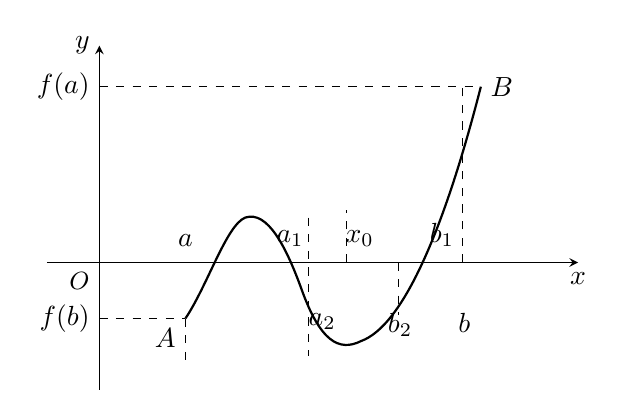
\begin{tikzpicture}[scale=0.95,>=stealth]
  \draw[->] (-0.7,0) -- (6.4,0) node[below] {$x$};
  \draw[->] (0,-1.7) -- (0,2.9) node[left] {$y$};
  \node[below left] at (0,0) {\small $O$};
  \draw[thick] (1.15,-0.75)
    .. controls (1.45,-0.30) and (1.70,0.50) .. (1.95,0.60)
    .. controls (2.25,0.70) and (2.50,0.20) .. (2.70,-0.35)
    .. controls (2.95,-1.05) and (3.20,-1.20) .. (3.50,-1.05)
    .. controls (4.05,-0.85) and (4.60,0.40) .. (5.10,2.35);
  \node[right] at (5.10,2.35) {$B$};
  \node[below left] at (1.15,-0.75) {$A$};
  \draw[dashed] (0,2.35) -- (5.10,2.35);
  \draw[dashed] (0,-0.75) -- (1.15,-0.75);
  \node[left] at (0,2.35) {$f(a)$};
  \node[left] at (0,-0.75) {$f(b)$};
  \draw[dashed] (1.15,-0.75) -- (1.15,-1.30);
  \node[above] at (1.15,0.08) {$a$};
  \draw[dashed] (2.80,0.60) -- (2.80,-1.25);
  \node[above] at (2.55,0.08) {$a_1$};
  \node[below] at (2.98,-0.55) {$a_2$};
  \draw[dashed] (3.30,0) -- (3.30,0.70);
  \node[above] at (3.48,0.08) {$x_0$};
  \draw[dashed] (4.00,0) -- (4.00,-0.70);
  \node[below] at (4.02,-0.55) {$b_2$};
  \draw[dashed] (4.85,0) -- (4.85,2.35);
  \node[above] at (4.58,0.08) {$b_1$};
  \node[below] at (4.88,-0.55) {$b$};
\end{tikzpicture}
\caption{}\label{fig:2.5.1}
\end{figure}

\begin{theoremp}[推广的零(根)值定理]\label{thm:2.5.1p}
设 $f$ 为 $[a,b]$ 上的连续函数, 且 $f(a)f(b) \leqslant 0$, 则 $\exists \xi \in [a,b]$, s.t. $f(\xi) = 0$.
\end{theoremp}

\begin{proof}
如果 $f(a) = 0$, 则取 $\xi = a$; 如果 $f(b) = 0$, 则取 $\xi = b$; 如果 $f(a)f(b) \neq 0$, 则 $f(a)f(b) < 0$, 由零值定理~\ref{thm:2.5.1} 知, $\exists \xi \in (a,b)$, s.t. $f(\xi) = 0$.
\end{proof}

\begin{theorem}[介值定理]\label{thm:2.5.2}
设 $f$ 为 $[a,b]$ 上的连续函数,\allowbreak $f(a) \neq f(b)$,\allowbreak 则 $\forall r \in (\min\{f(a), f(b)\},\allowbreak \max\{f(a), f(b)\})$, $\exists \xi \in (a,b)$, s.t. $f(\xi) = r$.
\end{theorem}

\begin{proof}
令 $F(x) = f(x) - r$, 显然它为 $[a,b]$ 上的连续函数, 且 $F(a)F(b) = (f(a) - r)(f(b) - r) < 0$. 由零值定理~\ref{thm:2.5.1} 知, $\exists \xi \in (a,b)$, s.t. $f(\xi) - r = F(\xi) = 0$, 即 $f(\xi) = r$(如图~\ref{fig:2.5.2} 所示).
\end{proof}

\begin{figure}[htbp]
\centering
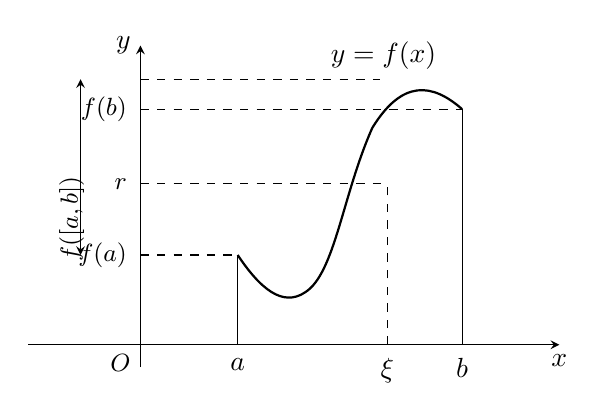
\begin{tikzpicture}[scale=0.95,>=stealth]
  \draw[->] (-1.5,0) -- (5.6,0) node[below] {$x$};
  \draw[->] (0,-0.3) -- (0,4.0) node[left] {$y$};
  \node[below left] at (0,0) {\small $O$};
  \draw[thick] (1.30,1.20)
    .. controls (1.60,0.75) and (1.90,0.50) .. (2.20,0.70)
    .. controls (2.60,0.95) and (2.70,2.00) .. (3.10,2.90)
    .. controls (3.50,3.55) and (3.90,3.50) .. (4.30,3.15);
  \node[above] at (3.25,3.55) {$y=f(x)$};
  \draw (1.30,1.20) -- (1.30,0);
  \draw (4.30,3.15) -- (4.30,0);
  \node[below] at (1.30,-0.05) {$a$};
  \node[below] at (4.30,-0.05) {$b$};
  \draw[dashed] (0,1.20) -- (1.32,1.20);
  \node[left,font=\small] at (-0.05,1.20) {$f(a)$};
  \draw[dashed] (0,3.15) -- (4.30,3.15);
  \node[left,font=\small] at (-0.05,3.15) {$f(b)$};
  \draw[dashed] (0,2.15) -- (3.30,2.15);
  \node[left,font=\small] at (-0.05,2.15) {$r$};
  \draw[dashed] (3.30,0) -- (3.30,2.15);
  \node[below] at (3.30,-0.05) {$\xi$};
  \draw[dashed] (0,3.55) -- (3.20,3.55);
  \draw[<->] (-0.80,1.20) -- (-0.80,3.55);
  \node[left,rotate=90,font=\small] at (-0.92,2.38) {$f([a,b])$};
\end{tikzpicture}
\caption{}\label{fig:2.5.2}
\end{figure}

\begin{theoremp}[推广的介值定理]\label{thm:2.5.2p}
设 $f$ 为 $[a,b]$ 上的连续函数,\allowbreak 则 $\forall r \in [\min\{f(a), f(b)\},\allowbreak \max\{f(a), f(b)\}]$, $\exists \xi \in [a,b]$, s.t. $f(\xi) = r$.
\end{theoremp}

\begin{proof}
不妨设 $f(a) \leqslant f(b)$. 如果 $r = \min\{f(a), f(b)\} = f(a)$, 则取 $\xi = a$; 如果 $r = \max\{f(a), f(b)\} = f(b)$, 则取 $\xi = b$. 如果 $f(a) = \min\{f(a), f(b)\} < r < \max\{f(a), f(b)\} = f(b)$, 则由介值定理~\ref{thm:2.5.2} 知, $\exists \xi \in (a,b)$, s.t. $f(\xi) = r$.

或者将推广的零值定理~\ref{thm:2.5.1p} 用于函数 $F(x) = f(x) - r$ 知, $\exists \xi \in [a,b]$, s.t. $0 = F(\xi) = f(\xi) - r$, 即 $f(\xi) = r$.
\end{proof}

\begin{corollary}\label{cor:2.5.1}
设 $f$ 为区间 $I$(开或半开半闭或闭)上的连续函数, 则 $f$ 的值域 $f(I) = \{f(x) \mid x \in I\}$ 也为一个区间(可退缩为一点).
\end{corollary}

\begin{proof}
若 $f$ 为常值函数, 即 $f(x) \equiv c$(常数), 则 $f(I) = \{c\}$ 退缩为一点.

若 $f$ 不为常值函数, 则必有 $y_1, y_2 \in f(I)$, s.t. $y_1 < y_2$. 由推广的介值定理~\ref{thm:2.5.2p} 知, $\forall r \in [y_1, y_2]$, 必 $\exists \xi \in I$, s.t. $r = f(\xi) \in f(I)$. 所以, $[y_1, y_2] \subset f(I)$. 由 $y_1, y_2$ 的任意性知, $f(I)$ 为一个区间.
\end{proof}

\begin{theorem}[最值定理]\label{thm:2.5.3}
设 $f$ 为有界闭区间 $[a,b]$ 上的连续函数, 则 $f$ 在 $[a,b]$ 上必达到最大值与最小值, 即必存在 $x_*, x^* \in [a,b]$, s.t.
\[
f(x_*) = \min_{x \in [a,b]} f(x) = m,
\]
\[
f(x^*) = \max_{x \in [a,b]} f(x) = M.
\]
\end{theorem}

\begin{proof}
记 $M = \sup\limits_{x \in [a,b]} f(x)$, 则 $M > -\infty$. 任取实数列 $\{\alpha_n\}$, s.t. $\alpha_n < M$ 且 $\{\alpha_n\}$ 严格增趋于 $M$. $\forall n \in \mathbb{N}$, $\alpha_n$ 不是 $f$ 在 $[a,b]$ 上的上界, 故 $\exists x_n \in [a,b]$, s.t. $\alpha_n < f(x_n) \leqslant M$. $\{x_n \mid n \in \mathbb{N}\} \subset [a,b]$ 为有界数列, 根据实数连续性命题(六)(序列紧性)知, 它有收敛子列 $x_{n_k}$. 令 $\lim\limits_{k \to +\infty} x_{n_k} = x^* \in [a,b]$, 由夹逼定理得到 $\lim\limits_{n \to +\infty} f(x_n) = \lim\limits_{n \to +\infty} \alpha_n = M$. 于是, 根据 $f$ 的连续性, 有
\[
M = \lim_{k \to +\infty} f(x_{n_k}) = f(x^*) \leqslant M,
\]
\[
f(x^*) = M,
\]
即 $f(x^*)$ 为 $f$ 在 $[a,b]$ 上的最大值.

同理可证, $\exists x_* \in [a,b]$, s.t. $f(x_*) = m = \inf\limits_{x \in [a,b]} f(x)$, 或用 $-f$ 代 $f$ 再应用上述所得结果.
\end{proof}

由此知, $f$ 在 $[a,b]$ 上为有界函数, 再由介值定理立即得到 $f$ 的值域
\[
f([a,b]) = \left[\min_{x \in [a,b]} f(x), \max_{x \in [a,b]} f(x)\right] = [m, M]
\]
为一个闭区间(包括退缩为一点, 此时 $f$ 为常值函数).

\begin{example}[不动点存在定理, Brouwer]\label{ex:2.5.1}
设 $f$ 在 $[a,b]$ 上连续, 满足 $a \leqslant f(x) \leqslant b, \forall x \in [a,b]$, 即 $f([a,b]) \subset [a,b]$, 则 $\exists \xi \in [a,b]$, s.t. $f(\xi) = \xi$, 称 $\xi$ 为 $f$ 的不动点.
\end{example}

\begin{proof}
令 $F(x) = f(x) - x$, 由 $f$ 连续知, $F$ 连续, 又因 $F(a)F(b) = (f(a) - a)(f(b) - b) \leqslant 0$, 根据推广零值定理~\ref{thm:2.5.1p} 知, $\exists \xi \in [a,b]$, s.t.
\[
f(\xi) - \xi = F(\xi) = 0,
\]
即 $f(\xi) = \xi$(如图~\ref{fig:2.5.3} 所示).
\end{proof}

\begin{figure}[htbp]
\centering
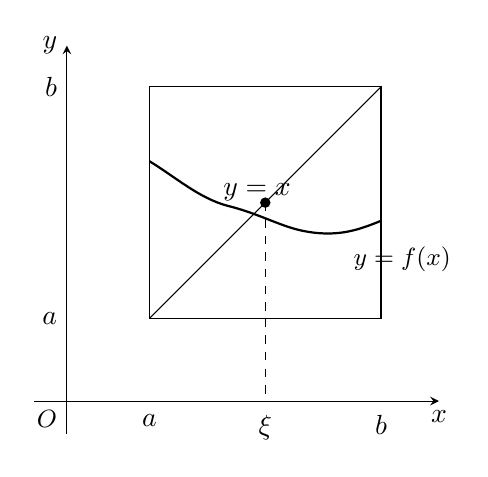
\begin{tikzpicture}[scale=1.05,>=stealth]
  \draw[->] (-0.4,0) -- (4.5,0) node[below] {$x$};
  \draw[->] (0,-0.4) -- (0,4.3) node[left] {$y$};
  \node[below left] at (0,0) {\small $O$};
  \draw (1.00,1.00) rectangle (3.80,3.80);
  \draw (1.00,1.00) -- (3.80,3.80);
  \node[above,sloped] at (2.30,2.30) {$y=x$};
  \draw[thick] (1.00,2.90)
    .. controls (1.30,2.72) and (1.60,2.45) .. (1.95,2.36)
    .. controls (2.35,2.26) and (2.60,2.10) .. (2.90,2.05)
    .. controls (3.30,1.98) and (3.55,2.08) .. (3.80,2.18);
  \node[below right,font=\small] at (3.35,1.98) {$y=f(x)$};
  \fill (2.40,2.40) circle (1.8pt);
  \draw[dashed] (2.40,2.40) -- (2.40,0);
  \node[below] at (1.00,-0.05) {$a$};
  \node[below] at (3.80,-0.05) {$b$};
  \node[below] at (2.40,-0.05) {$\xi$};
  \node[left] at (0,1.00) {$a$};
  \node[left] at (0,3.80) {$b$};
\end{tikzpicture}
\caption{}\label{fig:2.5.3}
\end{figure}

利用零值定理与介值定理可判断代数方程的根的存在范围.

\begin{example}\label{ex:2.5.2}
证明: 方程 $2^x = 4x$ 在 $\left(0, \frac{1}{2}\right)$ 中有根.
\end{example}

\begin{proof}
设 $f(x) = 2^x - 4x$, 它为初等函数, 因而是 $\left[0, \frac{1}{2}\right]$ 上的连续函数, 又 $f(0) = 2^0 - 4 \cdot 0 = 1 > 0$, $f\left(\frac{1}{2}\right) = 2^{\frac{1}{2}} - 4 \cdot \frac{1}{2} = \sqrt{2} - 2 < 0$, 则 $f(0)f\left(\frac{1}{2}\right) < 0$, 由零值定理~\ref{thm:2.5.1} 知, $\exists \xi \in \left(0, \frac{1}{2}\right)$, s.t.
\[
0 = f(\xi) = 2^{\xi} - 4\xi,
\]
即 $2^{\xi} = 4\xi, \xi \in \left(0, \frac{1}{2}\right)$ 为方程 $2^x = 4x$ 的一个根.
\end{proof}

\begin{example}\label{ex:2.5.3}
设 $f$ 在 $[a,b]$ 上连续, $x_1, x_2, \cdots, x_m \in [a,b]$, $\lambda_1, \lambda_2, \cdots, \lambda_m > 0$, $\sum\limits_{i=1}^{m} \lambda_i = 1$, 则 $\exists \xi \in [\min\{x_1, x_2, \cdots, x_m\}, \max\{x_1, x_2, \cdots, x_m\}] \subset [a,b]$, s.t.
\[
f(\xi) = \sum_{i=1}^{m} \lambda_i f(x_i).
\]
特别地, $\exists \xi \in [a,b]$, s.t. $f(\xi) = \frac{f(a) + f(b)}{2}$.
\end{example}

\begin{proof}
因为 $f$ 在 $[a,b]$ 上连续, 且
\[
\min\{f(x_1), f(x_2), \cdots, f(x_m)\} \leqslant \sum_{i=1}^{m} \lambda_i f(x_i) \leqslant \max\{f(x_1), f(x_2), \cdots, f(x_m)\},
\]
所以根据介值定理~\ref{thm:2.5.2} 知, $\exists \xi \in [\min\{x_1, x_2, \cdots, x_m\}, \max\{x_1, x_2, \cdots, x_m\}] \subset [a,b]$, s.t. $f(\xi) = \sum\limits_{i=1}^{m} \lambda_i f(x_i)$. 特别地, 当 $m = 2, x_1 = a, x_2 = b$, $\lambda_1 = \lambda_2 = \frac{1}{2}$ 时, $\exists \xi \in [a,b]$, s.t. $f(\xi) = \frac{f(a) + f(b)}{2}$.
\end{proof}

\begin{example}\label{ex:2.5.4}
证明: 实系数奇次多项式
\[
P(x) = x^{2n+1} + a_1 x^{2n} + \cdots + a_{2n} x + a_{2n+1}
\]
必有实根.
\end{example}

\begin{proof}
因为
\[
\lim_{x \to +\infty} P(x) = \lim_{x \to +\infty} x^{2n+1}\left(1 + \frac{a_1}{x} + \cdots + \frac{a_{2n}}{x^{2n}} + \frac{a_{2n+1}}{x^{2n+1}}\right) = +\infty,
\]
\[
\lim_{x \to -\infty} P(x) = \lim_{x \to -\infty} x^{2n+1}\left(1 + \frac{a_1}{x} + \cdots + \frac{a_{2n}}{x^{2n}} + \frac{a_{2n+1}}{x^{2n+1}}\right) = -\infty,
\]
故 $\exists \Delta > 0$, 当 $x > \Delta$ 时, $P(x) > 1$; 当 $x < -\Delta$ 时, $P(x) < -1$. 取 $a, b$, s.t. $a < -\Delta < \Delta < b$, 则 $P(a) < -1$, $P(b) > 1$. 又因多项式函数 $P(x)$ 为初等函数, 故它为 $\mathbb{R}$ 上的连续函数. 根据零值定理~\ref{thm:2.5.1}, $\exists \xi \in (a,b)$, s.t. $P(\xi) = 0$, 即实系数多项式 $P(x)$ 必有实根.
\end{proof}

\begin{example}\label{ex:2.5.5}
证明: $\tan x = x$ 有无穷个根.
\end{example}

\begin{proof}
设 $f(x) = \tan x - x, x \neq k\pi + \frac{\pi}{2}, k \in \mathbb{Z}$. 显然, 初等函数 $f(x) = \tan x - x$ 在其定义域中为连续函数, 因
\[
\lim_{x \to \left(k\pi + \frac{\pi}{2}\right)^-} (\tan x - x) = +\infty,
\]
\[
\lim_{x \to \left(k\pi - \frac{\pi}{2}\right)^+} (\tan x - x) = -\infty,
\]
故对每个固定的 $k \in \mathbb{Z}$, $\exists a_k, b_k$, s.t.
\[
k\pi - \frac{\pi}{2} < a_k < b_k < k\pi + \frac{\pi}{2},
\]
且 $f(a_k) < 0$, $f(b_k) > 0$. 根据零值定理~\ref{thm:2.5.1} 知, $\exists \xi_k \in (a_k, b_k) \subset \left(k\pi - \frac{\pi}{2}, k\pi + \frac{\pi}{2}\right)$, s.t.
\[
0 = f(\xi_k) = \tan \xi_k - \xi_k,
\]
即 $\tan \xi_k = \xi_k, k \in \mathbb{Z}$. 所以, $\tan x = x$ 有无穷个根(如图~\ref{fig:2.5.4} 所示).
\end{proof}

\begin{figure}[htbp]
\centering
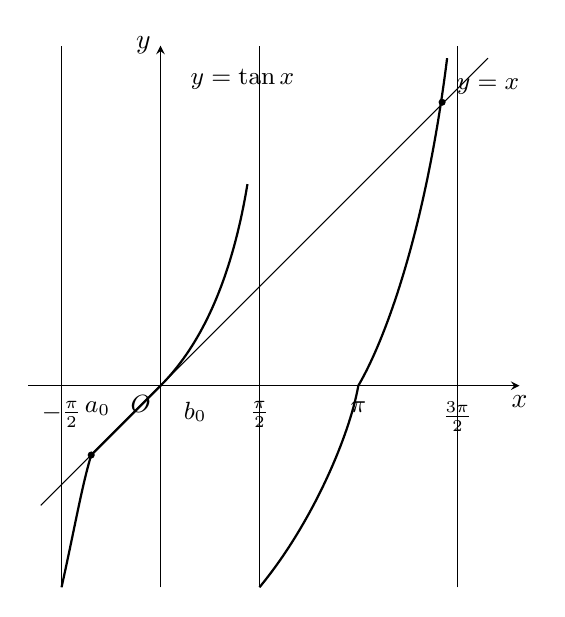
\begin{tikzpicture}[scale=0.80,>=stealth]
  \draw[->] (-2.1,0) -- (5.7,0) node[below] {$x$};
  \draw[->] (0,-3.2) -- (0,5.4) node[left] {$y$};
  \node[below left] at (0,0) {\small $O$};
  \draw (-1.571,-3.2) -- (-1.571,5.4);
  \draw (1.571,-3.2) -- (1.571,5.4);
  \draw (4.712,-3.2) -- (4.712,5.4);
  \draw[thick] (-1.571,-3.2)
     .. controls (-1.35,-2.20) and (-1.25,-1.60) .. (-1.10,-1.10)
     .. controls (-0.60,-0.60) and (-0.30,-0.30) .. (0,0)
     .. controls (0.55,0.55) and (1.10,1.50) .. (1.38,3.20);
  \draw[thick] (1.571,-3.2)
     .. controls (2.40,-2.20) and (3.00,-0.80) .. (3.14,0)
     .. controls (3.55,0.70) and (4.20,2.40) .. (4.55,5.20);
  \draw (-1.9,-1.9) -- (5.2,5.2);
  \node[right,font=\small] at (4.55,4.75) {$y=x$};
  \node[above,font=\small] at (1.30,4.55) {$y=\tan x$};
  \fill (-1.10,-1.10) circle (1.6pt);
  \fill (4.47,4.50) circle (1.6pt);
  \node[below,font=\small] at (-1.571,-0.10) {$-\frac{\pi}{2}$};
  \node[below,font=\small] at (-1.00,-0.10) {$a_0$};
  \node[below,font=\small] at (0.55,-0.10) {$b_0$};
  \node[below,font=\small] at (1.571,-0.10) {$\frac{\pi}{2}$};
  \node[below,font=\small] at (3.14,-0.10) {$\pi$};
  \node[below,font=\small] at (4.712,-0.10) {$\frac{3\pi}{2}$};
\end{tikzpicture}
\caption{}\label{fig:2.5.4}
\end{figure}

\begin{example}\label{ex:2.5.6}
设函数 $f$ 在 $(a,b)$ 上连续, 且 $f(a^+), f(b^-)$ 存在有限, 则 $f$ 在 $(a,b)$ 上有界.
\end{example}

\begin{proof}
\textbf{证法 1}\quad 令
\[
\tilde{f}(x) = \begin{cases} f(x), & x \in (a,b), \\ f(a^+), & x = a, \\ f(b^-), & x = b. \end{cases}
\]
显然, $\tilde{f}$ 在 $[a,b]$ 上连续, 根据最值定理~\ref{thm:2.5.3} 知, $\exists x_*, x^* \in [a,b]$, s.t. $\tilde{f}(x_*) = \min\limits_{x \in [a,b]} \tilde{f}(x) \leqslant f(x) \leqslant \max\limits_{x \in [a,b]} \tilde{f}(x) = \tilde{f}(x^*)$, $\forall x \in (a,b)$, 从而, $f$ 在 $(a,b)$ 上有界.

\textbf{证法 2}\quad 因 $f(a^+), f(b^-)$ 存在有限, 所以, 对 $\varepsilon_0 = 1$, $\exists \delta > 0$, s.t. $a < a + \delta < b - \delta < b$, 且
\[
f(a^+) - 1 < f(x) < f(a^+) + 1, \quad a < x < a + \delta,
\]
\[
f(b^-) - 1 < f(x) < f(b^-) + 1, \quad b - \delta < x < b.
\]
由 $f$ 在 $[a+\delta, b-\delta]$ 上连续, 并根据最值定理~\ref{thm:2.5.3} 知,
\[
|f(x)| \leqslant L, \forall x \in [a+\delta, b-\delta].
\]
所以, $|f(x)| \leqslant M = \max\{L, |f(a^+) - 1|, |f(a^+) + 1|, |f(b^-) - 1|, |f(b^-) + 1|\}$, 即 $f$ 在 $(a,b)$ 上有界.
\end{proof}

\begin{example}\label{ex:2.5.7}
设 $f$ 在 $(-\infty, +\infty)$ 上连续, 且 $\lim\limits_{x \to \infty} f(x)$ 存在有限, 则 $f$ 在 $(-\infty, +\infty)$ 上有界, 且 $f$ 在 $(-\infty, +\infty)$ 上必达到最大值或最小值.
\end{example}

\begin{proof}
设 $\lim\limits_{x \to \infty} f(x) = a \in \mathbb{R}$.

如果 $f(x) \equiv a, \forall x \in (-\infty, +\infty)$, 则 $f$ 在 $(-\infty, +\infty)$ 上有界, 且 $f$ 在其上达到最大值或最小值 $a$.

如果 $f(x) \not\equiv a$, 则 $\exists x_0 \in (-\infty, +\infty)$, s.t. $f(x_0) \neq a$.

若 $f(x_0) < a$, 取 $\varepsilon_0 \in (0, a - f(x_0))$, 因为 $\lim\limits_{x \to \infty} f(x) = a$, 故 $\exists \Delta > 0$, 当 $|x| > \Delta$ 时, 有 $f(x) > a - \varepsilon_0 > a - (a - f(x_0)) = f(x_0)$. 又因 $f$ 连续, 并根据最值定理~\ref{thm:2.5.3} 知, $\exists x_* \in [-\Delta, \Delta]$, s.t.
\[
f(x_*) = \min_{x \in [-\Delta, \Delta]} f(x) \leqslant f(x_0).
\]
于是(如图~\ref{fig:2.5.5} 所示),
\[
f(x_*) = \min_{x \in (-\infty, +\infty)} f(x).
\]
若 $f(x_0) > a$, 类似上述证明或用 $-f$ 代 $f$ 得 $x^* \in (-\infty, +\infty)$, s.t.
\[
f(x^*) = \max_{x \in (-\infty, +\infty)} f(x).
\]
\end{proof}

\begin{figure}[htbp]
\centering
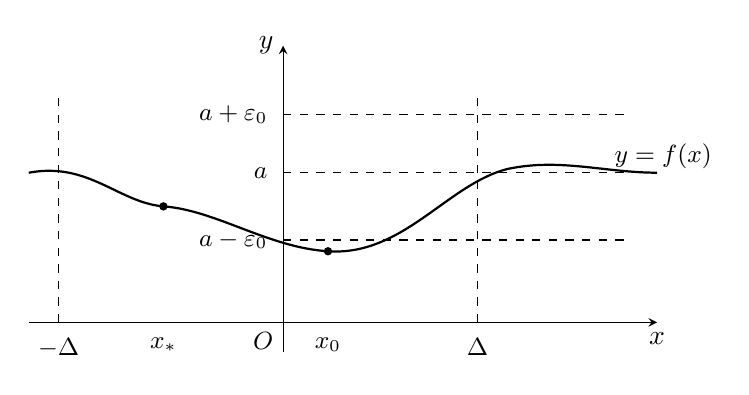
\begin{tikzpicture}[scale=0.95,>=stealth]
  \draw[->] (-3.4,0) -- (5.0,0) node[below] {$x$};
  \draw[->] (0,-0.4) -- (0,3.7) node[left] {$y$};
  \node[below left] at (0,0) {\small $O$};
  \draw[thick] (-3.4,2.00)
     .. controls (-2.60,2.15) and (-2.20,1.60) .. (-1.60,1.55)
     .. controls (-0.90,1.50) and (-0.20,1.00) .. (0.60,0.95)
     .. controls (1.60,0.88) and (2.20,1.85) .. (3.00,2.05)
     .. controls (3.70,2.20) and (4.30,2.00) .. (5.0,2.00);
  \node[right,font=\small] at (4.30,2.22) {$y=f(x)$};
  \draw[dashed] (0,2.00) -- (5.0,2.00);
  \draw[dashed] (0,2.78) -- (4.60,2.78);
  \draw[dashed] (0,1.10) -- (4.60,1.10);
  \node[left,font=\small] at (-0.08,2.00) {$a$};
  \node[left,font=\small] at (-0.08,2.78) {$a+\varepsilon_0$};
  \node[left,font=\small] at (-0.08,1.10) {$a-\varepsilon_0$};
  \draw[dashed] (-3.00,0) -- (-3.00,3.10);
  \draw[dashed] (2.60,0) -- (2.60,3.10);
  \node[below,font=\small] at (-3.00,-0.08) {$-\Delta$};
  \node[below,font=\small] at (2.60,-0.08) {$\Delta$};
  \fill (-1.60,1.55) circle (1.6pt);
  \node[below,font=\small] at (-1.60,-0.08) {$x_*$};
  \fill (0.60,0.95) circle (1.6pt);
  \node[below,font=\small] at (0.60,-0.08) {$x_0$};
\end{tikzpicture}
\caption{}\label{fig:2.5.5}
\end{figure}

为了讨论有界闭区间 $[a,b]$ 上另一个重要的一致连续性定理, 我们先引进一致连续的概念.

\begin{definition}\label{def:2.5.1}
设 $X \subsetneq \mathbb{R}$, $f\colon X \to \mathbb{R}$ 为一元函数. 如果 $\forall \varepsilon > 0$, $\exists \delta = \delta(\varepsilon) > 0$($\delta(\varepsilon)$ 只与 $\varepsilon$ 有关, 而与 $X$ 中的点 $x$ 无关!), 当 $x', x'' \in X$, 且 $x'$ 与 $x''$ 之间的距离 $\rho(x', x'') = |x' - x''|$ 小于 $\delta$, 就有 $|f(x') - f(x'')| < \varepsilon$, 则称 $f$ 在 $X$ 上是\textbf{一致连续}(或\textbf{均匀连续})的.
\end{definition}

\begin{theorem}\label{thm:2.5.4}
如果 $f$ 在 $X$ 上一致连续, 则 $f$ 在 $X$ 上连续. 但反之不真.
\end{theorem}

\begin{proof}
$\forall \varepsilon > 0$, 因 $f$ 在 $X$ 上一致连续, 故 $\exists \delta = \delta(\varepsilon) > 0$, 当 $x', x'' \in X, |x' - x''| < \delta$ 时, 有 $|f(x') - f(x'')| < \varepsilon$. 对 $x_0 \in X$, 当 $x \in X, |x - x_0| < \delta$ 时, 当然有 $|f(x) - f(x_0)| < \varepsilon$, 这就证明了 $f$ 在 $\forall x_0 \in X$ 处是连续的, 即 $f$ 在 $X$ 上连续.
\end{proof}

反之不真有反例: $f(x) = \frac{1}{x}$. 显然, 基本初等函数 $\frac{1}{x} = x^{-1}$ 在 $(0,1)$ 上连续. 但是, 它在 $(0,1)$ 上不一致连续.

\textbf{证法 1}\quad (反证) 假设 $f(x) = \frac{1}{x}$ 在 $(0,1)$ 上一致连续, 对 $\forall \varepsilon > 0, \exists \delta = \delta(\varepsilon) > 0$, 当 $x', x'' \in (0,1), |x' - x''| < \delta$ 时, 有
\[
\left|\frac{1}{x'} - \frac{1}{x''}\right| = |f(x') - f(x'')| < \varepsilon.
\]
取定 $x'' \in (0, \delta)$, 令 $x' \to 0^+$, 得到 $+\infty \leqslant \varepsilon$, 矛盾.

\textbf{证法 2}\quad 取 $\varepsilon_0 = 1, \forall \delta \in \left(0, \frac{1}{2}\right)$, 当 $x' = \frac{\delta}{2}, x'' = \delta$ 时, 虽然 $|x' - x''| = \left|\frac{\delta}{2} - \delta\right| = \frac{\delta}{2} < \delta$, 但
\[
\left|\frac{1}{x'} - \frac{1}{x''}\right| = \left|\frac{1}{\frac{\delta}{2}} - \frac{1}{\delta}\right| = \frac{1}{\delta} > 2 > 1 = \varepsilon_0.
\]
所以, $f(x) = \frac{1}{x}$ 在 $(0,1)$ 上不一致连续.

\textbf{证法 3}\quad 取 $x_n' = \frac{1}{n}, x_n'' = \frac{1}{n+1}$, 虽然
\[
|x_n' - x_n''| = \left|\frac{1}{n} - \frac{1}{n+1}\right| = \frac{1}{n(n+1)} \to 0 \quad (n \to +\infty),
\]
但
\[
|f(x_n') - f(x_n'')| = \left|\frac{1}{\frac{1}{n}} - \frac{1}{\frac{1}{n+1}}\right| = |n - (n+1)| = 1 \not\to 0 \quad (n \to +\infty).
\]
根据下面的定理~\ref{thm:2.5.8} 知, $f(x) = \frac{1}{x}$ 在 $(0,1)$ 上不一致连续.

\begin{theorem}[Cantor 定理]\label{thm:2.5.5}
有界闭区间 $[a,b]$ 上的连续函数是一致连续的.
\end{theorem}

\begin{proof}
\textbf{证法 1}\quad (反证) 假设 $f$ 在 $[a,b]$ 上不一致连续, 根据其定义知, $\exists \varepsilon_0 > 0, \forall n \in \mathbb{N}$, $\exists x_n', x_n'' \in [a,b]$, 虽然 $|x_n' - x_n''| < \frac{1}{n}$, 但
\[
|f(x_n') - f(x_n'')| \geqslant \varepsilon_0.
\]
由于数列 $\{x_n'\}$ 有界, 根据实数连续性命题(六)(序列紧性)知, 存在收敛子列 $\{x_{n_k}'\}$, 记
\[
\lim_{k \to +\infty} x_{n_k}' = x_0 \in [a,b].
\]
另一方面, 由于 $|x_{n_k}' - x_{n_k}''| < \frac{1}{n_k} \leqslant \frac{1}{k} \to 0\ (k \to +\infty)$, 故有 $\lim\limits_{k \to +\infty} x_{n_k}'' = x_0$, 但由上式知, $|f(x_{n_k}') - f(x_{n_k}'')| \geqslant \varepsilon_0$. 所以, 由 $f$ 连续得到
\[
0 = |f(x_0) - f(x_0)| = \lim_{k \to +\infty} |f(x_{n_k}') - f(x_{n_k}'')| \geqslant \varepsilon_0 > 0,
\]
矛盾.

\textbf{证法 2}\quad 因 $f$ 在 $[a,b]$ 上连续, 故 $\forall \varepsilon > 0, \forall x \in [a,b], \exists \delta_x > 0$, s.t. 当 $u \in [a,b] \cap (x - \delta_x, x + \delta_x)$ 时, $|f(u) - f(x)| < \frac{\varepsilon}{2}$. 当 $x', x'' \in [a,b] \cap (x - \delta_x, x + \delta_x)$ 时,
\[
\begin{aligned}
|f(x') - f(x'')| &\leqslant |f(x') - f(x)| + |f(x'') - f(x)| \\
&< \frac{\varepsilon}{2} + \frac{\varepsilon}{2} = \varepsilon.
\end{aligned}
\tag*{(*)}
\]
显然, $\mathcal{I} = \left\{\left(x - \frac{\delta_x}{2}, x + \frac{\delta_x}{2}\right) \mid x \in [a,b]\right\}$ 为 $[a,b]$ 的一个开区间覆盖. 由实数连续性命题(四)($[a,b]$ 的紧致性)知, 存在有限子覆盖 $\mathcal{I}_1 = \left\{\left(x_k - \frac{\delta_{x_k}}{2}, x_k + \frac{\delta_{x_k}}{2}\right) \mid k = 1, 2, \cdots, n\right\} \subset \mathcal{I}$. 令
\[
\delta = \delta(\varepsilon) = \min\left\{\frac{\delta_{x_k}}{2} \mid k = 1, 2, \cdots, n\right\} > 0,
\]
则 $\forall x', x'' \in [a,b], |x' - x''| < \delta$, $\exists k \in \mathbb{N}, 1 \leqslant k \leqslant n$, s.t.
\[
x' \in \left(x_k - \frac{\delta_{x_k}}{2}, x_k + \frac{\delta_{x_k}}{2}\right).
\]
于是,
\[
|x'' - x_k| \leqslant |x'' - x'| + |x' - x_k| < \delta + \frac{\delta_{x_k}}{2} \leqslant \delta_{x_k},
\]
即 $x'' \in (x_k - \delta_{x_k}, x_k + \delta_{x_k})$, 由 $(*)$ 式推得
\[
|f(x') - f(x'')| < \varepsilon,
\]
从而 $f$ 在 $[a,b]$ 上一致连续.

\textbf{证法 3}\quad 在证法 2 中, 令
\[
\tilde{\mathcal{I}} = \{(x - \delta_x, x + \delta_x) \mid x \in [a,b]\},
\]
则 $\tilde{\mathcal{I}}$ 为 $[a,b]$ 的开区间覆盖. 根据下面的 Lebesgue 数定理~\ref{thm:2.5.6} 知, 存在 Lebesgue 数 $\lambda = \lambda(\mathcal{I}) > 0$. $\forall \varepsilon > 0$, 取 $\delta = \delta(\varepsilon) = \lambda(\tilde{\mathcal{I}})$, 则当 $x', x'' \in [a,b]$ 且两点集 $\{x', x''\}$ 的直径为
\[
d(\{x', x''\}) = |x' - x''| < \delta = \lambda(\tilde{\mathcal{I}})
\]
时, 必有 $(x_0 - \delta_{x_0}, x_0 + \delta_{x_0}) \in \tilde{\mathcal{I}}$, s.t. $\{x', x''\} \subset (x_0 - \delta_{x_0}, x_0 + \delta_{x_0})$, 从而,
\[
|f(x') - f(x'')| < \varepsilon.
\]
这就证明了 $f$ 在 $[a,b]$ 上是一致连续的.
\end{proof}

\begin{theorem}[Lebesgue 数定理]\label{thm:2.5.6}
设 $\mathcal{I}$ 为有界闭区间 $[a,b]$ 上的一个开覆盖, 则必存在数 $\lambda = \lambda(\mathcal{I}) > 0$, 使当集合 $A \subset [a,b]$, 其直径 $d(A) = \sup\{\rho(x', x'') \mid x', x'' \in A\} < \lambda = \lambda(\mathcal{I})$ 时, 必有 $I \in \mathcal{I}$, s.t. $A \subset I$. 我们称 $\lambda = \lambda(\mathcal{I})$ 为 $\mathcal{I}$ 的一个 Lebesgue 数.
\end{theorem}

\begin{proof}
(反证) 假设结论不成立, 则 $\forall n \in \mathbb{N}$, 存在 $A_n \subset [a,b]$, 它的直径 $d(A_n) < \frac{1}{n}$, 而不存在 $I \in \mathcal{I}$, s.t. $A_n \subset I$. 在每个 $A_n$ 中取 $a_n$, 根据实数连续性命题(六)(序列紧性)可知, 存在子列 $\{a_{n_k}\}$ 收敛于 $a_0 \in [a,b]$. 因为 $\mathcal{I}$ 为 $[a,b]$ 的开覆盖, 故存在 $I_0 \in \mathcal{I}$, 使得 $a_0 \in I_0$. 因为 $I_0$ 为开集, 当 $[a,b] \setminus I_0 \neq \varnothing$ 时, 点 $a_0$ 到 $[a,b] \setminus I_0$ 的距离
\[
d = \rho(a_0, [a,b] \setminus I_0) = \inf\{\rho(a_0, x) \mid x \in [a,b] \setminus I_0\} > 0.
\]
由于 $\lim\limits_{k \to +\infty} a_{n_k} = a_0$, 所以, $\exists n_{k_0}$, s.t. $n_{k_0} > \frac{2}{d}$ 与 $\rho(a_0, a_{n_{k_0}}) < \frac{d}{2}$. 于是, $\forall x \in A_{n_{k_0}}$, 有
\[
\rho(a_0, x) \leqslant \rho(a_0, a_{n_{k_0}}) + \rho(a_{n_{k_0}}, x) < \frac{d}{2} + \frac{1}{n_{k_0}} < \frac{d}{2} + \frac{d}{2} = d,
\]
因而, $A_{n_{k_0}} \subset I_0 \in \mathcal{I}$; 当 $[a,b] \setminus I_0 = \varnothing$ 时, $A_n \subset [a,b] \subset I_0$, 这与不存在 $I \in \mathcal{I}$ 使得 $A_{n_{k_0}} \subset I$ 相矛盾.
\end{proof}

\begin{theorem}\label{thm:2.5.7}
$f$ 在 $(a,b)$ 上一致连续 $\iff f$ 可延拓为 $[a,b]$ 上的连续函数 $\tilde{f}$, 此时 $\tilde{f}|_{(a,b)} = f|_{(a,b)}$.
\end{theorem}

\begin{proof}
($\Leftarrow$) 设 $f$ 可延拓为 $[a,b]$ 上的连续函数 $\tilde{f}$, 由 Cantor 定理~\ref{thm:2.5.5} 知, $\tilde{f}$ 在 $[a,b]$ 上一致连续, 而 $\tilde{f}|_{(a,b)} = f|_{(a,b)}$, 因此 $f$ 在 $(a,b)$ 上一致连续.

($\Rightarrow$) 设 $f$ 在 $(a,b)$ 上一致连续. $\forall \varepsilon > 0$, $\exists \delta = \delta(\varepsilon) > 0$, 当 $x', x'' \in (a,b), |x' - x''| < \delta$ 时, $|f(x') - f(x'')| < \varepsilon$.

任取 $x_n \in (a,b)$, $x_n \to a^+$, 则 $\{x_n\}$ 为 Cauchy(基本)数列. 因此, $\exists N \in \mathbb{N}$, 当 $m, n > N$ 时, $|x_n - x_m| < \delta$, 从而有 $|f(x_n) - f(x_m)| < \varepsilon$. 这就证明了 $\{f(x_n)\}$ 为 Cauchy(基本)数列. 根据实数连续性命题(七)($\mathbb{R}$ 的完备性)知, $\{f(x_n)\}$ 收敛. $\forall x_n', x_n'' \to a^+\ (n \to +\infty)$, 显然有
\[
\{x_n'''\} \colon x_1', x_1'', x_2', x_2'', \cdots, x_n', x_n'', \cdots \to a^+.
\]
由上证得 $\{f(x_n''')\}$ 收敛, 并且
\[
\lim_{n \to +\infty} f(x_n') = \lim_{n \to +\infty} f(x_n'') = \lim_{n \to +\infty} f(x_n''').
\]
这就证明了 $\forall x_n \to a^+$, $\{f(x_n)\}$ 收敛于同一数, 故 $\lim\limits_{x \to a^+} f(x)$ 存在有限. 同理可证 $\lim\limits_{x \to b^-} f(x)$ 存在有限. 令
\[
\tilde{f}(x) = \begin{cases} f(a^+), & x = a, \\ f(x), & a < x < b, \\ f(b^-), & x = b. \end{cases}
\]
显然, $\tilde{f}$ 为 $[a,b]$ 上的连续函数, 且为 $f$ 的延拓.
\end{proof}

\begin{theorem}\label{thm:2.5.8}
设 $X \subsetneq \mathbb{R}$, $f\colon X \to \mathbb{R}$ 为一元函数. 如果 $\exists x_n', x_n'' \in X, n \in \mathbb{N}$, $|x_n' - x_n''| \to 0$ 但 $|f(x_n') - f(x_n'')| \not\to 0\ (n \to +\infty)$, 则 $f$ 在 $X$ 上不一致连续.
\end{theorem}

\begin{proof}
(反证) 假设 $f$ 在 $X$ 上一致连续, 则 $\forall \varepsilon > 0, \exists \delta = \delta(\varepsilon) > 0$, 当 $x', x'' \in X, |x' - x''| < \delta$ 时, $|f(x') - f(x'')| < \varepsilon$. 因 $|x_n' - x_n''| \to 0\ (n \to +\infty)$, 故 $\exists N \in \mathbb{N}$, 当 $n > N$ 时, $|x_n' - x_n''| < \delta$, 从而有
\[
|f(x_n') - f(x_n'')| < \varepsilon.
\]
由此就推得 $|f(x_n') - f(x_n'')| \to 0\ (n \to +\infty)$, 这与题设 $|f(x_n') - f(x_n'')| \not\to 0\ (n \to +\infty)$ 相矛盾.
\end{proof}

\begin{example}\label{ex:2.5.8}
设 $X \subsetneq \mathbb{R}$, $f\colon X \to \mathbb{R}$ 为一元函数, 它满足 Lipschitz 条件, 即 $\forall x', x'' \in X$, 有 $|f(x') - f(x'')| \leqslant M|x' - x''|$, 其中 $M$ 为常数, 则 $f$ 在 $X$ 上为一致连续函数.
\end{example}

\begin{proof}
$\forall \varepsilon > 0$, 取 $\delta \in \left(0, \frac{\varepsilon}{M+1}\right)$, 当 $x', x'' \in X$, 且 $|x' - x''| < \delta$ 时,
\[
|f(x') - f(x'')| \leqslant M|x' - x''| \leqslant M\delta < M \cdot \frac{\varepsilon}{M+1} < \varepsilon.
\]
因此, $f$ 在 $X$ 上为一致连续函数.
\end{proof}

\begin{example}\label{ex:2.5.9}
(1) $f(x) = \frac{1}{x}$ 在 $[a,b]$ 上一致连续, $0 < a < b$;

(2) $f(x) = ax + b$ 在 $(-\infty, +\infty)$ 内一致连续;

(3) $f(x) = x^2$ 在 $(-\infty, +\infty)$ 内不一致连续;

(4) $f(x) = \sin x^2$ 在 $(-\infty, +\infty)$ 内不一致连续;

(5) $f(x) = \sin \frac{1}{x}$ 在 $(0,1)$ 上不一致连续.
\end{example}

\begin{proof}
(1) $\forall \varepsilon > 0$, 取 $\delta \in (0, a^2\varepsilon)$, 当 $x', x'' \in [a,b], |x' - x''| < \delta$ 时,
\[
\left|\frac{1}{x'} - \frac{1}{x''}\right| = \frac{|x' - x''|}{x'x''} \leqslant \frac{|x' - x''|}{a^2} < \frac{\delta}{a^2} < \varepsilon,
\]
所以, $f(x) = \frac{1}{x}$ 在 $[a,b]$ 上一致连续.

(2) $\forall \varepsilon > 0$, 取 $\delta \in \left(0, \frac{\varepsilon}{|a|+1}\right)$, 当 $x', x'' \in (-\infty, +\infty), |x' - x''| < \delta$ 时,
\[
\begin{aligned}
|f(x') - f(x'')| &= |(ax' + b) - (ax'' + b)| = |ax' - ax''| \\
&= |a| \cdot |x' - x''| \leqslant (|a| + 1)\delta < \varepsilon,
\end{aligned}
\]
所以, $f(x) = ax + b$ 在 $(-\infty, +\infty)$ 内一致连续.

(3) 取 $x_n' = n, x_n'' = n + \frac{1}{n}$, 则 $|x_n' - x_n''| = \left|n - \left(n + \frac{1}{n}\right)\right| = \frac{1}{n} \to 0\ (n \to +\infty)$, 而
\[
|f(x_n') - f(x_n'')| = \left|n^2 - \left(n + \frac{1}{n}\right)^2\right| = 2 + \frac{1}{n^2} \to 2 \neq 0 \quad (n \to +\infty).
\]
根据定理~\ref{thm:2.5.8} 知, $f(x) = x^2$ 在 $(-\infty, +\infty)$ 内不一致连续.

(4) 取 $x_n' = \sqrt{2n\pi + \frac{\pi}{2}}, x_n'' = \sqrt{2n\pi}$, 则
\[
\begin{aligned}
|x_n' - x_n''| &= \left|\sqrt{2n\pi + \frac{\pi}{2}} - \sqrt{2n\pi}\right| \\
&= \frac{\frac{\pi}{2}}{\sqrt{2n\pi + \frac{\pi}{2}} + \sqrt{2n\pi}} \to 0 \quad (n \to +\infty),
\end{aligned}
\]
但
\[
\begin{aligned}
|f(x_n') - f(x_n'')| &= |\sin(x_n')^2 - \sin(x_n'')^2| \\
&= \left|\sin\left(2n\pi + \frac{\pi}{2}\right) - \sin 2n\pi\right| \\
&= |1 - 0| = 1 \not\to 0 \quad (n \to +\infty),
\end{aligned}
\]
根据定理~\ref{thm:2.5.8} 知, $f(x) = \sin x^2$ 在 $(-\infty, +\infty)$ 内不一致连续.

(5) \textbf{证法 1}\quad 取 $x_n' = \frac{1}{2n\pi}, x_n'' = \frac{1}{2n\pi + \frac{\pi}{2}}$, 则
\[
|x_n' - x_n''| = \left|\frac{1}{2n\pi} - \frac{1}{2n\pi + \frac{\pi}{2}}\right| = \frac{\frac{\pi}{2}}{2n\pi\left(2n\pi + \frac{\pi}{2}\right)} \to 0 \quad (n \to +\infty),
\]
但
\[
\begin{aligned}
|f(x_n') - f(x_n'')| &= \left|\sin\frac{1}{x_n'} - \sin\frac{1}{x_n''}\right| = \left|\sin 2n\pi - \sin\left(2n\pi + \frac{\pi}{2}\right)\right| \\
&= |0 - 1| = 1 \not\to 0 \quad (n \to +\infty),
\end{aligned}
\]
根据定理~\ref{thm:2.5.8} 知, $f(x) = \sin\frac{1}{x}$ 在 $(0,1)$ 上不一致连续.

\textbf{证法 2}\quad (反证) 假设 $f(x) = \sin\frac{1}{x}$ 在 $(0,1)$ 上一致连续, 由定理~\ref{thm:2.5.7} 知, $f(x)$ 可延拓为 $[0,1]$ 上的连续函数 $\tilde{f}(x)$, 因而 $\tilde{f}(0) = \lim\limits_{x \to 0^+} \tilde{f}(x) = \lim\limits_{x \to 0^+} \sin\frac{1}{x}$ 存在有限, 这与 $\lim\limits_{x \to 0^+} \sin\frac{1}{x}$ 显然不存在相矛盾.
\end{proof}

\begin{example}\label{ex:2.5.10}
设 $f$ 在 $[a,+\infty)$ 上连续, 且 $\lim\limits_{x \to +\infty} f(x)$ 存在有限, 则 $f$ 在 $[a,+\infty)$ 上一致连续.
\end{example}

\begin{proof}
\textbf{证法 1}\quad 因 $\lim\limits_{x \to +\infty} f(x) = A \in \mathbb{R}$, 故 $\forall \varepsilon > 0$, 必 $\exists \Delta > 0$, 当 $x > \Delta$ 时, 有 $|f(x) - A| < \frac{\varepsilon}{2}$.

又因 $f$ 连续, 根据 Cantor 定理~\ref{thm:2.5.5} 知, $f$ 在 $[a,\Delta]$ 上一致连续, 故 $\exists \delta_1 > 0$, 当 $x', x'' \in [a,\Delta], |x' - x''| < \delta_1$ 时, 有
\[
|f(x') - f(x'')| < \varepsilon.
\]
由于 $f$ 在点 $\Delta$ 处连续, 所以 $\exists \delta_2 > 0$, 当 $|x - \Delta| < \delta_2$ 时, 有
\[
|f(x) - f(\Delta)| < \frac{\varepsilon}{2}.
\]
令 $\delta = \min\{\delta_1, \delta_2\} > 0$, 当 $x', x'' \in [a,+\infty), |x' - x''| < \delta$ 时, 必有下面结论:

(1) $x', x'' \in (\Delta, +\infty)$, 则
\[
|f(x') - f(x'')| \leqslant |f(x') - A| + |f(x'') - A| < \frac{\varepsilon}{2} + \frac{\varepsilon}{2} = \varepsilon.
\]

(2) $x', x'' \in [a,\Delta]$, 则 $|f(x') - f(x'')| < \varepsilon$.

(3) $x' \in [a,\Delta], x'' \in [\Delta,+\infty)$, 则
\[
|x' - \Delta| < x'' - x' < \delta \leqslant \delta_2,
\]
\[
|f(x') - f(\Delta)| < \frac{\varepsilon}{2}.
\]
同理, $|f(x'') - f(\Delta)| < \frac{\varepsilon}{2}$. 因此,
\[
|f(x') - f(x'')| \leqslant |f(x') - f(\Delta)| + |f(x'') - f(\Delta)| < \frac{\varepsilon}{2} + \frac{\varepsilon}{2} = \varepsilon.
\]
这就证明了 $f$ 在 $[a,+\infty)$ 上是一致连续的.

\textbf{证法 2}\quad 因 $\lim\limits_{x \to +\infty} f(x) = A \in \mathbb{R}$, 故 $\forall \varepsilon > 0$, 必 $\exists \Delta > 0$, 当 $x > \Delta$ 时, 有 $|f(x) - A| < \frac{\varepsilon}{2}$.

又因 $f$ 连续, 根据 Cantor 定理~\ref{thm:2.5.5} 知, $f$ 在 $[a,\Delta+1]$ 上一致连续, 故 $\exists \delta_1 > 0$, 当 $x', x'' \in [a,\Delta+1], |x' - x''| < \delta_1$ 时, 有
\[
|f(x') - f(x'')| < \varepsilon.
\]
令 $\delta = \min\{1, \delta_1\}$, 当 $x', x'' \in [a,+\infty), x' < x'', |x' - x''| < \delta$ 时, 必有下面结论:

(1) $x', x'' \in (\Delta, +\infty)$, 则
\[
|f(x') - f(x'')| \leqslant |f(x') - A| + |f(x'') - A| < \frac{\varepsilon}{2} + \frac{\varepsilon}{2} = \varepsilon.
\]

(2) $x', x'' \in [a, \Delta+1]$, 则
\[
|f(x') - f(x'')| < \varepsilon.
\]

(3) 若 $a \leqslant x' < \Delta < \Delta + 1 < x''$, 则
\[
1 = (\Delta + 1) - \Delta < |x' - x''| < \delta \leqslant 1,
\]
矛盾. 由此推得这种情形不出现.

综合上述知, $f$ 在 $[a,+\infty)$ 上一致连续.
\end{proof}

\begin{example}\label{ex:2.5.11}
设 $f\colon (-\infty, +\infty) \to \mathbb{R}$ 是以 $T > 0$ 为周期的连续函数, 则 $f$ 在 $(-\infty, +\infty)$ 上一致连续.
\end{example}

\begin{proof}
\textbf{证法 1}\quad 因 $f$ 是以 $T > 0$ 为周期的函数, 根据 Cantor 定理~\ref{thm:2.5.5} 知, $\forall \varepsilon > 0, \exists \delta_1 > 0$, 当 $x', x'' \in [kT, (k+1)T], k \in \mathbb{Z}$ 时,
\[
|f(x') - f(x'')| < \varepsilon.
\]
$\forall kT, \exists \delta_2 > 0$, 当 $|x - kT| < \delta_2$ 时, 有
\[
|f(x) - f(kT)| < \frac{\varepsilon}{2}.
\]
于是, $\forall x', x'' \in (kT - \delta_2, kT + \delta_2)$,
\[
|f(x') - f(x'')| \leqslant |f(x') - f(kT)| + |f(x'') - f(kT)| < \frac{\varepsilon}{2} + \frac{\varepsilon}{2} = \varepsilon.
\]
令 $\delta = \min\{T, \delta_1, \delta_2\}$, 则当 $x', x'' \in (-\infty, +\infty)$, $x' \leqslant x''$, $|x' - x''| < \delta$ 时, 有下面结论:

(1) $x', x'' \in [kT, (k+1)T]$, 则 $|f(x') - f(x'')| < \varepsilon$;

(2) $x' \in [(k-1)T, kT], x'' \in [kT, (k+1)T]$, 则
\[
|x' - kT| \leqslant |x' - x''| < \delta \leqslant \delta_2,
\]
\[
|x'' - kT| \leqslant |x' - x''| < \delta \leqslant \delta_2,
\]
\[
|f(x') - f(x'')| < \varepsilon.
\]
这就证明了 $f$ 在 $(-\infty, +\infty)$ 上是一致连续的.

\textbf{证法 2}\quad 因 $f$ 在 $[0,2T]$ 内连续, 根据 Cantor 定理~\ref{thm:2.5.5} 知, $f$ 在 $[0,2T]$ 内一致连续, 故 $\forall \varepsilon > 0$, 取 $\delta_1 > 0$, 当 $x', x'' \in [0,2T], |x' - x''| < \delta_1$ 时, 有 $|f(x') - f(x'')| < \varepsilon$.

令 $\delta = \min\{T, \delta_1\}$, 当 $x', x'' \in (-\infty, +\infty)$, $x' < x''$, 且 $|x' - x''| < \delta$ 时, 必有 $n \in \mathbb{Z}$, s.t. $x' = nT + x_0'$, 其中 $x_0' \in [0, T]$, 则 $x'' = nT + x_0''$, $x_0'' \in [0, 2T]$. 于是, $|x_0' - x_0''| = |(x' - nT) - (x'' - nT)| = |x' - x''| < \delta$,
\[
|f(x') - f(x'')| = |f(x_0') - f(x_0'')| < \varepsilon.
\]
这就证明了 $f$ 在 $(-\infty, +\infty)$ 内一致连续.
\end{proof}

\begin{exblock}{练习题 2.5}
\item 用 $\varepsilon$-$\delta$ 语言表达函数 $f$ 在 $I$ 上不一致连续.

\item 设函数 $f$ 在开区间 $(a,b)$ 上连续且 $f(a^+)$ 与 $f(b^-)$ 存在有限. 证明: $f$ 在 $(a,b)$ 上一致连续.

\item 设函数 $f$ 在区间 $[a,+\infty)$ 上连续, 若存在常数 $b$ 与 $c$ 使得
  \[
  \lim_{x \to +\infty} (f(x) - bx - c) = 0,
\]
  则称直线 $y = bx + c$ 为曲线 $y = f(x)$ 的一条渐近线. 在这种情况下, $f$ 在 $[a,+\infty)$ 上一致连续.

\item 由"连续的周期函数一定是一致连续的"证明: $\sin^2 x + \sin x^2$ 不是周期函数.

\item 研究下列函数的一致连续性:
  \begin{enumerate}[label=(\arabic*)]
    \item $f(x) = \sin x, x \in \mathbb{R}$;
    \item $f(x) = \cos\frac{1}{x}, x > 0$;
    \item $f(x) = \sqrt[3]{x}, x \geqslant 0$;
    \item $f(x) = \cos x^2, x \in \mathbb{R}$;
    \item $f(x) = x\cos\frac{1}{x}, x > 0$;
    \item $f(x) = x\arctan x, x \in \mathbb{R}$;
    \item $f(x) = x^2\arcsin x, |x| \leqslant 1$.
  \end{enumerate}

\item 证明:
  \begin{enumerate}[label=(\arabic*)]
    \item 3 次方程 $x^3 + 2x - 1 = 0$ 只有唯一根, 此根在 $(0,1)$ 内;
    \item 方程 $x^5 - 3x + 1 = 0$ 在区间 $[0,1]$ 中有根;
    \item 方程 $x^{2x} = 1$ 在区间 $[0,1]$ 上有根;
    \item 方程 $\frac{a_1}{x - \lambda_1} + \frac{a_2}{x - \lambda_2} + \frac{a_3}{x - \lambda_3} = 0$, $a_1, a_2, a_3 > 0$, $\lambda_1 < \lambda_2 < \lambda_3$ 在区间 $(\lambda_1, \lambda_2)$ 与 $(\lambda_2, \lambda_3)$ 中各有一根;
    \item 实系数偶次多项式
      \[
      f(x) = x^{2n} + a_1 x^{2n-1} + \cdots + a_{2n-1}x + a_{2n}
\]
      当 $a_{2n} < 0$ 时至少有两个实根;
    \item 方程 $x - \lambda\sin x = 0\ (0 \leqslant \lambda < 1)$ 有惟一的根;
    \item 方程 $x - \lambda\sin x = b\ (0 \leqslant \lambda < 1, b > 0)$ 在 $[0, \lambda + b]$ 中有一根;
    \item 方程 $\sin x = \frac{1}{x}$ 有无穷多个根.
  \end{enumerate}

\item 证明: 存在惟一的连续函数 $f$, $\forall x \in \mathbb{R}, y = f(x)$ 满足 Kepler 方程:
  \[
  y - \lambda\sin y = x, \quad 0 \leqslant \lambda < 1.
\]

\item 设 $\varphi(x)$ 在 $\mathbb{R}$ 上连续, 且
  \[
  \lim_{x \to +\infty} \frac{\varphi(x)}{x^n} = \lim_{x \to -\infty} \frac{\varphi(x)}{x^n} = 0.
\]
  证明:
  \begin{enumerate}[label=(\arabic*)]
    \item 当 $n$ 为奇数时, 方程 $x^n + \varphi(x) = 0$ 有一实根;
    \item 当 $n$ 为偶数时, 存在数 $y$ 使得 $\forall x \in \mathbb{R}$, 有 $y^n + \varphi(y) \leqslant x^n + \varphi(x)$.
  \end{enumerate}

\item 设 $f$ 在 $\mathbb{R}$ 上连续, 且 $\forall x, y \in \mathbb{R}$, 函数 $f$ 满足:
  \[
  |f(x) - f(y)| \leqslant k|x - y|, \quad 0 < k < 1.
\]
  证明:
  \begin{enumerate}[label=(\arabic*)]
    \item 函数 $kx - f(x)$ 单调增;
    \item $\exists_1 \xi \in \mathbb{R}$, s.t. $f(\xi) = \xi$.
  \end{enumerate}

\item (1) 设 $f, g$ 在区间 $I$ 上一致连续. 证明: $f + g$ 在 $I$ 上也一致连续.

(2) 设区间 $I_1$ 以 $c$ 为右端点, 区间 $I_2$ 以 $c$ 为左端点. 证明: 函数 $f$ 在 $I_1 \cup I_2$ 上一致连续 $\iff f$ 在 $I_1$ 与 $I_2$ 上都一致连续.

\item (1) 证明: $f(x) = \sqrt{x}$ 在 $[0,+\infty)$ 上一致连续;

(2) 应用例~\ref{ex:2.5.11} 及 $\sin x' - \sin x'' = 2\cos\frac{x' + x''}{2}\sin\frac{x' - x''}{2}$, 证明: $f(x) = \sin x$ 在 $(-\infty, +\infty)$ 上一致连续;

(3) 证明: $f(x) = \cos\sqrt{x}$ 在 $[0,+\infty)$ 上一致连续.

\item 设 $f$ 在 $[a,b]$ 上连续, 且 $\forall x \in [a,b]$, $f(x) \neq 0$. 证明: $f$ 在 $[a,b]$ 上恒正或恒负.
\end{exblock}

\begin{exblock}{思考题 2.5}
\item 设函数 $f$ 在区间 $I$ 上连续, 且是一对一的(即有反函数), 则 $f$ 是严格单调的.

\item 设 $f\colon \mathbb{R} \to \mathbb{R}$ 连续, $f \circ f(x) = x, \forall x \in \mathbb{R}$. 证明: $\exists \xi \in \mathbb{R}$, s.t. $f(\xi) = \xi$.

\item 设 $f$ 在 $[a,b]$ 上连续 $(a < b)$, $f(a) = f(b)$. 证明: 在曲线 $y = f(x)\ (x \in [a,b])$ 上一定能找到两点 $A = (\xi, f(\xi))$, $B = \left(\xi + \frac{b-a}{2}, f\left(\xi + \frac{b-a}{2}\right)\right)$, 使得 $\xi \in \left[a, \frac{a+b}{2}\right]$ 且 $AB$ 平行 $x$ 轴.

\item 设 $f$ 在 $[0,2]$ 上连续, 且 $f(0) = f(2)$. 证明: $\exists \xi \in [0,1]$, 使得 $f(\xi) = f(\xi + 1)$.

\item 设 $f\colon [0,1] \to \mathbb{R}$ 连续, $f(0) = f(1)$. 证明: $\forall n \in \mathbb{N}$, 必存在 $\xi_n \in \left[0, 1 - \frac{1}{n}\right]$, 使得
  \[
  f(\xi_n) = f\left(\xi_n + \frac{1}{n}\right).
\]

\item 设函数 $f, g\colon [0,1] \to [0,1]$ 连续, 且 $\forall x \in [0,1]$ 有 $f(g(x)) = g(f(x))$. 证明:
  \begin{enumerate}[label=(\arabic*)]
    \item 如果 $f$ 单调减, 则 $\exists_1 a \in [0,1]$, s.t. $f(a) = g(a) = a$;
    \item 如果 $f$ 单调, 则 $\exists a \in [0,1]$, s.t. $f(a) = g(a) = a$;
    \item 如果 $f$ 单调增, 使 $f(a) = g(a) = a$ 成立的 $a \in [0,1]$ 是否惟一.
  \end{enumerate}

\item 设 $f\colon \mathbb{R} \to \mathbb{R}$ 为连续函数, 存在数 $a$ 及 $c > 0$, 使得对所有的 $n \in \mathbb{N}$ 有 $|f^n(a)| \leqslant c$. 证明: $f$ 有不动点 $x_0$, 即 $f(x_0) = x_0$. 这里 $f^n = f \circ f \circ \cdots \circ f$ 表示 $f$ 的 $n$ 次复合.

\item 设 $x_1, x_2, \cdots, x_n \in [0,1]$. 证明: $\exists t_0 \in [0,1]$, 使得
  \[
  \frac{1}{n}\sum_{i=1}^{n} |t_0 - x_i| = \frac{1}{2}.
\]

\item 设函数 $f$ 在区间 $I$ 上连续, 且有惟一的极值点 $x_0 \in \mathring{I}$($I$ 的内点集). 若 $f(x_0)$ 为极大(小)值, 则 $f(x_0)$ 为最大(小)值.

\item 设 $f$ 在 $[a,b)$ 上连续, $\lim\limits_{x \to b^-} f(x) = +\infty$, 且 $\forall (\alpha, \beta) \subset [a,b)$, $f(x)$ 在 $(\alpha, \beta)$ 上达不到最小值. 证明: $f$ 在 $[a,b)$ 上是严格增的.

\item 设 $f\colon \mathbb{R} \to \mathbb{R}$ 为连续函数, 且 $\forall x \in \mathbb{R}$ 都为 $f$ 的极值点. 证明: $f$ 为常值函数.

\item 设 $f$ 为 $\mathbb{R}$ 上的连续函数, 并且 $\lim\limits_{x \to \infty} f(x) = +\infty$, 又设 $f$ 的最小值 $f(a) < a$. 证明: $f \circ f$ 至少在两个点上达到最小值.
\end{exblock}

\begin{exblock}{复习题 2}
    \item 用记号 $C[a,b]$ 表示在区间 $[a,b]$ 上的连续函数的全体. 设 $f_i \in C[a,b]$, $i = 1, 2, 3$. 定义 $f(x)$ 为三个数 $f_1(x)$, $f_2(x)$, $f_3(x)$ 中介于中间的那一个. 证明: $f \in C[a,b]$.

    \item 设 $f$ 在 $(a,b)$ 上只有第 1 类间断点, 且 $\forall x, y \in (a,b)$ 有不等式
    \[
    f\left(\frac{x+y}{2}\right) \leqslant \frac{f(x) + f(y)}{2}.
\]
    证明: $f \in C(a,b)$.

    \item 对 $n \in \mathbb{N}$, 求满足函数方程
    \[
    f(x + y^n) = f(x) + (f(y))^n,\quad \forall x, y \in \mathbb{R}
\]
    的一切函数 $f$.

    \item 设 $f: \mathbb{R} \to \mathbb{R}$, 且 $f(x^2) = f(x)$, $\forall x \in \mathbb{R}$. 又 $f$ 在 $x = 0$ 与 $x = 1$ 处连续. 证明: $f$ 为常值函数.

    \item 定义函数 $f: [0,1] \to [0,1]$ 如下:
    \[
    f(x) = \begin{cases}
    0.0\, a_1\, 0\, a_2\, 0\, a_3 \cdots, & x = 0.a_1 a_2 a_3 \cdots,\\
    1, & x = 1,
\end{cases}
\]
    其中 $x = 0.a_1 a_2 a_3 \cdots$ 为 10 进制小数表示(当 $x$ 的 10 进制小数表示不惟一时, 一律采用有限小数的方法, 例如 $0.1$ 不表成 $0.0999\cdots$). 试讨论函数 $f$ 的连续性.

    \item 设函数 $f$ 在 $[0,+\infty)$ 上一致连续, 且 $\forall x \in [0,1]$ 有
    \[
    \lim_{n\to+\infty} f(x + n) = 0 \quad (n \in \mathbb{N}).
\]
    证明: $\lim\limits_{x\to+\infty} f(x) = 0$.

    \item 设 $I$ 为区间, 如果存在正的常数 $M$, 使得
    \[
    |f(x) - f(y)| \leqslant M|x - y|,\quad \forall x, y \in I,
\]
    则称 $f$ 在 $I$ 上满足 Lipschitz 条件. 证明: 如果 $f$ 在 $[a,+\infty)$ 满足 Lipschitz 条件 $(a > 0)$, 则 $\frac{f(x)}{x}$ 在 $[a,+\infty)$ 上一致连续.

    \item 证明: 函数 $f$ 在区间 $I$ 上一致连续 $\iff \forall \varepsilon > 0$, $\exists N \in \mathbb{N}$, s.t. 当 $x, y \in I$, $x \neq y$ 且
    \[
    \left|\frac{f(x) - f(y)}{x - y}\right| > N
\]
    时, 恒有 $|f(x) - f(y)| < \varepsilon$.

    \item 证明: 有理函数 $f(x) = \dfrac{1 + x^2}{1 - x^2 + x^4}$ 在 $\mathbb{R}$ 上有界. 进而证明上述有理函数 $f(x)$ 取到最大值 $1 + \dfrac{2}{3}\sqrt{3}$. 而下确界为 $0$, 不可达到.

    \item 设 $f$ 为 $\mathbb{R}$ 上的周期函数, 无最小正周期, 且 $f$ 在某点 $a$ 连续. 证明: $f$ 为常值函数. 换言之, 如果 $f$ 为无最小周期的周期函数且 $f$ 不为常值函数, 则 $f$ 处处不连续. (考察常值函数与 Dirichlet 函数.)

    \item 设函数 $f$ 与 $g$ 在 $[a,b]$ 上连续, 且有 $x_n \in [a,b]$, 使得
    \[
    g(x_n) = f(x_{n+1}),\quad n \in \mathbb{N}.
\]
    证明: 必有一点 $x_0 \in [a,b]$, 使 $f(x_0) = g(x_0)$.

    \item 设函数 $f$ 在区间 $[a,+\infty)$ 上连续有界. 证明: 对每一数 $\lambda$, 存在数列 $x_n \to +\infty$, 使
    \[
    \lim_{n\to+\infty} [f(x_n + \lambda) - f(x_n)] = 0.
\]

    \item 设函数 $f: \mathbb{R} \to \mathbb{R}$ 在有理点上取值为无理数, 在无理点上取值为有理数. 证明: $f$ 不为连续函数.

    \item 设 $f$ 为 $[a,b]$ 上的连续函数, 且在 $\forall [\alpha,\beta] \subset [a,b]$ 上至少有两个不同的最大值点. 证明: $f$ 在 $[a,b]$ 上为常值函数.

    \item 设 $S^2 = \{(x,y,z) \in \mathbb{R}^3 \mid x^2 + y^2 + z^2 = 1\}$ 为单位球面, $f: S^2 \to \mathbb{R}$ 为连续函数. 证明: $\exists \xi \in S^2$, 使 $f(\xi) = f(-\xi)$.

    \item (1) 在半径为 $1$ 的圆内有 $2005$ 个点 $P_1, P_2, \cdots, P_{2005}$. 证明: 在同一平面上一定存在这样一点 $P$, 它到这 $2005$ 个点的距离之和等于 $3000$;

    (2) 在单位球面 $S^2$ 上有 $2005$ 个点 $P_1, P_2, \cdots, P_{2005}$. 证明: 在此球面 $S^2$ 上必有一点 $P_0$, 使
    \[
    \sum_{i=1}^{2005} \widehat{P_0 P_i} = \frac{2005\pi}{2},
\]
    其中 $\widehat{P_0 P_i}$ 表示从 $P_0$ 到 $P_i$ 的球面距离, 即过 $P_0$ 与 $P_i$ 的大圆上, 以 $P_0$ 与 $P_i$ 为端点的劣弧之长.

    \item 设 $f(x)$ 在 $[a,b]$ 上连续, $f(a) < f(b)$. 又设 $\forall x \in (a,b)$, 有
    \[
    \lim_{t\to0} \frac{f(x+t) - f(x-t)}{t} = g(x)
\]
    存在且有限. 证明: $\exists c \in (a,b)$, s.t. $g(c) \geqslant 0$.

    \item 设函数 $f$ 在 $[0,+\infty)$ 上连续, $\forall \alpha > 0$, 有 $\lim\limits_{n\to+\infty} f(n\alpha) = 0$. 证明: $\lim\limits_{x\to+\infty} f(x) = 0$.

    \item 设 $\{f_n\}$ 为 $[a,b]$ 上的连续函数列, $f$ 为 $[a,b]$ 上的连续函数, 它们满足:
    \begin{enumerate}
        \item $f_1(x) \geqslant f_2(x) \geqslant \cdots$, $\forall x \in [a,b]$;
        \item $\lim\limits_{n\to+\infty} f_n(x) = f(x)$, $\forall x \in [a,b]$.
    \end{enumerate}
    证明: 函数序列 $\{f_n\}$ 在 $[a,b]$ 上一致收敛于 $f$.

    \item 设 $a(t)$, $b(t)$ 为 $[0,1]$ 上的连续函数, $0 \leqslant a(t) \leqslant \lambda < 1$. 证明: 方程
    \[
    x = \max_{0\leqslant t\leqslant1} \bigl[b(t) + x a(t)\bigr]
\]
    的解为
    \[
    x = \max_{0\leqslant t\leqslant1} \frac{b(t)}{1 - a(t)}.
\]

    \item (1) 证明: 不存在 $\mathbb{R}$ 上的连续函数, 使它的任一函数值都恰好被取到 $2$ 次;

    (2) 是否存在 $\mathbb{R}$ 上的连续函数, 使它的任一函数值都被恰好取到 $3$ 次.

    \item 设 $f$ 为 $\mathbb{R}$ 上的连续函数, 且 $\lim\limits_{x\to\infty} f \circ f(x) = \infty$. 证明: $\lim\limits_{x\to\infty} f(x) = \infty$.

    \item 应用夹逼定理或 $\ln(1 + x) = x + o(x)\ (x \to 0)$ 证明:
    \[
    \lim_{n\to+\infty} \left(1 + \frac{1^p}{n^{p+1}}\right) \cdots \left(1 + \frac{n^p}{n^{p+1}}\right) = \mathrm{e}^{\frac{1}{p+1}},\quad p > 0.
\]
\end{exblock}

